% Genealogy Dynamics: A Graph-Based Pedigree-Class Model of the U.S. Population
% Style adapted from the NuMat 2026 presentation
% "Graph-Based Cluster Dynamics of Irradiated Materials" (N.M. Ghoniem).
\documentclass[11pt,a4paper]{article}

\usepackage[margin=2.4cm]{geometry}
\usepackage{amsmath,amssymb}
\usepackage{graphicx}
\usepackage[font=small,labelfont=bf]{caption}
\setlength{\abovecaptionskip}{4pt}
\setlength{\belowcaptionskip}{4pt}
\setlength{\textfloatsep}{8pt}
\setlength{\floatsep}{6pt}
\renewcommand{\topfraction}{0.9}
\renewcommand{\bottomfraction}{0.9}
\renewcommand{\textfraction}{0.05}
\setcounter{totalnumber}{5}
\setcounter{topnumber}{5}
\usepackage{xcolor}
\usepackage{tikz}
\usetikzlibrary{arrows.meta,positioning,shapes,calc}
\usepackage{booktabs}
\usepackage{longtable}
\usepackage{tabularx}
\usepackage{sectsty}
\usepackage{fancyhdr}
\usepackage{helvet}
\renewcommand{\familydefault}{\sfdefault}

\definecolor{nmblue}{RGB}{0,51,153}
\definecolor{nmgray}{RGB}{90,90,90}

% Free cluster-depth parameter n (clusters C_0..C_n); the TikZ graph draws
% {0,...,\maxdep}.  Matches GENEALOGY_MAX_DEPTH=14 in the code.
\newcommand{\maxdep}{14}
\usepackage[colorlinks=true,linkcolor=nmblue,citecolor=nmblue,urlcolor=nmblue]{hyperref}

\allsectionsfont{\color{nmblue}\sffamily\bfseries}
\subsectionfont{\color{nmblue!80!black}}

\pagestyle{fancy}
\fancyhf{}
\fancyfoot[L]{\footnotesize\textcolor{nmgray}{N.M. Ghoniem}}
\fancyfoot[C]{\footnotesize\textcolor{nmgray}{Genealogy Dynamics of the U.S. Population, 1650--2050}}
\fancyfoot[R]{\footnotesize\textcolor{nmgray}{\thepage}}
\renewcommand{\headrulewidth}{0pt}

\setlength{\parskip}{0.45em}
\setlength{\parindent}{0pt}

\begin{document}

% ---------------- Title block (presentation title-page style) ----------------
\begin{center}
\vspace*{0.5cm}
{\LARGE\bfseries\color{nmblue} Genealogy Dynamics:\\[0.3em]
A Two-Sex Graph-Based Cluster-Dynamics Model\\[0.3em] of the U.S. Population, 1650--2050}
\vspace{0.4cm}

{\large Nasr M. Ghoniem}

{\normalsize Department of Mechanical \& Aerospace Engineering\\
University of California, Los Angeles}
\vspace{0.3cm}

{\normalsize\textcolor{nmgray}{Technical documentation, September 2026}}
\vspace{0.4cm}

{\small\textcolor{nmgray}{Adapted from the graph-based cluster-dynamics framework
(RadCluster): the pedigree degree is a generation \emph{cluster}, the
population is split into paternal and maternal \emph{populations}, and the
``reactions'' are immigration, cross-population mating, death and
emigration.}}
\end{center}
\vspace{0.6cm}

% ---------------- 1. Introduction ----------------
\section{Introduction}
This document describes a population-dynamics prototype built by reusing the
graph-based modeling approach of RadCluster: the population is partitioned
into discrete classes (vertices), and every demographic process is an
admissible transition (edge) carrying a rate kernel.  The state is integrated
as a system of ordinary differential equations from colonial times
(\textbf{1650}) to the present, and validated against a 1980--2024 hindcast.

In the language of the cluster-dynamics framework, the pedigree degree is a
\emph{generation cluster}: each person belongs to a cluster $C_d$ labeled by
their pedigree depth $d=0,\dots,n$, the direct analog of the cluster size in
the materials formulation.  The population is split into two
\emph{populations} --- the paternal population $P_{\mathrm{pat}}$ and the
maternal population $P_{\mathrm{mat}}$ --- both subsets of the cluster
species class $C$.  A cluster state $(d,\alpha)$ is a pedigree-depth-$d$
cluster in population $\alpha\in\{\mathrm{pat},\mathrm{mat}\}$, with
concentration $c_{d,\alpha}(t)$ in millions.  The cluster depth $n$ is a free
parameter (default $n=14$, set from the mean generation interval; override
with \texttt{GENEALOGY\_MAX\_DEPTH}).

Two alternative definitions of the pedigree depth (child-cluster rules) are
carried in parallel:
\begin{itemize}
  \item \textbf{Shallowest inheritance} --- the depth counts generations back through
    which \emph{every} ancestor, on \emph{both} the paternal and maternal
    sides, was U.S.-born.  One immigrant anywhere in the $n$-generation
    pedigree breaks the line, so only deep${}\times{}$deep pairings replenish
    the deep clusters and $C_n$ is a small endogamous fraction:
    $g(q,r)=\min\bigl(n,\,1+\min(q,r)\bigr)$.
  \item \textbf{Deepest inheritance} --- the child continues the \emph{deeper}
    of its two parental bloodlines:
    $g(q,r)=\min\bigl(n,\,1+\max(q,r)\bigr)$.  Depth never decreases along a
    lineage, so mass ratchets upward until it accumulates at the cap $C_n$.
\end{itemize}
Two scenario cases are carried: \textbf{Case~1}, the 1650--2025 historical
run on real demographic data (the featured case), and \textbf{Case~2}, a
2025--2050 projection from the Case-1 2025 state with projected inputs
(Sec.~\ref{sec:results}).  Three extensions of the base two-sex model are
documented: age structure (Sec.~\ref{sec:age}), regional compartments
(Sec.~\ref{sec:regional}), and a CPS parental-nativity calibration of
$\alpha$ (Sec.~\ref{sec:cps}), plus a stochastic colonial-era check
(Sec.~\ref{sec:stochastic}) and independent validation against Census
data (Sec.~\ref{sec:validation}).

% ---------------- 1b. Related work ----------------
\section{Related work}
Pedigree dynamics has a compact theoretical literature this work builds on.
Chang~\cite{chang1999} studied a two-parent analog of the Wright--Fisher model
and showed the genealogical most recent common ancestor of a population of
size $n$ lies $\sim\!\log_2 n$ generations back, with an ``identical ancestors''
point at $1.77\log_2 n$ generations where every surviving lineage becomes an
ancestor of everyone --- the formal ancestor of the longest-thread argument
behind the bloodline rules here.  Rohde, Olson and Chang~\cite{rohde2004}
extended this to structured populations with migration by simulation, showing
recent common ancestry survives realistic substructure; the regional and
religious compartments (Secs.~\ref{sec:regional}, \ref{sec:religious}) are
the ODE counterpart of their agent model.  Derrida, Manrubia and
Zanette~\cite{derrida1999,derrida2000} derived the statistics of pedigree
collapse --- ancestor repetitions reach a stationary shape after
$\sim\!\log N$ generations --- which underlies the cluster-depth wavefront
that advances roughly one rung per generation in the colonial runs.

The religious dimension follows the cultural-transmission modeling tradition:
Manrubia and Zanette~\cite{manrubia2002} modeled a vertically transmitted
cultural trait (the surname) with a birth--death master equation, and
Cavalli-Sforza and Feldman~\cite{cavalli-sforza1981} founded the quantitative
theory of cultural transmission on which group-specific endogamy and
disaffiliation transfer rest.

One caveat from that literature is imported explicitly:
Matsen and Evans~\cite{matsen2008} showed genealogical and genetic ancestry
run on different timescales, so cluster depth here is a statement about
pedigrees, not about genetic contribution.

What is new here is the combination: a forward-time cluster-dynamics ODE
framework ported from irradiated-materials modeling, with catalytic mating
reactions on an explicit reaction-admissibility graph; two-sex, age,
regional, and religious structure; and a 1650--2025 U.S.\ run grounded in
measured demographic series with hindcast validation, plus a 2025--2050
prediction case.

% ---------------- 2. Model formulation ----------------
\section{Model formulation}
\subsection{State, clusters and populations}
The state vector $\mathbf{c}(t)\in\mathbb{R}^{2(n+1)}_{\ge 0}$ has components
$c_{d,\alpha}$ = population of cluster state $(d,\alpha)$ in millions, with
cluster (pedigree depth) $d=0,\dots,n$ and population
$\alpha\in\{\mathrm{pat},\mathrm{mat}\}$ ($n=14$ by default).  The components
are block-ordered,
\[
  \mathbf{c}=[c_{0,\mathrm{pat}},\dots,c_{n,\mathrm{pat}},
              c_{0,\mathrm{mat}},\dots,c_{n,\mathrm{mat}}]^\top,
\]
the paternal (male) block first, then the maternal (female) block.  The
total population is $N(t)=\sum_{d,\alpha}c_{d,\alpha}(t)$; the cluster
totals $T_d(t)=c_{d,\mathrm{pat}}(t)+c_{d,\mathrm{mat}}(t)$ are the quantities
directly comparable with the earlier one-population formulation.

\subsection{Religious dimension}
The U.S.\ population is further divided into eight religious populations:
$P=\{\mathrm{pat},\mathrm{mat}\}\times G$ with
\[
  G=\{\mathrm{pro},\mathrm{cat},\mathrm{mor},\mathrm{jew},
       \mathrm{mus},\mathrm{dhr},\mathrm{oth},\mathrm{una}\},
\]
Protestant, Catholic, Mormon (Latter-day Saint), Jewish, Muslim,
Hindu/Buddhist, Orthodox/other faith, and religiously unaffiliated.  A
cluster state is $(d,s,g)$ with concentration $c_{d,s,g}(t)$ in millions;
the state vector $\mathbf{c}(t)\in\mathbb{R}^{8\cdot2\cdot(n+1)}_{\ge0}$ is
block-ordered by group ($240$ ODEs at $n=14$).

\subsection{Master equation in matrix form}
The dynamics take the compact form
\begin{equation}
  \frac{d\mathbf{c}}{dt} \;=\; \mathbf{P}(t) + \mathbf{S}\,\mathbf{J}(\mathbf{c})
  \;-\; \mathbf{D}(t)\,\mathbf{c},
  \label{eq:master}
\end{equation}
with the pieces identified as follows.
\begin{itemize}
  \item \textbf{Source vector:} $\mathbf{P}(t)\in\mathbb{R}^{2(n+1)}$ ---
    immigration $I(t)$ (millions/yr) splits into the two populations,
    \[
      P_{(0,\mathrm{pat})}=\sigma(t)\,I(t),\qquad
      P_{(0,\mathrm{mat})}=(1-\sigma(t))\,I(t),
    \]
    all other entries zero.  The immigrant male fraction $\sigma(t)$ is a
    data-driven series, not a constant: 0.65 \emph{assumed} for 1650--1819;
    0.629 \emph{estimated} for 1820--1917 (HSUS period aggregate of 62.9\%
    male, applied annually)~\cite{hsus-immig}; convergence to 0.50 by 1950,
    \emph{estimated}~\cite{hsus-immig}; 2015--2023 from measured DHS LPR
    admissions by sex (Table~9)~\cite{dhs-lpr-sex} blended with an
    \emph{estimated} unauthorized-inflow sex proxy (DHS unauthorized-stock
    sex composition, Table~4)~\cite{dhs-unauth-table4}; 0.470 in 2024,
    \emph{interpolated}.  Production runs use the measured $s=0.512$ and
    this $\sigma(t)$.
  \item \textbf{Loss matrix:} $\mathbf{D}(t)=\mathrm{diag}(\mu_\alpha(t)+
    \varepsilon_\alpha)$ --- diagonal, with sex-specific mortality
    $\mu_\alpha(t)$ plus emigration $\varepsilon_\alpha$ (uniform by
    default).  The sex \emph{differential} $\mu_{\mathrm{pat}}/\mu_
    {\mathrm{mat}}$ (2024 $\approx 1.069$) is \emph{measured} from HLD
    sex-specific life tables, 1900--2023~\cite{hld}; the \emph{level} is
    \emph{estimated} (scaled to the aggregate CDR), and pre-1900 uses the
    1900--1919 mean ratio.
  \item \textbf{Flux vector:} $\mathbf{J}(\mathbf{c})\in\mathbb{R}^{(n+1)^2}$,
    indexed by paternal/maternal parent pairs $(q,r)$,
    \begin{equation}
      J_{qr}(\mathbf{c}) \;=\; B(\mathbf{c})\,
      \Bigl[\alpha\,\delta_{qr}\,m_q^{\mathrm{pat}}(\mathbf{c})
      + (1-\alpha)\,m_q^{\mathrm{pat}}(\mathbf{c})\,
                     m_r^{\mathrm{mat}}(\mathbf{c})\Bigr],
      \label{eq:mating}
    \end{equation}
    where the mating weights are
    \[
      m_q^{\mathrm{pat}}(\mathbf{c})
      =\frac{\beta_q^{\mathrm{pat}}c_{q,\mathrm{pat}}}
             {\sum_p\beta_p^{\mathrm{pat}}c_{p,\mathrm{pat}}},
      \qquad
      m_r^{\mathrm{mat}}(\mathbf{c})
      =\frac{\beta_r^{\mathrm{mat}}c_{r,\mathrm{mat}}}
             {\sum_p\beta_p^{\mathrm{mat}}c_{p,\mathrm{mat}}},
    \]
    (a zero denominator returns zero weights) and the total births are
    marriage-function style,
    \[
      B(\mathbf{c})=\min\!\Bigl(
      \sum_p\beta_p^{\mathrm{pat}}c_{p,\mathrm{pat}},\,
      \sum_p\beta_p^{\mathrm{mat}}c_{p,\mathrm{mat}}\Bigr),
    \]
    With probability $\alpha$ the father's cluster equals the mother's
    (assortativity); otherwise the parents are drawn independently.
  \item \textbf{Stoichiometry matrix:}
    $\mathbf{S}\in\mathbb{R}^{2(n+1)\times(n+1)^2}$ with
    \begin{equation}
      S_{(g(q,r),\mathrm{pat}),(q,r)} = s,\qquad
      S_{(g(q,r),\mathrm{mat}),(q,r)} = 1-s,
    \end{equation}
    all other entries zero, where $g(q,r)$ is the child-cluster rule and
    $s=0.512$ is the \emph{measured} NCHS sex ratio at birth
    ($\approx 1.05$ male per female~\cite{nchs-natality}).  Each column of
    $\mathbf{S}$ sums to $s+(1-s)=1$, so the mating flux conserves people:
    $\sum_{d,\alpha}(SJ)_{d,\alpha}=B$ exactly.
    The child-cluster rules are
    \begin{align}
      \text{shallowest inheritance:}&\quad
        g(q,r)=\min\!\bigl(n,\,1+\min(q,r)\bigr),\\
      \text{deepest inheritance:}&\quad
        g(q,r)=\min\!\bigl(n,\,1+\max(q,r)\bigr).
    \end{align}
\end{itemize}
The parents act catalytically (not consumed), so each $\mathbf{S}$ column
has exactly two nonzero entries; $\mathbf{S}$ is rule-dependent but
time-independent, while $\mathbf{J}(\mathbf{c})$ carries the nonlinearity.
The reaction-kernel table (Sec.~4) is $\mathbf{S}$ written column-wise.
Summing \eqref{eq:master} over $d$ and $\alpha$ gives the exact balance
\[
  \frac{d}{dt}\sum_{d,\alpha}c_{d,\alpha}
  = I + B - \sum_\alpha(\mu_\alpha+\varepsilon_\alpha)
            \sum_d c_{d,\alpha},
\]
reducing to $dN/dt = I + B - (\mu+\varepsilon)N$ for uniform sinks.
The time-dependent inputs $I(t)$, $\beta(t)$ and $\mu(t)$ are compiled from
public demographic sources and cached with per-row quality
flags~\cite{dhs-yearbook,dhs-unauth,wdi,haines,census-hsus,inputs-csv}.

\paragraph{Symmetry reduction.}  With $s=\sigma=0.5$, equal paternal and
maternal fertility, uniform sinks, and a symmetric initial condition, the
two populations stay identical: $B$ reduces to the old one-sex form and the
aggregated totals $T_d=c_{d,\mathrm{pat}}+c_{d,\mathrm{mat}}$ satisfy
exactly the one-population equations.  A side-by-side integration of the
two-sex right-hand side against the pre-refactor one-sex implementation
agrees to $4.3\times10^{-9}$ (millions), so the refactor is a shallowest
generalization.  Production runs use the measured $s=0.512$.

\paragraph{Religious mating.}  With the religious dimension the flux is
indexed by parent groups as well as clusters,
$J_{(q,g_1),(r,g_2)}(\mathbf{c})$, with
\begin{equation}
  J_{(q,g_1),(r,g_2)} = B\,
  P(g_1,g_2)\,
  \Bigl[\alpha\,\delta_{qr}\,w^M_{q\mid g_1}
  + (1-\alpha)\,w^M_{q\mid g_1}\,w^F_{r\mid g_2}\Bigr],
  \label{eq:mating-rel}
\end{equation}
where $A^M_{q,g}=\beta_qc_{q,\mathrm{pat},g}$ is the marriageable mass of
paternal cluster $q$ in group $g$ (analogously $A^F_{r,g}$),
$A^M_g=\sum_qA^M_{q,g}$, $A^M=\sum_gA^M_g$, $B=\min(A^M,A^F)$, and
$w^M_{q\mid g_1}=A^M_{q,g_1}/A^M_{g_1}$ is the within-group cluster weight
(zero denominators guarded to zero).  The religious pairing
\begin{equation}
  P(g_1,g_2)=\pi^M_{g_1}\,
  \Bigl[\rho_{g_1}\,\delta_{g_1g_2}
  + (1-\rho_{g_1})\,\pi^F_{g_2}\Bigr],
  \label{eq:pairing}
\end{equation}
with $\pi^M_{g_1}=A^M_{g_1}/A^M$ and $\pi^F_{g_2}=A^F_{g_2}/A^F$: the
father's group is drawn first, then with group-specific endogamy
$\rho_{g_1}$ the mother is either kept in the same group or drawn from the
female availability shares.  The bracket in \eqref{eq:mating-rel} is the
usual class-assortativity kernel within each group--sex; fertility is
uniform across groups (group fertility differentials are not modeled).
Summing \eqref{eq:mating-rel} over all indices gives $B$ exactly, so the
flux is conservative.  The stoichiometry sends the $s{:}(1{-}s)$ split of
each $(q,g_1,r,g_2)$ pairing's births to the child cluster $g(q,r)$ in the
\emph{mother's} group $g_2$ --- maternal religious transmission is an
\emph{assumption}.  With $\rho_g=0$ the group-aggregated right-hand side
coincides with the two-sex right-hand side to $4.2\times10^{-17}$
(millions): a shallowest generalization; any $\rho_g>0$ genuinely reshapes the
aggregate pedigree dynamics through religious assortment.

\paragraph{Disaffiliation.}  A further RAG edge class transfers
$(d,s,g)\to(d,s,\mathrm{una})$ for
$g\in\{\mathrm{pro},\mathrm{cat},\mathrm{mor},\mathrm{oth}\}$ at rate
$\delta(t)$: zero before 1970, ramping to $\delta_{\max}$ over
1970--1990, constant thereafter (internal; conserves people to
$\sim 10^{-15}$).  $\delta_{\max}=8\times10^{-3}\,\mathrm{yr}^{-1}$ is
\emph{calibrated} to the Pew 2023--24 unaffiliated share ($\approx
29\%$)~\cite{pew-rls-2025}.

\subsection{Age structure}
\label{sec:age}
The state is $c_{d,s,a}(t)$: cluster $d=0,\dots,14$ $\times$ sex $s$ $\times$
5-year age band $a=0,\dots,17$ (0--4 through 85+): $15\times2\times18=540$
states.  The master equation \eqref{eq:master} gains one edge class: aging
transfers $\gamma_{a-1}c_{d,s,a-1}$ with $\gamma_a=1/5\,\mathrm{yr}^{-1}$
(continuous Leslie-style transfer; the exponential sojourn's CV${}=1$
vs $\approx 0$ for a true 5-year band is a flagged limitation).  Births
enter only $a=0$, from bands 3--9 (ages 15--49); the maternal mating weight
is $w^{\mathrm{mat}}[q]=\sum_a\beta_a(t)\,c_{q,\mathrm{mat},a}$ with the
age-specific fertility rate $\beta_a(t)$, and the paternal weight uses the
female ASFR shape as an \emph{assumed} proxy (no male ASFR series exists).
The pair feeds the unchanged aggregate mating flux and the verbatim child
rules, so the pedigree rules are preserved exactly.  Mortality is
sex- and age-specific, $\mu_{s,a}(t)$; emigration $\varepsilon$ is uniform;
immigration enters $C_0$ with the $\sigma(t)$ series of
Sec.~2.1 and an \emph{assumed} fixed age profile (peak
20--39).  The exact balance
$dN/dt=I+B-D-\varepsilon N$ holds to $10^{-10}$ on random states, and
age-uniform rates reproduce the aggregate cluster totals to
$6\times10^{-9}$\,M, so the extension is a shallowest generalization.

\emph{Provenance} (every input labeled; never present an assumption as an
estimate).  Fertility $\beta_a(t)$: UN World Population Prospects 2024
ASFR, USA 1950--2023, \emph{estimated}~\cite{unwpp-2024}; 2024 held,
\emph{interpolated}; 1800--1949 Haines TFR anchors (1800: 7.04) $\times$
fixed 1950 age pattern, \emph{interpolated}$\times$\emph{assumed};
1650--1799 TFR 7.04 held $\times$ 1950 shape, \emph{assumed}~\cite{haines}.
Mortality $\mu_{s,a}(t)$: Human Life-Table Database (HLD) USA $m(x)$
1900--2023, \emph{measured}~\cite{hld} --- the HLD tables compile Bell \&
Miller SSA Actuarial Study 116 (1900--2000)~\cite{bell-miller} and
NCHS/NVSR life tables (2001--)~\cite{nchs-lifetables}; 2024 held,
\emph{interpolated}; 1650--1899 level \emph{calibrated} to Haines CDR
targets (age pattern \emph{assumed}).  Sex ratio at birth $s=0.512$,
\emph{measured} (NCHS)~\cite{nchs-natality}; immigrant male fraction
$\sigma(t)$ per the series of Sec.~2.1 (not 0.5); $\varepsilon$ \emph{calibrated} as in the
aggregate model.  Spot diagnostics: TFR 3.11 (1950), 3.71 (1957), 1.79
(1976), 2.09 (2007), 1.62 (2023); mean age at childbearing 26.7\,yr
(1950), 26.0 (1980), 29.9 (2023).

\subsection{Regional compartments}
\label{sec:regional}
The state is $c_{d,s,r}$: $15\times2\times4=120$ states over the four
Census regions (Northeast, Midwest, South, West).  Mating is entirely
\emph{within} region (region assortativity ${}=1$, \emph{assumed};
cross-region unions are future work) using the unchanged kernel;
immigration splits by region, $I_r(t)=I(t)\,\lambda_r(t)$, into $C_0$; and
a conservative transfer operator moves people between regions,
\[
  (Tc)_{d,s,r}
  =\sum_{r'\ne r}m_{r'\to r}\,c_{d,s,r'}
   -\sum_{r'\ne r}m_{r\to r'}\,c_{d,s,r},
\]
with the same rates for all clusters and sexes (no cluster-specific flow
data).  With migration off, the regional model aggregates \emph{exactly}
to the national one (max cluster deviation $6.4\times10^{-14}$\,M); with
migration on, the total-balance identity holds to $1.3\times10^{-15}$.

\emph{Provenance.}  Inter-regional migration rates from the Census ACS
1-year state-to-state migration flows, 2023 and 2024,
\emph{measured}~\cite{acs-migration}: gross inter-regional flow 4.06 and
3.75\,M/yr (largest corridors point South: West$\to$South 0.67\,M/yr in
2023); pre-2023 held at 2023, \emph{assumed}.  Immigration regional
allocation $\lambda_r(t)$ from DHS Yearbook 2023 Table~4 (LPR state of
residence, FY2014--2023), \emph{measured}~\cite{dhs-table4} --- applied to
all of $I(t)$ including unauthorized, \emph{assumed} (2014 shares: NE
0.263, MW 0.118, S 0.336, W 0.283; 2023: 0.240, 0.113, 0.379, 0.268).
The 1650 IC (55\% NE / 45\% S) is an \emph{assumed} spin-up.

% ---------------- 3. Reaction graphs ----------------
\section{Population-dynamics graphs}
\label{sec:rags}
The reaction graphs below are generated \emph{from the model code}
(NetworkX, fixed seed 20260926), not hand-drawn: every vertex is a real
state variable, every edge a real term of the right-hand side.
Rectangles are paternal states, ellipses maternal; diamonds are
mating-pair vertices $M_{qr}$; child-edge colors encode rule agreement
(shallowest-only, deepest-only, both).  Full legends are drawn on each
figure: Fig.~\ref{fig:rag-twosex} the two-sex base graph ($n=4$ shown, 26
states); Fig.~\ref{fig:rag-religious} the religious extension ($n=2$
shown, 240 ODEs at $n=14$); Fig.~\ref{fig:rag-age} the age-structured
model ($n=2$, ages 0--4 to 20--24 shown; 540 states); Fig.~\ref{fig:rag-regional}
the regional model ($n=2$ shown; 120 states).

\begin{figure}[htbp]
\centering
\resizebox{0.6\textwidth}{!}{% Two-sex RAG, n=4 (all vertices and edges)
% Generated by make_rag_figures.py from the genealogy package (NetworkX, seed 20260926).
% Vertices: real model state variables + immigration source + death/emigration sinks
% + mating-pair reaction vertices (diamonds). Child cluster from
% genealogy.populations.child_cluster (shallowest / deepest inheritance).
% Requires: \usepackage{tikz} \usetikzlibrary{arrows.meta,shapes}
\definecolor{ragPatFill}{RGB}{219,232,251}
\definecolor{ragMatFill}{RGB}{179,205,245}
\definecolor{ragImm}{RGB}{0,51,153}
\definecolor{ragSink}{RGB}{110,110,110}
\definecolor{ragMate}{RGB}{150,90,30}
\definecolor{ragShallowest}{RGB}{230,110,20}
\definecolor{ragDeepest}{RGB}{0,150,130}
\definecolor{ragBoth}{RGB}{60,60,60}
\definecolor{ragDis}{RGB}{130,60,160}
\definecolor{ragX}{RGB}{170,170,170}
\begin{tikzpicture}[>=Stealth,
  ragState/.style={draw=ragSink, thick, font=\tiny\bfseries, inner sep=1pt},
  ragRxn/.style={diamond, draw=ragMate, fill=ragMate!25, inner sep=0pt, minimum size=3.2pt},
  ragSrc/.style={circle, draw=ragImm, fill=ragImm!12, thick, font=\small, minimum size=0.55cm},
  ragSinkSt/.style={circle, draw=ragSink, fill=ragSink!12, font=\scriptsize, minimum size=0.5cm},
]
  \node[ragState, rectangle, fill=ragPatFill, minimum width=0.62cm, minimum height=0.45cm] (S-0-pat) at (2.432,5.270) {$C_{0}$};
  \node[ragState, ellipse, fill=ragMatFill, minimum width=0.62cm, minimum height=0.45cm] (S-0-mat) at (2.432,1.216) {$C_{0}$};
  \node[ragState, rectangle, fill=ragPatFill, minimum width=0.62cm, minimum height=0.45cm] (S-1-pat) at (5.068,5.270) {$C_{1}$};
  \node[ragState, ellipse, fill=ragMatFill, minimum width=0.62cm, minimum height=0.45cm] (S-1-mat) at (5.068,1.216) {$C_{1}$};
  \node[ragState, rectangle, fill=ragPatFill, minimum width=0.62cm, minimum height=0.45cm] (S-2-pat) at (7.703,5.270) {$C_{2}$};
  \node[ragState, ellipse, fill=ragMatFill, minimum width=0.62cm, minimum height=0.45cm] (S-2-mat) at (7.703,1.216) {$C_{2}$};
  \node[ragState, rectangle, fill=ragPatFill, minimum width=0.62cm, minimum height=0.45cm] (S-3-pat) at (10.338,5.270) {$C_{3}$};
  \node[ragState, ellipse, fill=ragMatFill, minimum width=0.62cm, minimum height=0.45cm] (S-3-mat) at (10.338,1.216) {$C_{3}$};
  \node[ragState, rectangle, fill=ragPatFill, minimum width=0.62cm, minimum height=0.45cm] (S-4-pat) at (12.973,5.270) {$C_{4}$};
  \node[ragState, ellipse, fill=ragMatFill, minimum width=0.62cm, minimum height=0.45cm] (S-4-mat) at (12.973,1.216) {$C_{4}$};
  \node[ragSrc] (SRC) at (0.000,3.243) {$\varnothing$};
  \node[ragSinkSt] (DEATH) at (15.000,5.270) {$\mu$};
  \node[ragSinkSt] (EMIG) at (15.000,1.216) {$\varepsilon$};
  \node[ragRxn] (M-0-0) at (1.232,3.540) {};
  \node[ragRxn] (M-0-1) at (4.125,2.748) {};
  \node[ragRxn] (M-0-2) at (6.435,2.498) {};
  \node[ragRxn] (M-0-3) at (8.865,1.537) {};
  \node[ragRxn] (M-0-4) at (8.886,3.414) {};
  \node[ragRxn] (M-1-0) at (4.161,3.889) {};
  \node[ragRxn] (M-1-1) at (5.382,0.000) {};
  \node[ragRxn] (M-1-2) at (8.616,5.810) {};
  \node[ragRxn] (M-1-3) at (11.035,4.508) {};
  \node[ragRxn] (M-1-4) at (10.822,2.474) {};
  \node[ragRxn] (M-2-0) at (6.429,4.141) {};
  \node[ragRxn] (M-2-1) at (7.461,3.283) {};
  \node[ragRxn] (M-2-2) at (11.447,6.486) {};
  \node[ragRxn] (M-2-3) at (12.894,3.200) {};
  \node[ragRxn] (M-2-4) at (13.567,2.109) {};
  \node[ragRxn] (M-3-0) at (8.761,2.508) {};
  \node[ragRxn] (M-3-1) at (10.791,3.492) {};
  \node[ragRxn] (M-3-2) at (14.149,3.204) {};
  \node[ragRxn] (M-3-3) at (15.000,5.231) {};
  \node[ragRxn] (M-3-4) at (15.000,1.099) {};
  \node[ragRxn] (M-4-0) at (8.809,4.351) {};
  \node[ragRxn] (M-4-1) at (11.156,1.325) {};
  \node[ragRxn] (M-4-2) at (13.570,4.277) {};
  \node[ragRxn] (M-4-3) at (15.000,2.511) {};
  \node[ragRxn] (M-4-4) at (15.000,3.830) {};
  \draw[->, ragMate!75, thin, dashed] (S-0-pat) -- (M-0-0);
  \draw[->, ragMate!75, thin, dashed] (S-0-pat) -- (M-0-1);
  \draw[->, ragMate!75, thin, dashed] (S-0-pat) -- (M-0-2);
  \draw[->, ragMate!75, thin, dashed] (S-0-pat) -- (M-0-3);
  \draw[->, ragMate!75, thin, dashed] (S-0-pat) -- (M-0-4);
  \draw[->, ragSink!70, thin] (S-0-pat) -- (DEATH);
  \draw[->, ragSink!70, thin, dotted] (S-0-pat) -- (EMIG);
  \draw[->, ragMate!75, thin, dashed] (S-0-mat) -- (M-0-0);
  \draw[->, ragMate!75, thin, dashed] (S-0-mat) -- (M-1-0);
  \draw[->, ragMate!75, thin, dashed] (S-0-mat) -- (M-2-0);
  \draw[->, ragMate!75, thin, dashed] (S-0-mat) -- (M-3-0);
  \draw[->, ragMate!75, thin, dashed] (S-0-mat) -- (M-4-0);
  \draw[->, ragSink!70, thin] (S-0-mat) -- (DEATH);
  \draw[->, ragSink!70, thin, dotted] (S-0-mat) -- (EMIG);
  \draw[->, ragMate!75, thin, dashed] (S-1-pat) -- (M-1-0);
  \draw[->, ragMate!75, thin, dashed] (S-1-pat) -- (M-1-1);
  \draw[->, ragMate!75, thin, dashed] (S-1-pat) -- (M-1-2);
  \draw[->, ragMate!75, thin, dashed] (S-1-pat) -- (M-1-3);
  \draw[->, ragMate!75, thin, dashed] (S-1-pat) -- (M-1-4);
  \draw[->, ragSink!70, thin] (S-1-pat) -- (DEATH);
  \draw[->, ragSink!70, thin, dotted] (S-1-pat) -- (EMIG);
  \draw[->, ragMate!75, thin, dashed] (S-1-mat) -- (M-0-1);
  \draw[->, ragMate!75, thin, dashed] (S-1-mat) -- (M-1-1);
  \draw[->, ragMate!75, thin, dashed] (S-1-mat) -- (M-2-1);
  \draw[->, ragMate!75, thin, dashed] (S-1-mat) -- (M-3-1);
  \draw[->, ragMate!75, thin, dashed] (S-1-mat) -- (M-4-1);
  \draw[->, ragSink!70, thin] (S-1-mat) -- (DEATH);
  \draw[->, ragSink!70, thin, dotted] (S-1-mat) -- (EMIG);
  \draw[->, ragMate!75, thin, dashed] (S-2-pat) -- (M-2-0);
  \draw[->, ragMate!75, thin, dashed] (S-2-pat) -- (M-2-1);
  \draw[->, ragMate!75, thin, dashed] (S-2-pat) -- (M-2-2);
  \draw[->, ragMate!75, thin, dashed] (S-2-pat) -- (M-2-3);
  \draw[->, ragMate!75, thin, dashed] (S-2-pat) -- (M-2-4);
  \draw[->, ragSink!70, thin] (S-2-pat) -- (DEATH);
  \draw[->, ragSink!70, thin, dotted] (S-2-pat) -- (EMIG);
  \draw[->, ragMate!75, thin, dashed] (S-2-mat) -- (M-0-2);
  \draw[->, ragMate!75, thin, dashed] (S-2-mat) -- (M-1-2);
  \draw[->, ragMate!75, thin, dashed] (S-2-mat) -- (M-2-2);
  \draw[->, ragMate!75, thin, dashed] (S-2-mat) -- (M-3-2);
  \draw[->, ragMate!75, thin, dashed] (S-2-mat) -- (M-4-2);
  \draw[->, ragSink!70, thin] (S-2-mat) -- (DEATH);
  \draw[->, ragSink!70, thin, dotted] (S-2-mat) -- (EMIG);
  \draw[->, ragMate!75, thin, dashed] (S-3-pat) -- (M-3-0);
  \draw[->, ragMate!75, thin, dashed] (S-3-pat) -- (M-3-1);
  \draw[->, ragMate!75, thin, dashed] (S-3-pat) -- (M-3-2);
  \draw[->, ragMate!75, thin, dashed] (S-3-pat) -- (M-3-3);
  \draw[->, ragMate!75, thin, dashed] (S-3-pat) -- (M-3-4);
  \draw[->, ragSink!70, thin] (S-3-pat) -- (DEATH);
  \draw[->, ragSink!70, thin, dotted] (S-3-pat) -- (EMIG);
  \draw[->, ragMate!75, thin, dashed] (S-3-mat) -- (M-0-3);
  \draw[->, ragMate!75, thin, dashed] (S-3-mat) -- (M-1-3);
  \draw[->, ragMate!75, thin, dashed] (S-3-mat) -- (M-2-3);
  \draw[->, ragMate!75, thin, dashed] (S-3-mat) -- (M-3-3);
  \draw[->, ragMate!75, thin, dashed] (S-3-mat) -- (M-4-3);
  \draw[->, ragSink!70, thin] (S-3-mat) -- (DEATH);
  \draw[->, ragSink!70, thin, dotted] (S-3-mat) -- (EMIG);
  \draw[->, ragMate!75, thin, dashed] (S-4-pat) -- (M-4-0);
  \draw[->, ragMate!75, thin, dashed] (S-4-pat) -- (M-4-1);
  \draw[->, ragMate!75, thin, dashed] (S-4-pat) -- (M-4-2);
  \draw[->, ragMate!75, thin, dashed] (S-4-pat) -- (M-4-3);
  \draw[->, ragMate!75, thin, dashed] (S-4-pat) -- (M-4-4);
  \draw[->, ragSink!70, thin] (S-4-pat) -- (DEATH);
  \draw[->, ragSink!70, thin, dotted] (S-4-pat) -- (EMIG);
  \draw[->, ragMate!75, thin, dashed] (S-4-mat) -- (M-0-4);
  \draw[->, ragMate!75, thin, dashed] (S-4-mat) -- (M-1-4);
  \draw[->, ragMate!75, thin, dashed] (S-4-mat) -- (M-2-4);
  \draw[->, ragMate!75, thin, dashed] (S-4-mat) -- (M-3-4);
  \draw[->, ragMate!75, thin, dashed] (S-4-mat) -- (M-4-4);
  \draw[->, ragSink!70, thin] (S-4-mat) -- (DEATH);
  \draw[->, ragSink!70, thin, dotted] (S-4-mat) -- (EMIG);
  \draw[->, ragImm, very thick] (SRC) -- (S-0-pat);
  \draw[->, ragImm, very thick] (SRC) -- (S-0-mat);
  \draw[->, ragDeepest, semithick, bend right=14] (M-0-0) -- (S-1-pat);
  \draw[->, ragDeepest, semithick, bend right=14] (M-0-0) -- (S-1-mat);
  \draw[->, ragShallowest, semithick, bend left=14] (M-0-1) -- (S-1-pat);
  \draw[->, ragShallowest, semithick, bend left=14] (M-0-1) -- (S-1-mat);
  \draw[->, ragDeepest, semithick, bend right=14] (M-0-1) -- (S-2-pat);
  \draw[->, ragDeepest, semithick, bend right=14] (M-0-1) -- (S-2-mat);
  \draw[->, ragShallowest, semithick, bend left=14] (M-0-2) -- (S-1-pat);
  \draw[->, ragShallowest, semithick, bend left=14] (M-0-2) -- (S-1-mat);
  \draw[->, ragDeepest, semithick, bend right=14] (M-0-2) -- (S-3-pat);
  \draw[->, ragDeepest, semithick, bend right=14] (M-0-2) -- (S-3-mat);
  \draw[->, ragShallowest, semithick, bend left=14] (M-0-3) -- (S-1-pat);
  \draw[->, ragShallowest, semithick, bend left=14] (M-0-3) -- (S-1-mat);
  \draw[->, ragDeepest, semithick, bend right=14] (M-0-3) -- (S-4-pat);
  \draw[->, ragDeepest, semithick, bend right=14] (M-0-3) -- (S-4-mat);
  \draw[->, ragShallowest, semithick, bend left=14] (M-0-4) -- (S-1-pat);
  \draw[->, ragShallowest, semithick, bend left=14] (M-0-4) -- (S-1-mat);
  \draw[->, ragDeepest, semithick, bend right=14] (M-0-4) -- (S-4-pat);
  \draw[->, ragDeepest, semithick, bend right=14] (M-0-4) -- (S-4-mat);
  \draw[->, ragShallowest, semithick, bend left=14] (M-1-0) -- (S-1-pat);
  \draw[->, ragShallowest, semithick, bend left=14] (M-1-0) -- (S-1-mat);
  \draw[->, ragDeepest, semithick, bend right=14] (M-1-0) -- (S-2-pat);
  \draw[->, ragDeepest, semithick, bend right=14] (M-1-0) -- (S-2-mat);
  \draw[->, ragDeepest, semithick, bend right=14] (M-1-1) -- (S-2-pat);
  \draw[->, ragDeepest, semithick, bend right=14] (M-1-1) -- (S-2-mat);
  \draw[->, ragShallowest, semithick, bend left=14] (M-1-2) -- (S-2-pat);
  \draw[->, ragShallowest, semithick, bend left=14] (M-1-2) -- (S-2-mat);
  \draw[->, ragDeepest, semithick, bend right=14] (M-1-2) -- (S-3-pat);
  \draw[->, ragDeepest, semithick, bend right=14] (M-1-2) -- (S-3-mat);
  \draw[->, ragShallowest, semithick, bend left=14] (M-1-3) -- (S-2-pat);
  \draw[->, ragShallowest, semithick, bend left=14] (M-1-3) -- (S-2-mat);
  \draw[->, ragDeepest, semithick, bend right=14] (M-1-3) -- (S-4-pat);
  \draw[->, ragDeepest, semithick, bend right=14] (M-1-3) -- (S-4-mat);
  \draw[->, ragShallowest, semithick, bend left=14] (M-1-4) -- (S-2-pat);
  \draw[->, ragShallowest, semithick, bend left=14] (M-1-4) -- (S-2-mat);
  \draw[->, ragDeepest, semithick, bend right=14] (M-1-4) -- (S-4-pat);
  \draw[->, ragDeepest, semithick, bend right=14] (M-1-4) -- (S-4-mat);
  \draw[->, ragShallowest, semithick, bend left=14] (M-2-0) -- (S-1-pat);
  \draw[->, ragShallowest, semithick, bend left=14] (M-2-0) -- (S-1-mat);
  \draw[->, ragDeepest, semithick, bend right=14] (M-2-0) -- (S-3-pat);
  \draw[->, ragDeepest, semithick, bend right=14] (M-2-0) -- (S-3-mat);
  \draw[->, ragShallowest, semithick, bend left=14] (M-2-1) -- (S-2-pat);
  \draw[->, ragShallowest, semithick, bend left=14] (M-2-1) -- (S-2-mat);
  \draw[->, ragDeepest, semithick, bend right=14] (M-2-1) -- (S-3-pat);
  \draw[->, ragDeepest, semithick, bend right=14] (M-2-1) -- (S-3-mat);
  \draw[->, ragDeepest, semithick, bend right=14] (M-2-2) -- (S-3-pat);
  \draw[->, ragDeepest, semithick, bend right=14] (M-2-2) -- (S-3-mat);
  \draw[->, ragShallowest, semithick, bend left=14] (M-2-3) -- (S-3-pat);
  \draw[->, ragShallowest, semithick, bend left=14] (M-2-3) -- (S-3-mat);
  \draw[->, ragDeepest, semithick, bend right=14] (M-2-3) -- (S-4-pat);
  \draw[->, ragDeepest, semithick, bend right=14] (M-2-3) -- (S-4-mat);
  \draw[->, ragShallowest, semithick, bend left=14] (M-2-4) -- (S-3-pat);
  \draw[->, ragShallowest, semithick, bend left=14] (M-2-4) -- (S-3-mat);
  \draw[->, ragDeepest, semithick, bend right=14] (M-2-4) -- (S-4-pat);
  \draw[->, ragDeepest, semithick, bend right=14] (M-2-4) -- (S-4-mat);
  \draw[->, ragShallowest, semithick, bend left=14] (M-3-0) -- (S-1-pat);
  \draw[->, ragShallowest, semithick, bend left=14] (M-3-0) -- (S-1-mat);
  \draw[->, ragDeepest, semithick, bend right=14] (M-3-0) -- (S-4-pat);
  \draw[->, ragDeepest, semithick, bend right=14] (M-3-0) -- (S-4-mat);
  \draw[->, ragShallowest, semithick, bend left=14] (M-3-1) -- (S-2-pat);
  \draw[->, ragShallowest, semithick, bend left=14] (M-3-1) -- (S-2-mat);
  \draw[->, ragDeepest, semithick, bend right=14] (M-3-1) -- (S-4-pat);
  \draw[->, ragDeepest, semithick, bend right=14] (M-3-1) -- (S-4-mat);
  \draw[->, ragShallowest, semithick, bend left=14] (M-3-2) -- (S-3-pat);
  \draw[->, ragShallowest, semithick, bend left=14] (M-3-2) -- (S-3-mat);
  \draw[->, ragDeepest, semithick, bend right=14] (M-3-2) -- (S-4-pat);
  \draw[->, ragDeepest, semithick, bend right=14] (M-3-2) -- (S-4-mat);
  \draw[->, ragDeepest, semithick, bend right=14] (M-3-3) -- (S-4-pat);
  \draw[->, ragDeepest, semithick, bend right=14] (M-3-3) -- (S-4-mat);
  \draw[->, ragDeepest, semithick, bend right=14] (M-3-4) -- (S-4-pat);
  \draw[->, ragDeepest, semithick, bend right=14] (M-3-4) -- (S-4-mat);
  \draw[->, ragShallowest, semithick, bend left=14] (M-4-0) -- (S-1-pat);
  \draw[->, ragShallowest, semithick, bend left=14] (M-4-0) -- (S-1-mat);
  \draw[->, ragDeepest, semithick, bend right=14] (M-4-0) -- (S-4-pat);
  \draw[->, ragDeepest, semithick, bend right=14] (M-4-0) -- (S-4-mat);
  \draw[->, ragShallowest, semithick, bend left=14] (M-4-1) -- (S-2-pat);
  \draw[->, ragShallowest, semithick, bend left=14] (M-4-1) -- (S-2-mat);
  \draw[->, ragDeepest, semithick, bend right=14] (M-4-1) -- (S-4-pat);
  \draw[->, ragDeepest, semithick, bend right=14] (M-4-1) -- (S-4-mat);
  \draw[->, ragShallowest, semithick, bend left=14] (M-4-2) -- (S-3-pat);
  \draw[->, ragShallowest, semithick, bend left=14] (M-4-2) -- (S-3-mat);
  \draw[->, ragDeepest, semithick, bend right=14] (M-4-2) -- (S-4-pat);
  \draw[->, ragDeepest, semithick, bend right=14] (M-4-2) -- (S-4-mat);
  \draw[->, ragDeepest, semithick, bend right=14] (M-4-3) -- (S-4-pat);
  \draw[->, ragDeepest, semithick, bend right=14] (M-4-3) -- (S-4-mat);
  \draw[->, ragDeepest, semithick, bend right=14] (M-4-4) -- (S-4-pat);
  \draw[->, ragDeepest, semithick, bend right=14] (M-4-4) -- (S-4-mat);
  \node[font=\small\itshape, text=ragSink, anchor=east] at (1.882,5.270) {paternal $P_{\mathrm{pat}}$};
  \node[font=\small\itshape, text=ragSink, anchor=east] at (1.882,1.216) {maternal $P_{\mathrm{mat}}$};
  \node[font=\scriptsize, text=ragSink, anchor=south] at (0.000,3.663) {immigration};
  \node[font=\scriptsize, text=ragSink, anchor=south] at (15.000,5.650) {death};
  \node[font=\scriptsize, text=ragSink, anchor=north] at (15.000,0.836) {emigration};
  \node[font=\scriptsize, text=ragSink] at (2.432,0.596) {depth $0$};
  \node[font=\scriptsize, text=ragSink] at (5.068,0.596) {depth $1$};
  \node[font=\scriptsize, text=ragSink] at (7.703,0.596) {depth $2$};
  \node[font=\scriptsize, text=ragSink] at (10.338,0.596) {depth $3$};
  \node[font=\scriptsize, text=ragSink] at (12.973,0.596) {depth $4$};
  \node[draw=ragSink!40, fill=white, rounded corners=3pt, font=\scriptsize, align=left, anchor=north west] (ragLegend) at (0.000,-7.036) {%;
    \begin{tabular}{@{}l@{\hspace{4pt}}l@{}}
      \tikz\draw[->, ragImm, very thick] (0,0) -- (0.7,0); & immigration $\sigma I(t)$, $(1-\sigma)I(t)$ \\
      \tikz\draw[->, ragSink!70, thin] (0,0) -- (0.7,0); & death $\mu$ to sink \\
      \tikz\draw[->, ragSink!70, thin, dotted] (0,0) -- (0.7,0); & emigration $\varepsilon$ to sink \\
      \tikz\draw[->, ragMate!75, thin, dashed] (0,0) -- (0.7,0); & mating: parents catalytic (not consumed) \\
      \tikz\draw[->, ragShallowest, semithick] (0,0) -- (0.7,0); & child edge, shallowest inheritance \\
      \tikz\draw[->, ragDeepest, semithick] (0,0) -- (0.7,0); & child edge, deepest inheritance \\
      \tikz\draw[->, ragBoth, semithick] (0,0) -- (0.7,0); & child edge, both rules agree \\
    \end{tabular}};
  \node[font=\scriptsize, anchor=north west] at (8.2,-7.036) {\tikz\node[ragState, rectangle, fill=ragPatFill, minimum width=0.5cm, minimum height=0.34cm] {$C_d$}; paternal $\;\;$\tikz\node[ragState, ellipse, fill=ragMatFill, minimum width=0.5cm, minimum height=0.34cm] {$C_d$}; maternal $\;\;$\tikz\node[ragRxn] {}; mating-pair vertex $M_{qr}$};
\end{tikzpicture}
}
\caption{Reaction graph of the two-sex model (representative $n=4$),
generated from \texttt{genealogy} code.  Vertices: cluster states
$(d,\alpha)$, immigration source, death/emigration sinks, mating-pair
diamonds $M_{qr}$.  Edges: immigration into $C_0$, catalytic mating,
child edges colored by rule agreement, death and emigration to sinks.}
\label{fig:rag-twosex}

\vspace{0.8em}
\resizebox{0.6\textwidth}{!}{% Religious RAG, n=2 (all vertices; within-group mating all drawn)
% Generated by make_rag_figures.py from the genealogy package (NetworkX, seed 20260926).
% Vertices: real model state variables + immigration source + death/emigration sinks
% + mating-pair reaction vertices (diamonds). Child cluster from
% genealogy.populations.child_cluster (shallowest / deepest inheritance).
% Requires: \usepackage{tikz} \usetikzlibrary{arrows.meta,shapes}
% Cross-group mating: one faint representative edge per ordered
% group pair (g1 -> g2), g1 != g2: 56 edges drawn from a fixed-seed
% sampled (q,r); the full cross-group mating set has 504 combos and is not drawn.
% Disaffiliation: all 24 transfers (d,sex,g)->(d,sex,una),
% g in {pro,cat,mor,oth}, drawn.
\definecolor{ragPatFill}{RGB}{219,232,251}
\definecolor{ragMatFill}{RGB}{179,205,245}
\definecolor{ragImm}{RGB}{0,51,153}
\definecolor{ragSink}{RGB}{110,110,110}
\definecolor{ragMate}{RGB}{150,90,30}
\definecolor{ragShallowest}{RGB}{230,110,20}
\definecolor{ragDeepest}{RGB}{0,150,130}
\definecolor{ragBoth}{RGB}{60,60,60}
\definecolor{ragDis}{RGB}{130,60,160}
\definecolor{ragX}{RGB}{170,170,170}
\definecolor{ragG0}{RGB}{31,119,180}
\definecolor{ragG1}{RGB}{255,127,14}
\definecolor{ragG2}{RGB}{44,160,44}
\definecolor{ragG3}{RGB}{214,39,40}
\definecolor{ragG4}{RGB}{148,103,189}
\definecolor{ragG5}{RGB}{140,86,75}
\definecolor{ragG6}{RGB}{227,119,194}
\definecolor{ragG7}{RGB}{127,127,127}
\begin{tikzpicture}[>=Stealth,
  ragState/.style={draw=ragSink, thick, font=\tiny\bfseries, inner sep=1pt},
  ragRxn/.style={diamond, draw=ragMate, fill=ragMate!25, inner sep=0pt, minimum size=3.2pt},
  ragSrc/.style={circle, draw=ragImm, fill=ragImm!12, thick, font=\small, minimum size=0.55cm},
  ragSinkSt/.style={circle, draw=ragSink, fill=ragSink!12, font=\scriptsize, minimum size=0.5cm},
]
  % group cluster backgrounds
  \draw[fill=ragG0, fill opacity=0.10, draw=ragG0, draw opacity=0.35, rounded corners=4pt] (1.080,0.544) rectangle (2.763,3.300);
  \node[font=\tiny\bfseries, text=ragG0!70!black] at (1.922,3.600) {Protestant};
  \draw[fill=ragG1, fill opacity=0.10, draw=ragG1, draw opacity=0.35, rounded corners=4pt] (2.868,0.544) rectangle (4.551,3.300);
  \node[font=\tiny\bfseries, text=ragG1!70!black] at (3.709,3.600) {Catholic};
  \draw[fill=ragG2, fill opacity=0.10, draw=ragG2, draw opacity=0.35, rounded corners=4pt] (4.656,0.544) rectangle (6.339,3.300);
  \node[font=\tiny\bfseries, text=ragG2!70!black] at (5.497,3.600) {Mormon};
  \draw[fill=ragG3, fill opacity=0.10, draw=ragG3, draw opacity=0.35, rounded corners=4pt] (6.443,0.544) rectangle (8.127,3.300);
  \node[font=\tiny\bfseries, text=ragG3!70!black] at (7.285,3.600) {Jewish};
  \draw[fill=ragG4, fill opacity=0.10, draw=ragG4, draw opacity=0.35, rounded corners=4pt] (8.231,0.544) rectangle (9.914,3.300);
  \node[font=\tiny\bfseries, text=ragG4!70!black] at (9.073,3.600) {Muslim};
  \draw[fill=ragG5, fill opacity=0.10, draw=ragG5, draw opacity=0.35, rounded corners=4pt] (10.019,0.544) rectangle (11.702,3.300);
  \node[font=\tiny\bfseries, text=ragG5!70!black] at (10.860,3.600) {Hindu/Buddhist};
  \draw[fill=ragG6, fill opacity=0.10, draw=ragG6, draw opacity=0.35, rounded corners=4pt] (11.806,0.544) rectangle (13.490,3.300);
  \node[font=\tiny\bfseries, text=ragG6!70!black] at (12.648,3.600) {Other faith};
  \draw[fill=ragG7, fill opacity=0.10, draw=ragG7, draw opacity=0.35, rounded corners=4pt] (13.594,0.544) rectangle (15.277,3.300);
  \node[font=\tiny\bfseries, text=ragG7!70!black] at (14.436,3.600) {Unaffiliated};
  \node[ragState, rectangle, fill=ragG0, fill opacity=0.28, text opacity=1, minimum width=0.44cm, minimum height=0.32cm] (S-0-pat-pro) at (1.430,2.950) {$C_{0}$};
  \node[ragState, ellipse, fill=ragG0, fill opacity=0.28, text opacity=1, minimum width=0.44cm, minimum height=0.32cm] (S-0-mat-pro) at (1.430,0.894) {$C_{0}$};
  \node[ragState, rectangle, fill=ragG0, fill opacity=0.28, text opacity=1, minimum width=0.44cm, minimum height=0.32cm] (S-1-pat-pro) at (1.922,2.950) {$C_{1}$};
  \node[ragState, ellipse, fill=ragG0, fill opacity=0.28, text opacity=1, minimum width=0.44cm, minimum height=0.32cm] (S-1-mat-pro) at (1.922,0.894) {$C_{1}$};
  \node[ragState, rectangle, fill=ragG0, fill opacity=0.28, text opacity=1, minimum width=0.44cm, minimum height=0.32cm] (S-2-pat-pro) at (2.413,2.950) {$C_{2}$};
  \node[ragState, ellipse, fill=ragG0, fill opacity=0.28, text opacity=1, minimum width=0.44cm, minimum height=0.32cm] (S-2-mat-pro) at (2.413,0.894) {$C_{2}$};
  \node[ragState, rectangle, fill=ragG1, fill opacity=0.28, text opacity=1, minimum width=0.44cm, minimum height=0.32cm] (S-0-pat-cat) at (3.218,2.950) {$C_{0}$};
  \node[ragState, ellipse, fill=ragG1, fill opacity=0.28, text opacity=1, minimum width=0.44cm, minimum height=0.32cm] (S-0-mat-cat) at (3.218,0.894) {$C_{0}$};
  \node[ragState, rectangle, fill=ragG1, fill opacity=0.28, text opacity=1, minimum width=0.44cm, minimum height=0.32cm] (S-1-pat-cat) at (3.709,2.950) {$C_{1}$};
  \node[ragState, ellipse, fill=ragG1, fill opacity=0.28, text opacity=1, minimum width=0.44cm, minimum height=0.32cm] (S-1-mat-cat) at (3.709,0.894) {$C_{1}$};
  \node[ragState, rectangle, fill=ragG1, fill opacity=0.28, text opacity=1, minimum width=0.44cm, minimum height=0.32cm] (S-2-pat-cat) at (4.201,2.950) {$C_{2}$};
  \node[ragState, ellipse, fill=ragG1, fill opacity=0.28, text opacity=1, minimum width=0.44cm, minimum height=0.32cm] (S-2-mat-cat) at (4.201,0.894) {$C_{2}$};
  \node[ragState, rectangle, fill=ragG2, fill opacity=0.28, text opacity=1, minimum width=0.44cm, minimum height=0.32cm] (S-0-pat-mor) at (5.006,2.950) {$C_{0}$};
  \node[ragState, ellipse, fill=ragG2, fill opacity=0.28, text opacity=1, minimum width=0.44cm, minimum height=0.32cm] (S-0-mat-mor) at (5.006,0.894) {$C_{0}$};
  \node[ragState, rectangle, fill=ragG2, fill opacity=0.28, text opacity=1, minimum width=0.44cm, minimum height=0.32cm] (S-1-pat-mor) at (5.497,2.950) {$C_{1}$};
  \node[ragState, ellipse, fill=ragG2, fill opacity=0.28, text opacity=1, minimum width=0.44cm, minimum height=0.32cm] (S-1-mat-mor) at (5.497,0.894) {$C_{1}$};
  \node[ragState, rectangle, fill=ragG2, fill opacity=0.28, text opacity=1, minimum width=0.44cm, minimum height=0.32cm] (S-2-pat-mor) at (5.989,2.950) {$C_{2}$};
  \node[ragState, ellipse, fill=ragG2, fill opacity=0.28, text opacity=1, minimum width=0.44cm, minimum height=0.32cm] (S-2-mat-mor) at (5.989,0.894) {$C_{2}$};
  \node[ragState, rectangle, fill=ragG3, fill opacity=0.28, text opacity=1, minimum width=0.44cm, minimum height=0.32cm] (S-0-pat-jew) at (6.793,2.950) {$C_{0}$};
  \node[ragState, ellipse, fill=ragG3, fill opacity=0.28, text opacity=1, minimum width=0.44cm, minimum height=0.32cm] (S-0-mat-jew) at (6.793,0.894) {$C_{0}$};
  \node[ragState, rectangle, fill=ragG3, fill opacity=0.28, text opacity=1, minimum width=0.44cm, minimum height=0.32cm] (S-1-pat-jew) at (7.285,2.950) {$C_{1}$};
  \node[ragState, ellipse, fill=ragG3, fill opacity=0.28, text opacity=1, minimum width=0.44cm, minimum height=0.32cm] (S-1-mat-jew) at (7.285,0.894) {$C_{1}$};
  \node[ragState, rectangle, fill=ragG3, fill opacity=0.28, text opacity=1, minimum width=0.44cm, minimum height=0.32cm] (S-2-pat-jew) at (7.777,2.950) {$C_{2}$};
  \node[ragState, ellipse, fill=ragG3, fill opacity=0.28, text opacity=1, minimum width=0.44cm, minimum height=0.32cm] (S-2-mat-jew) at (7.777,0.894) {$C_{2}$};
  \node[ragState, rectangle, fill=ragG4, fill opacity=0.28, text opacity=1, minimum width=0.44cm, minimum height=0.32cm] (S-0-pat-mus) at (8.581,2.950) {$C_{0}$};
  \node[ragState, ellipse, fill=ragG4, fill opacity=0.28, text opacity=1, minimum width=0.44cm, minimum height=0.32cm] (S-0-mat-mus) at (8.581,0.894) {$C_{0}$};
  \node[ragState, rectangle, fill=ragG4, fill opacity=0.28, text opacity=1, minimum width=0.44cm, minimum height=0.32cm] (S-1-pat-mus) at (9.073,2.950) {$C_{1}$};
  \node[ragState, ellipse, fill=ragG4, fill opacity=0.28, text opacity=1, minimum width=0.44cm, minimum height=0.32cm] (S-1-mat-mus) at (9.073,0.894) {$C_{1}$};
  \node[ragState, rectangle, fill=ragG4, fill opacity=0.28, text opacity=1, minimum width=0.44cm, minimum height=0.32cm] (S-2-pat-mus) at (9.564,2.950) {$C_{2}$};
  \node[ragState, ellipse, fill=ragG4, fill opacity=0.28, text opacity=1, minimum width=0.44cm, minimum height=0.32cm] (S-2-mat-mus) at (9.564,0.894) {$C_{2}$};
  \node[ragState, rectangle, fill=ragG5, fill opacity=0.28, text opacity=1, minimum width=0.44cm, minimum height=0.32cm] (S-0-pat-dhr) at (10.369,2.950) {$C_{0}$};
  \node[ragState, ellipse, fill=ragG5, fill opacity=0.28, text opacity=1, minimum width=0.44cm, minimum height=0.32cm] (S-0-mat-dhr) at (10.369,0.894) {$C_{0}$};
  \node[ragState, rectangle, fill=ragG5, fill opacity=0.28, text opacity=1, minimum width=0.44cm, minimum height=0.32cm] (S-1-pat-dhr) at (10.860,2.950) {$C_{1}$};
  \node[ragState, ellipse, fill=ragG5, fill opacity=0.28, text opacity=1, minimum width=0.44cm, minimum height=0.32cm] (S-1-mat-dhr) at (10.860,0.894) {$C_{1}$};
  \node[ragState, rectangle, fill=ragG5, fill opacity=0.28, text opacity=1, minimum width=0.44cm, minimum height=0.32cm] (S-2-pat-dhr) at (11.352,2.950) {$C_{2}$};
  \node[ragState, ellipse, fill=ragG5, fill opacity=0.28, text opacity=1, minimum width=0.44cm, minimum height=0.32cm] (S-2-mat-dhr) at (11.352,0.894) {$C_{2}$};
  \node[ragState, rectangle, fill=ragG6, fill opacity=0.28, text opacity=1, minimum width=0.44cm, minimum height=0.32cm] (S-0-pat-oth) at (12.156,2.950) {$C_{0}$};
  \node[ragState, ellipse, fill=ragG6, fill opacity=0.28, text opacity=1, minimum width=0.44cm, minimum height=0.32cm] (S-0-mat-oth) at (12.156,0.894) {$C_{0}$};
  \node[ragState, rectangle, fill=ragG6, fill opacity=0.28, text opacity=1, minimum width=0.44cm, minimum height=0.32cm] (S-1-pat-oth) at (12.648,2.950) {$C_{1}$};
  \node[ragState, ellipse, fill=ragG6, fill opacity=0.28, text opacity=1, minimum width=0.44cm, minimum height=0.32cm] (S-1-mat-oth) at (12.648,0.894) {$C_{1}$};
  \node[ragState, rectangle, fill=ragG6, fill opacity=0.28, text opacity=1, minimum width=0.44cm, minimum height=0.32cm] (S-2-pat-oth) at (13.140,2.950) {$C_{2}$};
  \node[ragState, ellipse, fill=ragG6, fill opacity=0.28, text opacity=1, minimum width=0.44cm, minimum height=0.32cm] (S-2-mat-oth) at (13.140,0.894) {$C_{2}$};
  \node[ragState, rectangle, fill=ragG7, fill opacity=0.28, text opacity=1, minimum width=0.44cm, minimum height=0.32cm] (S-0-pat-una) at (13.944,2.950) {$C_{0}$};
  \node[ragState, ellipse, fill=ragG7, fill opacity=0.28, text opacity=1, minimum width=0.44cm, minimum height=0.32cm] (S-0-mat-una) at (13.944,0.894) {$C_{0}$};
  \node[ragState, rectangle, fill=ragG7, fill opacity=0.28, text opacity=1, minimum width=0.44cm, minimum height=0.32cm] (S-1-pat-una) at (14.436,2.950) {$C_{1}$};
  \node[ragState, ellipse, fill=ragG7, fill opacity=0.28, text opacity=1, minimum width=0.44cm, minimum height=0.32cm] (S-1-mat-una) at (14.436,0.894) {$C_{1}$};
  \node[ragState, rectangle, fill=ragG7, fill opacity=0.28, text opacity=1, minimum width=0.44cm, minimum height=0.32cm] (S-2-pat-una) at (14.927,2.950) {$C_{2}$};
  \node[ragState, ellipse, fill=ragG7, fill opacity=0.28, text opacity=1, minimum width=0.44cm, minimum height=0.32cm] (S-2-mat-una) at (14.927,0.894) {$C_{2}$};
  \node[ragSrc] (SRC) at (0.000,1.922) {$\varnothing$};
  \node[ragSinkSt] (DEATH) at (16.000,2.950) {$\mu$};
  \node[ragSinkSt] (EMIG) at (16.000,0.894) {$\varepsilon$};
  \node[ragRxn] (M-0-0-pro) at (0.939,2.674) {};
  \node[ragRxn] (M-0-1-pro) at (0.939,0.933) {};
  \node[ragRxn] (M-0-2-pro) at (0.939,2.421) {};
  \node[ragRxn] (M-1-0-pro) at (0.939,3.036) {};
  \node[ragRxn] (M-1-1-pro) at (0.939,1.922) {};
  \node[ragRxn] (M-1-2-pro) at (0.939,0.958) {};
  \node[ragRxn] (M-2-0-pro) at (0.939,1.583) {};
  \node[ragRxn] (M-2-1-pro) at (0.939,3.641) {};
  \node[ragRxn] (M-2-2-pro) at (0.939,0.078) {};
  \node[ragRxn] (M-0-0-cat) at (2.726,0.000) {};
  \node[ragRxn] (M-0-1-cat) at (2.726,3.489) {};
  \node[ragRxn] (M-0-2-cat) at (2.726,0.126) {};
  \node[ragRxn] (M-1-0-cat) at (2.726,1.869) {};
  \node[ragRxn] (M-1-1-cat) at (2.726,3.844) {};
  \node[ragRxn] (M-1-2-cat) at (2.726,0.000) {};
  \node[ragRxn] (M-2-0-cat) at (2.726,3.844) {};
  \node[ragRxn] (M-2-1-cat) at (2.726,3.844) {};
  \node[ragRxn] (M-2-2-cat) at (2.726,0.000) {};
  \node[ragRxn] (M-0-0-mor) at (4.514,0.000) {};
  \node[ragRxn] (M-0-1-mor) at (4.514,1.894) {};
  \node[ragRxn] (M-0-2-mor) at (4.579,3.844) {};
  \node[ragRxn] (M-1-0-mor) at (4.969,0.000) {};
  \node[ragRxn] (M-1-1-mor) at (4.514,3.844) {};
  \node[ragRxn] (M-1-2-mor) at (4.514,3.844) {};
  \node[ragRxn] (M-2-0-mor) at (4.514,0.000) {};
  \node[ragRxn] (M-2-1-mor) at (4.962,3.844) {};
  \node[ragRxn] (M-2-2-mor) at (4.784,0.000) {};
  \node[ragRxn] (M-0-0-jew) at (6.302,3.844) {};
  \node[ragRxn] (M-0-1-jew) at (7.488,0.000) {};
  \node[ragRxn] (M-0-2-jew) at (7.478,3.844) {};
  \node[ragRxn] (M-1-0-jew) at (6.768,0.000) {};
  \node[ragRxn] (M-1-1-jew) at (7.762,0.000) {};
  \node[ragRxn] (M-1-2-jew) at (7.928,3.844) {};
  \node[ragRxn] (M-2-0-jew) at (6.724,3.844) {};
  \node[ragRxn] (M-2-1-jew) at (6.942,0.000) {};
  \node[ragRxn] (M-2-2-jew) at (7.206,3.844) {};
  \node[ragRxn] (M-0-0-mus) at (9.288,3.844) {};
  \node[ragRxn] (M-0-1-mus) at (9.985,0.000) {};
  \node[ragRxn] (M-0-2-mus) at (10.056,3.844) {};
  \node[ragRxn] (M-1-0-mus) at (9.419,3.844) {};
  \node[ragRxn] (M-1-1-mus) at (10.056,3.844) {};
  \node[ragRxn] (M-1-2-mus) at (9.751,0.000) {};
  \node[ragRxn] (M-2-0-mus) at (9.293,0.000) {};
  \node[ragRxn] (M-2-1-mus) at (10.056,3.844) {};
  \node[ragRxn] (M-2-2-mus) at (10.056,0.000) {};
  \node[ragRxn] (M-0-0-dhr) at (11.844,3.844) {};
  \node[ragRxn] (M-0-1-dhr) at (11.833,0.000) {};
  \node[ragRxn] (M-0-2-dhr) at (11.844,3.844) {};
  \node[ragRxn] (M-1-0-dhr) at (11.844,0.000) {};
  \node[ragRxn] (M-1-1-dhr) at (11.844,0.000) {};
  \node[ragRxn] (M-1-2-dhr) at (11.844,0.000) {};
  \node[ragRxn] (M-2-0-dhr) at (11.844,1.962) {};
  \node[ragRxn] (M-2-1-dhr) at (11.844,0.000) {};
  \node[ragRxn] (M-2-2-dhr) at (11.844,3.844) {};
  \node[ragRxn] (M-0-0-oth) at (13.631,3.844) {};
  \node[ragRxn] (M-0-1-oth) at (13.631,3.727) {};
  \node[ragRxn] (M-0-2-oth) at (13.631,2.225) {};
  \node[ragRxn] (M-1-0-oth) at (13.631,1.624) {};
  \node[ragRxn] (M-1-1-oth) at (13.631,3.844) {};
  \node[ragRxn] (M-1-2-oth) at (13.631,0.000) {};
  \node[ragRxn] (M-2-0-oth) at (13.631,0.143) {};
  \node[ragRxn] (M-2-1-oth) at (13.631,0.000) {};
  \node[ragRxn] (M-2-2-oth) at (13.631,3.844) {};
  \node[ragRxn] (M-0-0-una) at (15.419,0.156) {};
  \node[ragRxn] (M-0-1-una) at (15.419,1.668) {};
  \node[ragRxn] (M-0-2-una) at (15.419,2.236) {};
  \node[ragRxn] (M-1-0-una) at (15.419,1.056) {};
  \node[ragRxn] (M-1-1-una) at (15.419,0.878) {};
  \node[ragRxn] (M-1-2-una) at (15.419,1.741) {};
  \node[ragRxn] (M-2-0-una) at (15.419,2.852) {};
  \node[ragRxn] (M-2-1-una) at (15.419,3.445) {};
  \node[ragRxn] (M-2-2-una) at (15.419,2.579) {};
  \draw[->, ragMate!75, thin, dashed] (S-0-pat-pro) -- (M-0-0-pro);
  \draw[->, ragMate!75, thin, dashed] (S-0-pat-pro) -- (M-0-1-pro);
  \draw[->, ragMate!75, thin, dashed] (S-0-pat-pro) -- (M-0-2-pro);
  \draw[->, ragDis, semithick, dotted] (S-0-pat-pro) -- (S-0-pat-una);
  \draw[->, ragSink!70, thin] (S-0-pat-pro) -- (DEATH);
  \draw[->, ragSink!70, thin, dotted] (S-0-pat-pro) -- (EMIG);
  \draw[->, ragX!60, ultra thin, dashed] (S-0-pat-pro) -- (S-2-mat-mus);
  \draw[->, ragX!60, ultra thin, dashed] (S-0-pat-pro) -- (S-0-mat-oth);
  \draw[->, ragX!60, ultra thin, dashed] (S-0-pat-pro) -- (S-1-mat-una);
  \draw[->, ragMate!75, thin, dashed] (S-0-mat-pro) -- (M-0-0-pro);
  \draw[->, ragMate!75, thin, dashed] (S-0-mat-pro) -- (M-1-0-pro);
  \draw[->, ragMate!75, thin, dashed] (S-0-mat-pro) -- (M-2-0-pro);
  \draw[->, ragDis, semithick, dotted] (S-0-mat-pro) -- (S-0-mat-una);
  \draw[->, ragSink!70, thin] (S-0-mat-pro) -- (DEATH);
  \draw[->, ragSink!70, thin, dotted] (S-0-mat-pro) -- (EMIG);
  \draw[->, ragMate!75, thin, dashed] (S-1-pat-pro) -- (M-1-0-pro);
  \draw[->, ragMate!75, thin, dashed] (S-1-pat-pro) -- (M-1-1-pro);
  \draw[->, ragMate!75, thin, dashed] (S-1-pat-pro) -- (M-1-2-pro);
  \draw[->, ragDis, semithick, dotted] (S-1-pat-pro) -- (S-1-pat-una);
  \draw[->, ragSink!70, thin] (S-1-pat-pro) -- (DEATH);
  \draw[->, ragSink!70, thin, dotted] (S-1-pat-pro) -- (EMIG);
  \draw[->, ragX!60, ultra thin, dashed] (S-1-pat-pro) -- (S-2-mat-dhr);
  \draw[->, ragMate!75, thin, dashed] (S-1-mat-pro) -- (M-0-1-pro);
  \draw[->, ragMate!75, thin, dashed] (S-1-mat-pro) -- (M-1-1-pro);
  \draw[->, ragMate!75, thin, dashed] (S-1-mat-pro) -- (M-2-1-pro);
  \draw[->, ragDis, semithick, dotted] (S-1-mat-pro) -- (S-1-mat-una);
  \draw[->, ragSink!70, thin] (S-1-mat-pro) -- (DEATH);
  \draw[->, ragSink!70, thin, dotted] (S-1-mat-pro) -- (EMIG);
  \draw[->, ragMate!75, thin, dashed] (S-2-pat-pro) -- (M-2-0-pro);
  \draw[->, ragMate!75, thin, dashed] (S-2-pat-pro) -- (M-2-1-pro);
  \draw[->, ragMate!75, thin, dashed] (S-2-pat-pro) -- (M-2-2-pro);
  \draw[->, ragDis, semithick, dotted] (S-2-pat-pro) -- (S-2-pat-una);
  \draw[->, ragSink!70, thin] (S-2-pat-pro) -- (DEATH);
  \draw[->, ragSink!70, thin, dotted] (S-2-pat-pro) -- (EMIG);
  \draw[->, ragX!60, ultra thin, dashed] (S-2-pat-pro) -- (S-2-mat-cat);
  \draw[->, ragX!60, ultra thin, dashed] (S-2-pat-pro) -- (S-2-mat-mor);
  \draw[->, ragX!60, ultra thin, dashed] (S-2-pat-pro) -- (S-1-mat-jew);
  \draw[->, ragMate!75, thin, dashed] (S-2-mat-pro) -- (M-0-2-pro);
  \draw[->, ragMate!75, thin, dashed] (S-2-mat-pro) -- (M-1-2-pro);
  \draw[->, ragMate!75, thin, dashed] (S-2-mat-pro) -- (M-2-2-pro);
  \draw[->, ragDis, semithick, dotted] (S-2-mat-pro) -- (S-2-mat-una);
  \draw[->, ragSink!70, thin] (S-2-mat-pro) -- (DEATH);
  \draw[->, ragSink!70, thin, dotted] (S-2-mat-pro) -- (EMIG);
  \draw[->, ragMate!75, thin, dashed] (S-0-pat-cat) -- (M-0-0-cat);
  \draw[->, ragMate!75, thin, dashed] (S-0-pat-cat) -- (M-0-1-cat);
  \draw[->, ragMate!75, thin, dashed] (S-0-pat-cat) -- (M-0-2-cat);
  \draw[->, ragDis, semithick, dotted] (S-0-pat-cat) -- (S-0-pat-una);
  \draw[->, ragSink!70, thin] (S-0-pat-cat) -- (DEATH);
  \draw[->, ragSink!70, thin, dotted] (S-0-pat-cat) -- (EMIG);
  \draw[->, ragX!60, ultra thin, dashed] (S-0-pat-cat) -- (S-1-mat-jew);
  \draw[->, ragX!60, ultra thin, dashed] (S-0-pat-cat) -- (S-1-mat-mus);
  \draw[->, ragMate!75, thin, dashed] (S-0-mat-cat) -- (M-0-0-cat);
  \draw[->, ragMate!75, thin, dashed] (S-0-mat-cat) -- (M-1-0-cat);
  \draw[->, ragMate!75, thin, dashed] (S-0-mat-cat) -- (M-2-0-cat);
  \draw[->, ragDis, semithick, dotted] (S-0-mat-cat) -- (S-0-mat-una);
  \draw[->, ragSink!70, thin] (S-0-mat-cat) -- (DEATH);
  \draw[->, ragSink!70, thin, dotted] (S-0-mat-cat) -- (EMIG);
  \draw[->, ragMate!75, thin, dashed] (S-1-pat-cat) -- (M-1-0-cat);
  \draw[->, ragMate!75, thin, dashed] (S-1-pat-cat) -- (M-1-1-cat);
  \draw[->, ragMate!75, thin, dashed] (S-1-pat-cat) -- (M-1-2-cat);
  \draw[->, ragDis, semithick, dotted] (S-1-pat-cat) -- (S-1-pat-una);
  \draw[->, ragSink!70, thin] (S-1-pat-cat) -- (DEATH);
  \draw[->, ragSink!70, thin, dotted] (S-1-pat-cat) -- (EMIG);
  \draw[->, ragX!60, ultra thin, dashed] (S-1-pat-cat) -- (S-0-mat-pro);
  \draw[->, ragX!60, ultra thin, dashed] (S-1-pat-cat) -- (S-2-mat-mor);
  \draw[->, ragX!60, ultra thin, dashed] (S-1-pat-cat) -- (S-2-mat-dhr);
  \draw[->, ragMate!75, thin, dashed] (S-1-mat-cat) -- (M-0-1-cat);
  \draw[->, ragMate!75, thin, dashed] (S-1-mat-cat) -- (M-1-1-cat);
  \draw[->, ragMate!75, thin, dashed] (S-1-mat-cat) -- (M-2-1-cat);
  \draw[->, ragDis, semithick, dotted] (S-1-mat-cat) -- (S-1-mat-una);
  \draw[->, ragSink!70, thin] (S-1-mat-cat) -- (DEATH);
  \draw[->, ragSink!70, thin, dotted] (S-1-mat-cat) -- (EMIG);
  \draw[->, ragMate!75, thin, dashed] (S-2-pat-cat) -- (M-2-0-cat);
  \draw[->, ragMate!75, thin, dashed] (S-2-pat-cat) -- (M-2-1-cat);
  \draw[->, ragMate!75, thin, dashed] (S-2-pat-cat) -- (M-2-2-cat);
  \draw[->, ragDis, semithick, dotted] (S-2-pat-cat) -- (S-2-pat-una);
  \draw[->, ragSink!70, thin] (S-2-pat-cat) -- (DEATH);
  \draw[->, ragSink!70, thin, dotted] (S-2-pat-cat) -- (EMIG);
  \draw[->, ragX!60, ultra thin, dashed] (S-2-pat-cat) -- (S-2-mat-oth);
  \draw[->, ragX!60, ultra thin, dashed] (S-2-pat-cat) -- (S-0-mat-una);
  \draw[->, ragMate!75, thin, dashed] (S-2-mat-cat) -- (M-0-2-cat);
  \draw[->, ragMate!75, thin, dashed] (S-2-mat-cat) -- (M-1-2-cat);
  \draw[->, ragMate!75, thin, dashed] (S-2-mat-cat) -- (M-2-2-cat);
  \draw[->, ragDis, semithick, dotted] (S-2-mat-cat) -- (S-2-mat-una);
  \draw[->, ragSink!70, thin] (S-2-mat-cat) -- (DEATH);
  \draw[->, ragSink!70, thin, dotted] (S-2-mat-cat) -- (EMIG);
  \draw[->, ragMate!75, thin, dashed] (S-0-pat-mor) -- (M-0-0-mor);
  \draw[->, ragMate!75, thin, dashed] (S-0-pat-mor) -- (M-0-1-mor);
  \draw[->, ragMate!75, thin, dashed] (S-0-pat-mor) -- (M-0-2-mor);
  \draw[->, ragDis, semithick, dotted] (S-0-pat-mor) -- (S-0-pat-una);
  \draw[->, ragSink!70, thin] (S-0-pat-mor) -- (DEATH);
  \draw[->, ragSink!70, thin, dotted] (S-0-pat-mor) -- (EMIG);
  \draw[->, ragX!60, ultra thin, dashed] (S-0-pat-mor) -- (S-1-mat-pro);
  \draw[->, ragMate!75, thin, dashed] (S-0-mat-mor) -- (M-0-0-mor);
  \draw[->, ragMate!75, thin, dashed] (S-0-mat-mor) -- (M-1-0-mor);
  \draw[->, ragMate!75, thin, dashed] (S-0-mat-mor) -- (M-2-0-mor);
  \draw[->, ragDis, semithick, dotted] (S-0-mat-mor) -- (S-0-mat-una);
  \draw[->, ragSink!70, thin] (S-0-mat-mor) -- (DEATH);
  \draw[->, ragSink!70, thin, dotted] (S-0-mat-mor) -- (EMIG);
  \draw[->, ragMate!75, thin, dashed] (S-1-pat-mor) -- (M-1-0-mor);
  \draw[->, ragMate!75, thin, dashed] (S-1-pat-mor) -- (M-1-1-mor);
  \draw[->, ragMate!75, thin, dashed] (S-1-pat-mor) -- (M-1-2-mor);
  \draw[->, ragDis, semithick, dotted] (S-1-pat-mor) -- (S-1-pat-una);
  \draw[->, ragSink!70, thin] (S-1-pat-mor) -- (DEATH);
  \draw[->, ragSink!70, thin, dotted] (S-1-pat-mor) -- (EMIG);
  \draw[->, ragX!60, ultra thin, dashed] (S-1-pat-mor) -- (S-1-mat-oth);
  \draw[->, ragX!60, ultra thin, dashed] (S-1-pat-mor) -- (S-1-mat-una);
  \draw[->, ragMate!75, thin, dashed] (S-1-mat-mor) -- (M-0-1-mor);
  \draw[->, ragMate!75, thin, dashed] (S-1-mat-mor) -- (M-1-1-mor);
  \draw[->, ragMate!75, thin, dashed] (S-1-mat-mor) -- (M-2-1-mor);
  \draw[->, ragDis, semithick, dotted] (S-1-mat-mor) -- (S-1-mat-una);
  \draw[->, ragSink!70, thin] (S-1-mat-mor) -- (DEATH);
  \draw[->, ragSink!70, thin, dotted] (S-1-mat-mor) -- (EMIG);
  \draw[->, ragMate!75, thin, dashed] (S-2-pat-mor) -- (M-2-0-mor);
  \draw[->, ragMate!75, thin, dashed] (S-2-pat-mor) -- (M-2-1-mor);
  \draw[->, ragMate!75, thin, dashed] (S-2-pat-mor) -- (M-2-2-mor);
  \draw[->, ragDis, semithick, dotted] (S-2-pat-mor) -- (S-2-pat-una);
  \draw[->, ragSink!70, thin] (S-2-pat-mor) -- (DEATH);
  \draw[->, ragSink!70, thin, dotted] (S-2-pat-mor) -- (EMIG);
  \draw[->, ragX!60, ultra thin, dashed] (S-2-pat-mor) -- (S-0-mat-cat);
  \draw[->, ragX!60, ultra thin, dashed] (S-2-pat-mor) -- (S-1-mat-jew);
  \draw[->, ragX!60, ultra thin, dashed] (S-2-pat-mor) -- (S-2-mat-mus);
  \draw[->, ragX!60, ultra thin, dashed] (S-2-pat-mor) -- (S-1-mat-dhr);
  \draw[->, ragMate!75, thin, dashed] (S-2-mat-mor) -- (M-0-2-mor);
  \draw[->, ragMate!75, thin, dashed] (S-2-mat-mor) -- (M-1-2-mor);
  \draw[->, ragMate!75, thin, dashed] (S-2-mat-mor) -- (M-2-2-mor);
  \draw[->, ragDis, semithick, dotted] (S-2-mat-mor) -- (S-2-mat-una);
  \draw[->, ragSink!70, thin] (S-2-mat-mor) -- (DEATH);
  \draw[->, ragSink!70, thin, dotted] (S-2-mat-mor) -- (EMIG);
  \draw[->, ragMate!75, thin, dashed] (S-0-pat-jew) -- (M-0-0-jew);
  \draw[->, ragMate!75, thin, dashed] (S-0-pat-jew) -- (M-0-1-jew);
  \draw[->, ragMate!75, thin, dashed] (S-0-pat-jew) -- (M-0-2-jew);
  \draw[->, ragSink!70, thin] (S-0-pat-jew) -- (DEATH);
  \draw[->, ragSink!70, thin, dotted] (S-0-pat-jew) -- (EMIG);
  \draw[->, ragX!60, ultra thin, dashed] (S-0-pat-jew) -- (S-0-mat-una);
  \draw[->, ragMate!75, thin, dashed] (S-0-mat-jew) -- (M-0-0-jew);
  \draw[->, ragMate!75, thin, dashed] (S-0-mat-jew) -- (M-1-0-jew);
  \draw[->, ragMate!75, thin, dashed] (S-0-mat-jew) -- (M-2-0-jew);
  \draw[->, ragSink!70, thin] (S-0-mat-jew) -- (DEATH);
  \draw[->, ragSink!70, thin, dotted] (S-0-mat-jew) -- (EMIG);
  \draw[->, ragMate!75, thin, dashed] (S-1-pat-jew) -- (M-1-0-jew);
  \draw[->, ragMate!75, thin, dashed] (S-1-pat-jew) -- (M-1-1-jew);
  \draw[->, ragMate!75, thin, dashed] (S-1-pat-jew) -- (M-1-2-jew);
  \draw[->, ragSink!70, thin] (S-1-pat-jew) -- (DEATH);
  \draw[->, ragSink!70, thin, dotted] (S-1-pat-jew) -- (EMIG);
  \draw[->, ragX!60, ultra thin, dashed] (S-1-pat-jew) -- (S-2-mat-pro);
  \draw[->, ragX!60, ultra thin, dashed] (S-1-pat-jew) -- (S-2-mat-mor);
  \draw[->, ragMate!75, thin, dashed] (S-1-mat-jew) -- (M-0-1-jew);
  \draw[->, ragMate!75, thin, dashed] (S-1-mat-jew) -- (M-1-1-jew);
  \draw[->, ragMate!75, thin, dashed] (S-1-mat-jew) -- (M-2-1-jew);
  \draw[->, ragSink!70, thin] (S-1-mat-jew) -- (DEATH);
  \draw[->, ragSink!70, thin, dotted] (S-1-mat-jew) -- (EMIG);
  \draw[->, ragMate!75, thin, dashed] (S-2-pat-jew) -- (M-2-0-jew);
  \draw[->, ragMate!75, thin, dashed] (S-2-pat-jew) -- (M-2-1-jew);
  \draw[->, ragMate!75, thin, dashed] (S-2-pat-jew) -- (M-2-2-jew);
  \draw[->, ragSink!70, thin] (S-2-pat-jew) -- (DEATH);
  \draw[->, ragSink!70, thin, dotted] (S-2-pat-jew) -- (EMIG);
  \draw[->, ragX!60, ultra thin, dashed] (S-2-pat-jew) -- (S-2-mat-cat);
  \draw[->, ragX!60, ultra thin, dashed] (S-2-pat-jew) -- (S-0-mat-mus);
  \draw[->, ragX!60, ultra thin, dashed] (S-2-pat-jew) -- (S-1-mat-dhr);
  \draw[->, ragX!60, ultra thin, dashed] (S-2-pat-jew) -- (S-0-mat-oth);
  \draw[->, ragMate!75, thin, dashed] (S-2-mat-jew) -- (M-0-2-jew);
  \draw[->, ragMate!75, thin, dashed] (S-2-mat-jew) -- (M-1-2-jew);
  \draw[->, ragMate!75, thin, dashed] (S-2-mat-jew) -- (M-2-2-jew);
  \draw[->, ragSink!70, thin] (S-2-mat-jew) -- (DEATH);
  \draw[->, ragSink!70, thin, dotted] (S-2-mat-jew) -- (EMIG);
  \draw[->, ragMate!75, thin, dashed] (S-0-pat-mus) -- (M-0-0-mus);
  \draw[->, ragMate!75, thin, dashed] (S-0-pat-mus) -- (M-0-1-mus);
  \draw[->, ragMate!75, thin, dashed] (S-0-pat-mus) -- (M-0-2-mus);
  \draw[->, ragSink!70, thin] (S-0-pat-mus) -- (DEATH);
  \draw[->, ragSink!70, thin, dotted] (S-0-pat-mus) -- (EMIG);
  \draw[->, ragX!60, ultra thin, dashed] (S-0-pat-mus) -- (S-1-mat-cat);
  \draw[->, ragX!60, ultra thin, dashed] (S-0-pat-mus) -- (S-1-mat-mor);
  \draw[->, ragX!60, ultra thin, dashed] (S-0-pat-mus) -- (S-0-mat-una);
  \draw[->, ragMate!75, thin, dashed] (S-0-mat-mus) -- (M-0-0-mus);
  \draw[->, ragMate!75, thin, dashed] (S-0-mat-mus) -- (M-1-0-mus);
  \draw[->, ragMate!75, thin, dashed] (S-0-mat-mus) -- (M-2-0-mus);
  \draw[->, ragSink!70, thin] (S-0-mat-mus) -- (DEATH);
  \draw[->, ragSink!70, thin, dotted] (S-0-mat-mus) -- (EMIG);
  \draw[->, ragMate!75, thin, dashed] (S-1-pat-mus) -- (M-1-0-mus);
  \draw[->, ragMate!75, thin, dashed] (S-1-pat-mus) -- (M-1-1-mus);
  \draw[->, ragMate!75, thin, dashed] (S-1-pat-mus) -- (M-1-2-mus);
  \draw[->, ragSink!70, thin] (S-1-pat-mus) -- (DEATH);
  \draw[->, ragSink!70, thin, dotted] (S-1-pat-mus) -- (EMIG);
  \draw[->, ragX!60, ultra thin, dashed] (S-1-pat-mus) -- (S-0-mat-jew);
  \draw[->, ragX!60, ultra thin, dashed] (S-1-pat-mus) -- (S-0-mat-oth);
  \draw[->, ragMate!75, thin, dashed] (S-1-mat-mus) -- (M-0-1-mus);
  \draw[->, ragMate!75, thin, dashed] (S-1-mat-mus) -- (M-1-1-mus);
  \draw[->, ragMate!75, thin, dashed] (S-1-mat-mus) -- (M-2-1-mus);
  \draw[->, ragSink!70, thin] (S-1-mat-mus) -- (DEATH);
  \draw[->, ragSink!70, thin, dotted] (S-1-mat-mus) -- (EMIG);
  \draw[->, ragMate!75, thin, dashed] (S-2-pat-mus) -- (M-2-0-mus);
  \draw[->, ragMate!75, thin, dashed] (S-2-pat-mus) -- (M-2-1-mus);
  \draw[->, ragMate!75, thin, dashed] (S-2-pat-mus) -- (M-2-2-mus);
  \draw[->, ragSink!70, thin] (S-2-pat-mus) -- (DEATH);
  \draw[->, ragSink!70, thin, dotted] (S-2-pat-mus) -- (EMIG);
  \draw[->, ragX!60, ultra thin, dashed] (S-2-pat-mus) -- (S-1-mat-pro);
  \draw[->, ragX!60, ultra thin, dashed] (S-2-pat-mus) -- (S-0-mat-dhr);
  \draw[->, ragMate!75, thin, dashed] (S-2-mat-mus) -- (M-0-2-mus);
  \draw[->, ragMate!75, thin, dashed] (S-2-mat-mus) -- (M-1-2-mus);
  \draw[->, ragMate!75, thin, dashed] (S-2-mat-mus) -- (M-2-2-mus);
  \draw[->, ragSink!70, thin] (S-2-mat-mus) -- (DEATH);
  \draw[->, ragSink!70, thin, dotted] (S-2-mat-mus) -- (EMIG);
  \draw[->, ragMate!75, thin, dashed] (S-0-pat-dhr) -- (M-0-0-dhr);
  \draw[->, ragMate!75, thin, dashed] (S-0-pat-dhr) -- (M-0-1-dhr);
  \draw[->, ragMate!75, thin, dashed] (S-0-pat-dhr) -- (M-0-2-dhr);
  \draw[->, ragSink!70, thin] (S-0-pat-dhr) -- (DEATH);
  \draw[->, ragSink!70, thin, dotted] (S-0-pat-dhr) -- (EMIG);
  \draw[->, ragX!60, ultra thin, dashed] (S-0-pat-dhr) -- (S-1-mat-pro);
  \draw[->, ragX!60, ultra thin, dashed] (S-0-pat-dhr) -- (S-2-mat-mor);
  \draw[->, ragX!60, ultra thin, dashed] (S-0-pat-dhr) -- (S-2-mat-oth);
  \draw[->, ragX!60, ultra thin, dashed] (S-0-pat-dhr) -- (S-2-mat-una);
  \draw[->, ragMate!75, thin, dashed] (S-0-mat-dhr) -- (M-0-0-dhr);
  \draw[->, ragMate!75, thin, dashed] (S-0-mat-dhr) -- (M-1-0-dhr);
  \draw[->, ragMate!75, thin, dashed] (S-0-mat-dhr) -- (M-2-0-dhr);
  \draw[->, ragSink!70, thin] (S-0-mat-dhr) -- (DEATH);
  \draw[->, ragSink!70, thin, dotted] (S-0-mat-dhr) -- (EMIG);
  \draw[->, ragMate!75, thin, dashed] (S-1-pat-dhr) -- (M-1-0-dhr);
  \draw[->, ragMate!75, thin, dashed] (S-1-pat-dhr) -- (M-1-1-dhr);
  \draw[->, ragMate!75, thin, dashed] (S-1-pat-dhr) -- (M-1-2-dhr);
  \draw[->, ragSink!70, thin] (S-1-pat-dhr) -- (DEATH);
  \draw[->, ragSink!70, thin, dotted] (S-1-pat-dhr) -- (EMIG);
  \draw[->, ragX!60, ultra thin, dashed] (S-1-pat-dhr) -- (S-2-mat-cat);
  \draw[->, ragX!60, ultra thin, dashed] (S-1-pat-dhr) -- (S-0-mat-jew);
  \draw[->, ragMate!75, thin, dashed] (S-1-mat-dhr) -- (M-0-1-dhr);
  \draw[->, ragMate!75, thin, dashed] (S-1-mat-dhr) -- (M-1-1-dhr);
  \draw[->, ragMate!75, thin, dashed] (S-1-mat-dhr) -- (M-2-1-dhr);
  \draw[->, ragSink!70, thin] (S-1-mat-dhr) -- (DEATH);
  \draw[->, ragSink!70, thin, dotted] (S-1-mat-dhr) -- (EMIG);
  \draw[->, ragMate!75, thin, dashed] (S-2-pat-dhr) -- (M-2-0-dhr);
  \draw[->, ragMate!75, thin, dashed] (S-2-pat-dhr) -- (M-2-1-dhr);
  \draw[->, ragMate!75, thin, dashed] (S-2-pat-dhr) -- (M-2-2-dhr);
  \draw[->, ragSink!70, thin] (S-2-pat-dhr) -- (DEATH);
  \draw[->, ragSink!70, thin, dotted] (S-2-pat-dhr) -- (EMIG);
  \draw[->, ragX!60, ultra thin, dashed] (S-2-pat-dhr) -- (S-1-mat-mus);
  \draw[->, ragMate!75, thin, dashed] (S-2-mat-dhr) -- (M-0-2-dhr);
  \draw[->, ragMate!75, thin, dashed] (S-2-mat-dhr) -- (M-1-2-dhr);
  \draw[->, ragMate!75, thin, dashed] (S-2-mat-dhr) -- (M-2-2-dhr);
  \draw[->, ragSink!70, thin] (S-2-mat-dhr) -- (DEATH);
  \draw[->, ragSink!70, thin, dotted] (S-2-mat-dhr) -- (EMIG);
  \draw[->, ragMate!75, thin, dashed] (S-0-pat-oth) -- (M-0-0-oth);
  \draw[->, ragMate!75, thin, dashed] (S-0-pat-oth) -- (M-0-1-oth);
  \draw[->, ragMate!75, thin, dashed] (S-0-pat-oth) -- (M-0-2-oth);
  \draw[->, ragDis, semithick, dotted] (S-0-pat-oth) -- (S-0-pat-una);
  \draw[->, ragSink!70, thin] (S-0-pat-oth) -- (DEATH);
  \draw[->, ragSink!70, thin, dotted] (S-0-pat-oth) -- (EMIG);
  \draw[->, ragX!60, ultra thin, dashed] (S-0-pat-oth) -- (S-1-mat-cat);
  \draw[->, ragX!60, ultra thin, dashed] (S-0-pat-oth) -- (S-0-mat-mus);
  \draw[->, ragMate!75, thin, dashed] (S-0-mat-oth) -- (M-0-0-oth);
  \draw[->, ragMate!75, thin, dashed] (S-0-mat-oth) -- (M-1-0-oth);
  \draw[->, ragMate!75, thin, dashed] (S-0-mat-oth) -- (M-2-0-oth);
  \draw[->, ragDis, semithick, dotted] (S-0-mat-oth) -- (S-0-mat-una);
  \draw[->, ragSink!70, thin] (S-0-mat-oth) -- (DEATH);
  \draw[->, ragSink!70, thin, dotted] (S-0-mat-oth) -- (EMIG);
  \draw[->, ragMate!75, thin, dashed] (S-1-pat-oth) -- (M-1-0-oth);
  \draw[->, ragMate!75, thin, dashed] (S-1-pat-oth) -- (M-1-1-oth);
  \draw[->, ragMate!75, thin, dashed] (S-1-pat-oth) -- (M-1-2-oth);
  \draw[->, ragDis, semithick, dotted] (S-1-pat-oth) -- (S-1-pat-una);
  \draw[->, ragSink!70, thin] (S-1-pat-oth) -- (DEATH);
  \draw[->, ragSink!70, thin, dotted] (S-1-pat-oth) -- (EMIG);
  \draw[->, ragX!60, ultra thin, dashed] (S-1-pat-oth) -- (S-2-mat-pro);
  \draw[->, ragX!60, ultra thin, dashed] (S-1-pat-oth) -- (S-2-mat-mor);
  \draw[->, ragMate!75, thin, dashed] (S-1-mat-oth) -- (M-0-1-oth);
  \draw[->, ragMate!75, thin, dashed] (S-1-mat-oth) -- (M-1-1-oth);
  \draw[->, ragMate!75, thin, dashed] (S-1-mat-oth) -- (M-2-1-oth);
  \draw[->, ragDis, semithick, dotted] (S-1-mat-oth) -- (S-1-mat-una);
  \draw[->, ragSink!70, thin] (S-1-mat-oth) -- (DEATH);
  \draw[->, ragSink!70, thin, dotted] (S-1-mat-oth) -- (EMIG);
  \draw[->, ragMate!75, thin, dashed] (S-2-pat-oth) -- (M-2-0-oth);
  \draw[->, ragMate!75, thin, dashed] (S-2-pat-oth) -- (M-2-1-oth);
  \draw[->, ragMate!75, thin, dashed] (S-2-pat-oth) -- (M-2-2-oth);
  \draw[->, ragDis, semithick, dotted] (S-2-pat-oth) -- (S-2-pat-una);
  \draw[->, ragSink!70, thin] (S-2-pat-oth) -- (DEATH);
  \draw[->, ragSink!70, thin, dotted] (S-2-pat-oth) -- (EMIG);
  \draw[->, ragX!60, ultra thin, dashed] (S-2-pat-oth) -- (S-0-mat-jew);
  \draw[->, ragX!60, ultra thin, dashed] (S-2-pat-oth) -- (S-0-mat-dhr);
  \draw[->, ragX!60, ultra thin, dashed] (S-2-pat-oth) -- (S-1-mat-una);
  \draw[->, ragMate!75, thin, dashed] (S-2-mat-oth) -- (M-0-2-oth);
  \draw[->, ragMate!75, thin, dashed] (S-2-mat-oth) -- (M-1-2-oth);
  \draw[->, ragMate!75, thin, dashed] (S-2-mat-oth) -- (M-2-2-oth);
  \draw[->, ragDis, semithick, dotted] (S-2-mat-oth) -- (S-2-mat-una);
  \draw[->, ragSink!70, thin] (S-2-mat-oth) -- (DEATH);
  \draw[->, ragSink!70, thin, dotted] (S-2-mat-oth) -- (EMIG);
  \draw[->, ragMate!75, thin, dashed] (S-0-pat-una) -- (M-0-0-una);
  \draw[->, ragMate!75, thin, dashed] (S-0-pat-una) -- (M-0-1-una);
  \draw[->, ragMate!75, thin, dashed] (S-0-pat-una) -- (M-0-2-una);
  \draw[->, ragSink!70, thin] (S-0-pat-una) -- (DEATH);
  \draw[->, ragSink!70, thin, dotted] (S-0-pat-una) -- (EMIG);
  \draw[->, ragX!60, ultra thin, dashed] (S-0-pat-una) -- (S-1-mat-pro);
  \draw[->, ragX!60, ultra thin, dashed] (S-0-pat-una) -- (S-1-mat-jew);
  \draw[->, ragX!60, ultra thin, dashed] (S-0-pat-una) -- (S-2-mat-mus);
  \draw[->, ragX!60, ultra thin, dashed] (S-0-pat-una) -- (S-1-mat-oth);
  \draw[->, ragMate!75, thin, dashed] (S-0-mat-una) -- (M-0-0-una);
  \draw[->, ragMate!75, thin, dashed] (S-0-mat-una) -- (M-1-0-una);
  \draw[->, ragMate!75, thin, dashed] (S-0-mat-una) -- (M-2-0-una);
  \draw[->, ragSink!70, thin] (S-0-mat-una) -- (DEATH);
  \draw[->, ragSink!70, thin, dotted] (S-0-mat-una) -- (EMIG);
  \draw[->, ragMate!75, thin, dashed] (S-1-pat-una) -- (M-1-0-una);
  \draw[->, ragMate!75, thin, dashed] (S-1-pat-una) -- (M-1-1-una);
  \draw[->, ragMate!75, thin, dashed] (S-1-pat-una) -- (M-1-2-una);
  \draw[->, ragSink!70, thin] (S-1-pat-una) -- (DEATH);
  \draw[->, ragSink!70, thin, dotted] (S-1-pat-una) -- (EMIG);
  \draw[->, ragX!60, ultra thin, dashed] (S-1-pat-una) -- (S-0-mat-cat);
  \draw[->, ragMate!75, thin, dashed] (S-1-mat-una) -- (M-0-1-una);
  \draw[->, ragMate!75, thin, dashed] (S-1-mat-una) -- (M-1-1-una);
  \draw[->, ragMate!75, thin, dashed] (S-1-mat-una) -- (M-2-1-una);
  \draw[->, ragSink!70, thin] (S-1-mat-una) -- (DEATH);
  \draw[->, ragSink!70, thin, dotted] (S-1-mat-una) -- (EMIG);
  \draw[->, ragMate!75, thin, dashed] (S-2-pat-una) -- (M-2-0-una);
  \draw[->, ragMate!75, thin, dashed] (S-2-pat-una) -- (M-2-1-una);
  \draw[->, ragMate!75, thin, dashed] (S-2-pat-una) -- (M-2-2-una);
  \draw[->, ragSink!70, thin] (S-2-pat-una) -- (DEATH);
  \draw[->, ragSink!70, thin, dotted] (S-2-pat-una) -- (EMIG);
  \draw[->, ragX!60, ultra thin, dashed] (S-2-pat-una) -- (S-1-mat-mor);
  \draw[->, ragX!60, ultra thin, dashed] (S-2-pat-una) -- (S-0-mat-dhr);
  \draw[->, ragMate!75, thin, dashed] (S-2-mat-una) -- (M-0-2-una);
  \draw[->, ragMate!75, thin, dashed] (S-2-mat-una) -- (M-1-2-una);
  \draw[->, ragMate!75, thin, dashed] (S-2-mat-una) -- (M-2-2-una);
  \draw[->, ragSink!70, thin] (S-2-mat-una) -- (DEATH);
  \draw[->, ragSink!70, thin, dotted] (S-2-mat-una) -- (EMIG);
  \draw[->, ragImm, thin] (SRC) -- (S-0-pat-pro);
  \draw[->, ragImm, thin] (SRC) -- (S-0-mat-pro);
  \draw[->, ragImm, thin] (SRC) -- (S-0-pat-cat);
  \draw[->, ragImm, thin] (SRC) -- (S-0-mat-cat);
  \draw[->, ragImm, thin] (SRC) -- (S-0-pat-mor);
  \draw[->, ragImm, thin] (SRC) -- (S-0-mat-mor);
  \draw[->, ragImm, thin] (SRC) -- (S-0-pat-jew);
  \draw[->, ragImm, thin] (SRC) -- (S-0-mat-jew);
  \draw[->, ragImm, thin] (SRC) -- (S-0-pat-mus);
  \draw[->, ragImm, thin] (SRC) -- (S-0-mat-mus);
  \draw[->, ragImm, thin] (SRC) -- (S-0-pat-dhr);
  \draw[->, ragImm, thin] (SRC) -- (S-0-mat-dhr);
  \draw[->, ragImm, thin] (SRC) -- (S-0-pat-oth);
  \draw[->, ragImm, thin] (SRC) -- (S-0-mat-oth);
  \draw[->, ragImm, thin] (SRC) -- (S-0-pat-una);
  \draw[->, ragImm, thin] (SRC) -- (S-0-mat-una);
  \draw[->, ragDeepest, semithick, bend right=14] (M-0-0-pro) -- (S-1-pat-pro);
  \draw[->, ragDeepest, semithick, bend right=14] (M-0-0-pro) -- (S-1-mat-pro);
  \draw[->, ragShallowest, semithick, bend left=14] (M-0-1-pro) -- (S-1-pat-pro);
  \draw[->, ragShallowest, semithick, bend left=14] (M-0-1-pro) -- (S-1-mat-pro);
  \draw[->, ragDeepest, semithick, bend right=14] (M-0-1-pro) -- (S-2-pat-pro);
  \draw[->, ragDeepest, semithick, bend right=14] (M-0-1-pro) -- (S-2-mat-pro);
  \draw[->, ragShallowest, semithick, bend left=14] (M-0-2-pro) -- (S-1-pat-pro);
  \draw[->, ragShallowest, semithick, bend left=14] (M-0-2-pro) -- (S-1-mat-pro);
  \draw[->, ragDeepest, semithick, bend right=14] (M-0-2-pro) -- (S-2-pat-pro);
  \draw[->, ragDeepest, semithick, bend right=14] (M-0-2-pro) -- (S-2-mat-pro);
  \draw[->, ragShallowest, semithick, bend left=14] (M-1-0-pro) -- (S-1-pat-pro);
  \draw[->, ragShallowest, semithick, bend left=14] (M-1-0-pro) -- (S-1-mat-pro);
  \draw[->, ragDeepest, semithick, bend right=14] (M-1-0-pro) -- (S-2-pat-pro);
  \draw[->, ragDeepest, semithick, bend right=14] (M-1-0-pro) -- (S-2-mat-pro);
  \draw[->, ragDeepest, semithick, bend right=14] (M-1-1-pro) -- (S-2-pat-pro);
  \draw[->, ragDeepest, semithick, bend right=14] (M-1-1-pro) -- (S-2-mat-pro);
  \draw[->, ragDeepest, semithick, bend right=14] (M-1-2-pro) -- (S-2-pat-pro);
  \draw[->, ragDeepest, semithick, bend right=14] (M-1-2-pro) -- (S-2-mat-pro);
  \draw[->, ragShallowest, semithick, bend left=14] (M-2-0-pro) -- (S-1-pat-pro);
  \draw[->, ragShallowest, semithick, bend left=14] (M-2-0-pro) -- (S-1-mat-pro);
  \draw[->, ragDeepest, semithick, bend right=14] (M-2-0-pro) -- (S-2-pat-pro);
  \draw[->, ragDeepest, semithick, bend right=14] (M-2-0-pro) -- (S-2-mat-pro);
  \draw[->, ragDeepest, semithick, bend right=14] (M-2-1-pro) -- (S-2-pat-pro);
  \draw[->, ragDeepest, semithick, bend right=14] (M-2-1-pro) -- (S-2-mat-pro);
  \draw[->, ragDeepest, semithick, bend right=14] (M-2-2-pro) -- (S-2-pat-pro);
  \draw[->, ragDeepest, semithick, bend right=14] (M-2-2-pro) -- (S-2-mat-pro);
  \draw[->, ragDeepest, semithick, bend right=14] (M-0-0-cat) -- (S-1-pat-cat);
  \draw[->, ragDeepest, semithick, bend right=14] (M-0-0-cat) -- (S-1-mat-cat);
  \draw[->, ragShallowest, semithick, bend left=14] (M-0-1-cat) -- (S-1-pat-cat);
  \draw[->, ragShallowest, semithick, bend left=14] (M-0-1-cat) -- (S-1-mat-cat);
  \draw[->, ragDeepest, semithick, bend right=14] (M-0-1-cat) -- (S-2-pat-cat);
  \draw[->, ragDeepest, semithick, bend right=14] (M-0-1-cat) -- (S-2-mat-cat);
  \draw[->, ragShallowest, semithick, bend left=14] (M-0-2-cat) -- (S-1-pat-cat);
  \draw[->, ragShallowest, semithick, bend left=14] (M-0-2-cat) -- (S-1-mat-cat);
  \draw[->, ragDeepest, semithick, bend right=14] (M-0-2-cat) -- (S-2-pat-cat);
  \draw[->, ragDeepest, semithick, bend right=14] (M-0-2-cat) -- (S-2-mat-cat);
  \draw[->, ragShallowest, semithick, bend left=14] (M-1-0-cat) -- (S-1-pat-cat);
  \draw[->, ragShallowest, semithick, bend left=14] (M-1-0-cat) -- (S-1-mat-cat);
  \draw[->, ragDeepest, semithick, bend right=14] (M-1-0-cat) -- (S-2-pat-cat);
  \draw[->, ragDeepest, semithick, bend right=14] (M-1-0-cat) -- (S-2-mat-cat);
  \draw[->, ragDeepest, semithick, bend right=14] (M-1-1-cat) -- (S-2-pat-cat);
  \draw[->, ragDeepest, semithick, bend right=14] (M-1-1-cat) -- (S-2-mat-cat);
  \draw[->, ragDeepest, semithick, bend right=14] (M-1-2-cat) -- (S-2-pat-cat);
  \draw[->, ragDeepest, semithick, bend right=14] (M-1-2-cat) -- (S-2-mat-cat);
  \draw[->, ragShallowest, semithick, bend left=14] (M-2-0-cat) -- (S-1-pat-cat);
  \draw[->, ragShallowest, semithick, bend left=14] (M-2-0-cat) -- (S-1-mat-cat);
  \draw[->, ragDeepest, semithick, bend right=14] (M-2-0-cat) -- (S-2-pat-cat);
  \draw[->, ragDeepest, semithick, bend right=14] (M-2-0-cat) -- (S-2-mat-cat);
  \draw[->, ragDeepest, semithick, bend right=14] (M-2-1-cat) -- (S-2-pat-cat);
  \draw[->, ragDeepest, semithick, bend right=14] (M-2-1-cat) -- (S-2-mat-cat);
  \draw[->, ragDeepest, semithick, bend right=14] (M-2-2-cat) -- (S-2-pat-cat);
  \draw[->, ragDeepest, semithick, bend right=14] (M-2-2-cat) -- (S-2-mat-cat);
  \draw[->, ragDeepest, semithick, bend right=14] (M-0-0-mor) -- (S-1-pat-mor);
  \draw[->, ragDeepest, semithick, bend right=14] (M-0-0-mor) -- (S-1-mat-mor);
  \draw[->, ragShallowest, semithick, bend left=14] (M-0-1-mor) -- (S-1-pat-mor);
  \draw[->, ragShallowest, semithick, bend left=14] (M-0-1-mor) -- (S-1-mat-mor);
  \draw[->, ragDeepest, semithick, bend right=14] (M-0-1-mor) -- (S-2-pat-mor);
  \draw[->, ragDeepest, semithick, bend right=14] (M-0-1-mor) -- (S-2-mat-mor);
  \draw[->, ragShallowest, semithick, bend left=14] (M-0-2-mor) -- (S-1-pat-mor);
  \draw[->, ragShallowest, semithick, bend left=14] (M-0-2-mor) -- (S-1-mat-mor);
  \draw[->, ragDeepest, semithick, bend right=14] (M-0-2-mor) -- (S-2-pat-mor);
  \draw[->, ragDeepest, semithick, bend right=14] (M-0-2-mor) -- (S-2-mat-mor);
  \draw[->, ragShallowest, semithick, bend left=14] (M-1-0-mor) -- (S-1-pat-mor);
  \draw[->, ragShallowest, semithick, bend left=14] (M-1-0-mor) -- (S-1-mat-mor);
  \draw[->, ragDeepest, semithick, bend right=14] (M-1-0-mor) -- (S-2-pat-mor);
  \draw[->, ragDeepest, semithick, bend right=14] (M-1-0-mor) -- (S-2-mat-mor);
  \draw[->, ragDeepest, semithick, bend right=14] (M-1-1-mor) -- (S-2-pat-mor);
  \draw[->, ragDeepest, semithick, bend right=14] (M-1-1-mor) -- (S-2-mat-mor);
  \draw[->, ragDeepest, semithick, bend right=14] (M-1-2-mor) -- (S-2-pat-mor);
  \draw[->, ragDeepest, semithick, bend right=14] (M-1-2-mor) -- (S-2-mat-mor);
  \draw[->, ragShallowest, semithick, bend left=14] (M-2-0-mor) -- (S-1-pat-mor);
  \draw[->, ragShallowest, semithick, bend left=14] (M-2-0-mor) -- (S-1-mat-mor);
  \draw[->, ragDeepest, semithick, bend right=14] (M-2-0-mor) -- (S-2-pat-mor);
  \draw[->, ragDeepest, semithick, bend right=14] (M-2-0-mor) -- (S-2-mat-mor);
  \draw[->, ragDeepest, semithick, bend right=14] (M-2-1-mor) -- (S-2-pat-mor);
  \draw[->, ragDeepest, semithick, bend right=14] (M-2-1-mor) -- (S-2-mat-mor);
  \draw[->, ragDeepest, semithick, bend right=14] (M-2-2-mor) -- (S-2-pat-mor);
  \draw[->, ragDeepest, semithick, bend right=14] (M-2-2-mor) -- (S-2-mat-mor);
  \draw[->, ragDeepest, semithick, bend right=14] (M-0-0-jew) -- (S-1-pat-jew);
  \draw[->, ragDeepest, semithick, bend right=14] (M-0-0-jew) -- (S-1-mat-jew);
  \draw[->, ragShallowest, semithick, bend left=14] (M-0-1-jew) -- (S-1-pat-jew);
  \draw[->, ragShallowest, semithick, bend left=14] (M-0-1-jew) -- (S-1-mat-jew);
  \draw[->, ragDeepest, semithick, bend right=14] (M-0-1-jew) -- (S-2-pat-jew);
  \draw[->, ragDeepest, semithick, bend right=14] (M-0-1-jew) -- (S-2-mat-jew);
  \draw[->, ragShallowest, semithick, bend left=14] (M-0-2-jew) -- (S-1-pat-jew);
  \draw[->, ragShallowest, semithick, bend left=14] (M-0-2-jew) -- (S-1-mat-jew);
  \draw[->, ragDeepest, semithick, bend right=14] (M-0-2-jew) -- (S-2-pat-jew);
  \draw[->, ragDeepest, semithick, bend right=14] (M-0-2-jew) -- (S-2-mat-jew);
  \draw[->, ragShallowest, semithick, bend left=14] (M-1-0-jew) -- (S-1-pat-jew);
  \draw[->, ragShallowest, semithick, bend left=14] (M-1-0-jew) -- (S-1-mat-jew);
  \draw[->, ragDeepest, semithick, bend right=14] (M-1-0-jew) -- (S-2-pat-jew);
  \draw[->, ragDeepest, semithick, bend right=14] (M-1-0-jew) -- (S-2-mat-jew);
  \draw[->, ragDeepest, semithick, bend right=14] (M-1-1-jew) -- (S-2-pat-jew);
  \draw[->, ragDeepest, semithick, bend right=14] (M-1-1-jew) -- (S-2-mat-jew);
  \draw[->, ragDeepest, semithick, bend right=14] (M-1-2-jew) -- (S-2-pat-jew);
  \draw[->, ragDeepest, semithick, bend right=14] (M-1-2-jew) -- (S-2-mat-jew);
  \draw[->, ragShallowest, semithick, bend left=14] (M-2-0-jew) -- (S-1-pat-jew);
  \draw[->, ragShallowest, semithick, bend left=14] (M-2-0-jew) -- (S-1-mat-jew);
  \draw[->, ragDeepest, semithick, bend right=14] (M-2-0-jew) -- (S-2-pat-jew);
  \draw[->, ragDeepest, semithick, bend right=14] (M-2-0-jew) -- (S-2-mat-jew);
  \draw[->, ragDeepest, semithick, bend right=14] (M-2-1-jew) -- (S-2-pat-jew);
  \draw[->, ragDeepest, semithick, bend right=14] (M-2-1-jew) -- (S-2-mat-jew);
  \draw[->, ragDeepest, semithick, bend right=14] (M-2-2-jew) -- (S-2-pat-jew);
  \draw[->, ragDeepest, semithick, bend right=14] (M-2-2-jew) -- (S-2-mat-jew);
  \draw[->, ragDeepest, semithick, bend right=14] (M-0-0-mus) -- (S-1-pat-mus);
  \draw[->, ragDeepest, semithick, bend right=14] (M-0-0-mus) -- (S-1-mat-mus);
  \draw[->, ragShallowest, semithick, bend left=14] (M-0-1-mus) -- (S-1-pat-mus);
  \draw[->, ragShallowest, semithick, bend left=14] (M-0-1-mus) -- (S-1-mat-mus);
  \draw[->, ragDeepest, semithick, bend right=14] (M-0-1-mus) -- (S-2-pat-mus);
  \draw[->, ragDeepest, semithick, bend right=14] (M-0-1-mus) -- (S-2-mat-mus);
  \draw[->, ragShallowest, semithick, bend left=14] (M-0-2-mus) -- (S-1-pat-mus);
  \draw[->, ragShallowest, semithick, bend left=14] (M-0-2-mus) -- (S-1-mat-mus);
  \draw[->, ragDeepest, semithick, bend right=14] (M-0-2-mus) -- (S-2-pat-mus);
  \draw[->, ragDeepest, semithick, bend right=14] (M-0-2-mus) -- (S-2-mat-mus);
  \draw[->, ragShallowest, semithick, bend left=14] (M-1-0-mus) -- (S-1-pat-mus);
  \draw[->, ragShallowest, semithick, bend left=14] (M-1-0-mus) -- (S-1-mat-mus);
  \draw[->, ragDeepest, semithick, bend right=14] (M-1-0-mus) -- (S-2-pat-mus);
  \draw[->, ragDeepest, semithick, bend right=14] (M-1-0-mus) -- (S-2-mat-mus);
  \draw[->, ragDeepest, semithick, bend right=14] (M-1-1-mus) -- (S-2-pat-mus);
  \draw[->, ragDeepest, semithick, bend right=14] (M-1-1-mus) -- (S-2-mat-mus);
  \draw[->, ragDeepest, semithick, bend right=14] (M-1-2-mus) -- (S-2-pat-mus);
  \draw[->, ragDeepest, semithick, bend right=14] (M-1-2-mus) -- (S-2-mat-mus);
  \draw[->, ragShallowest, semithick, bend left=14] (M-2-0-mus) -- (S-1-pat-mus);
  \draw[->, ragShallowest, semithick, bend left=14] (M-2-0-mus) -- (S-1-mat-mus);
  \draw[->, ragDeepest, semithick, bend right=14] (M-2-0-mus) -- (S-2-pat-mus);
  \draw[->, ragDeepest, semithick, bend right=14] (M-2-0-mus) -- (S-2-mat-mus);
  \draw[->, ragDeepest, semithick, bend right=14] (M-2-1-mus) -- (S-2-pat-mus);
  \draw[->, ragDeepest, semithick, bend right=14] (M-2-1-mus) -- (S-2-mat-mus);
  \draw[->, ragDeepest, semithick, bend right=14] (M-2-2-mus) -- (S-2-pat-mus);
  \draw[->, ragDeepest, semithick, bend right=14] (M-2-2-mus) -- (S-2-mat-mus);
  \draw[->, ragDeepest, semithick, bend right=14] (M-0-0-dhr) -- (S-1-pat-dhr);
  \draw[->, ragDeepest, semithick, bend right=14] (M-0-0-dhr) -- (S-1-mat-dhr);
  \draw[->, ragShallowest, semithick, bend left=14] (M-0-1-dhr) -- (S-1-pat-dhr);
  \draw[->, ragShallowest, semithick, bend left=14] (M-0-1-dhr) -- (S-1-mat-dhr);
  \draw[->, ragDeepest, semithick, bend right=14] (M-0-1-dhr) -- (S-2-pat-dhr);
  \draw[->, ragDeepest, semithick, bend right=14] (M-0-1-dhr) -- (S-2-mat-dhr);
  \draw[->, ragShallowest, semithick, bend left=14] (M-0-2-dhr) -- (S-1-pat-dhr);
  \draw[->, ragShallowest, semithick, bend left=14] (M-0-2-dhr) -- (S-1-mat-dhr);
  \draw[->, ragDeepest, semithick, bend right=14] (M-0-2-dhr) -- (S-2-pat-dhr);
  \draw[->, ragDeepest, semithick, bend right=14] (M-0-2-dhr) -- (S-2-mat-dhr);
  \draw[->, ragShallowest, semithick, bend left=14] (M-1-0-dhr) -- (S-1-pat-dhr);
  \draw[->, ragShallowest, semithick, bend left=14] (M-1-0-dhr) -- (S-1-mat-dhr);
  \draw[->, ragDeepest, semithick, bend right=14] (M-1-0-dhr) -- (S-2-pat-dhr);
  \draw[->, ragDeepest, semithick, bend right=14] (M-1-0-dhr) -- (S-2-mat-dhr);
  \draw[->, ragDeepest, semithick, bend right=14] (M-1-1-dhr) -- (S-2-pat-dhr);
  \draw[->, ragDeepest, semithick, bend right=14] (M-1-1-dhr) -- (S-2-mat-dhr);
  \draw[->, ragDeepest, semithick, bend right=14] (M-1-2-dhr) -- (S-2-pat-dhr);
  \draw[->, ragDeepest, semithick, bend right=14] (M-1-2-dhr) -- (S-2-mat-dhr);
  \draw[->, ragShallowest, semithick, bend left=14] (M-2-0-dhr) -- (S-1-pat-dhr);
  \draw[->, ragShallowest, semithick, bend left=14] (M-2-0-dhr) -- (S-1-mat-dhr);
  \draw[->, ragDeepest, semithick, bend right=14] (M-2-0-dhr) -- (S-2-pat-dhr);
  \draw[->, ragDeepest, semithick, bend right=14] (M-2-0-dhr) -- (S-2-mat-dhr);
  \draw[->, ragDeepest, semithick, bend right=14] (M-2-1-dhr) -- (S-2-pat-dhr);
  \draw[->, ragDeepest, semithick, bend right=14] (M-2-1-dhr) -- (S-2-mat-dhr);
  \draw[->, ragDeepest, semithick, bend right=14] (M-2-2-dhr) -- (S-2-pat-dhr);
  \draw[->, ragDeepest, semithick, bend right=14] (M-2-2-dhr) -- (S-2-mat-dhr);
  \draw[->, ragDeepest, semithick, bend right=14] (M-0-0-oth) -- (S-1-pat-oth);
  \draw[->, ragDeepest, semithick, bend right=14] (M-0-0-oth) -- (S-1-mat-oth);
  \draw[->, ragShallowest, semithick, bend left=14] (M-0-1-oth) -- (S-1-pat-oth);
  \draw[->, ragShallowest, semithick, bend left=14] (M-0-1-oth) -- (S-1-mat-oth);
  \draw[->, ragDeepest, semithick, bend right=14] (M-0-1-oth) -- (S-2-pat-oth);
  \draw[->, ragDeepest, semithick, bend right=14] (M-0-1-oth) -- (S-2-mat-oth);
  \draw[->, ragShallowest, semithick, bend left=14] (M-0-2-oth) -- (S-1-pat-oth);
  \draw[->, ragShallowest, semithick, bend left=14] (M-0-2-oth) -- (S-1-mat-oth);
  \draw[->, ragDeepest, semithick, bend right=14] (M-0-2-oth) -- (S-2-pat-oth);
  \draw[->, ragDeepest, semithick, bend right=14] (M-0-2-oth) -- (S-2-mat-oth);
  \draw[->, ragShallowest, semithick, bend left=14] (M-1-0-oth) -- (S-1-pat-oth);
  \draw[->, ragShallowest, semithick, bend left=14] (M-1-0-oth) -- (S-1-mat-oth);
  \draw[->, ragDeepest, semithick, bend right=14] (M-1-0-oth) -- (S-2-pat-oth);
  \draw[->, ragDeepest, semithick, bend right=14] (M-1-0-oth) -- (S-2-mat-oth);
  \draw[->, ragDeepest, semithick, bend right=14] (M-1-1-oth) -- (S-2-pat-oth);
  \draw[->, ragDeepest, semithick, bend right=14] (M-1-1-oth) -- (S-2-mat-oth);
  \draw[->, ragDeepest, semithick, bend right=14] (M-1-2-oth) -- (S-2-pat-oth);
  \draw[->, ragDeepest, semithick, bend right=14] (M-1-2-oth) -- (S-2-mat-oth);
  \draw[->, ragShallowest, semithick, bend left=14] (M-2-0-oth) -- (S-1-pat-oth);
  \draw[->, ragShallowest, semithick, bend left=14] (M-2-0-oth) -- (S-1-mat-oth);
  \draw[->, ragDeepest, semithick, bend right=14] (M-2-0-oth) -- (S-2-pat-oth);
  \draw[->, ragDeepest, semithick, bend right=14] (M-2-0-oth) -- (S-2-mat-oth);
  \draw[->, ragDeepest, semithick, bend right=14] (M-2-1-oth) -- (S-2-pat-oth);
  \draw[->, ragDeepest, semithick, bend right=14] (M-2-1-oth) -- (S-2-mat-oth);
  \draw[->, ragDeepest, semithick, bend right=14] (M-2-2-oth) -- (S-2-pat-oth);
  \draw[->, ragDeepest, semithick, bend right=14] (M-2-2-oth) -- (S-2-mat-oth);
  \draw[->, ragDeepest, semithick, bend right=14] (M-0-0-una) -- (S-1-pat-una);
  \draw[->, ragDeepest, semithick, bend right=14] (M-0-0-una) -- (S-1-mat-una);
  \draw[->, ragShallowest, semithick, bend left=14] (M-0-1-una) -- (S-1-pat-una);
  \draw[->, ragShallowest, semithick, bend left=14] (M-0-1-una) -- (S-1-mat-una);
  \draw[->, ragDeepest, semithick, bend right=14] (M-0-1-una) -- (S-2-pat-una);
  \draw[->, ragDeepest, semithick, bend right=14] (M-0-1-una) -- (S-2-mat-una);
  \draw[->, ragShallowest, semithick, bend left=14] (M-0-2-una) -- (S-1-pat-una);
  \draw[->, ragShallowest, semithick, bend left=14] (M-0-2-una) -- (S-1-mat-una);
  \draw[->, ragDeepest, semithick, bend right=14] (M-0-2-una) -- (S-2-pat-una);
  \draw[->, ragDeepest, semithick, bend right=14] (M-0-2-una) -- (S-2-mat-una);
  \draw[->, ragShallowest, semithick, bend left=14] (M-1-0-una) -- (S-1-pat-una);
  \draw[->, ragShallowest, semithick, bend left=14] (M-1-0-una) -- (S-1-mat-una);
  \draw[->, ragDeepest, semithick, bend right=14] (M-1-0-una) -- (S-2-pat-una);
  \draw[->, ragDeepest, semithick, bend right=14] (M-1-0-una) -- (S-2-mat-una);
  \draw[->, ragDeepest, semithick, bend right=14] (M-1-1-una) -- (S-2-pat-una);
  \draw[->, ragDeepest, semithick, bend right=14] (M-1-1-una) -- (S-2-mat-una);
  \draw[->, ragDeepest, semithick, bend right=14] (M-1-2-una) -- (S-2-pat-una);
  \draw[->, ragDeepest, semithick, bend right=14] (M-1-2-una) -- (S-2-mat-una);
  \draw[->, ragShallowest, semithick, bend left=14] (M-2-0-una) -- (S-1-pat-una);
  \draw[->, ragShallowest, semithick, bend left=14] (M-2-0-una) -- (S-1-mat-una);
  \draw[->, ragDeepest, semithick, bend right=14] (M-2-0-una) -- (S-2-pat-una);
  \draw[->, ragDeepest, semithick, bend right=14] (M-2-0-una) -- (S-2-mat-una);
  \draw[->, ragDeepest, semithick, bend right=14] (M-2-1-una) -- (S-2-pat-una);
  \draw[->, ragDeepest, semithick, bend right=14] (M-2-1-una) -- (S-2-mat-una);
  \draw[->, ragDeepest, semithick, bend right=14] (M-2-2-una) -- (S-2-pat-una);
  \draw[->, ragDeepest, semithick, bend right=14] (M-2-2-una) -- (S-2-mat-una);
  \node[font=\scriptsize, text=ragSink, anchor=south] at (0.000,2.342) {immigration};
  \node[draw=ragSink!40, fill=white, rounded corners=3pt, font=\scriptsize, align=left, anchor=north west] (ragLegend) at (0.000,-4.594) {%;
    \begin{tabular}{@{}l@{\hspace{4pt}}l@{}}
      \tikz\draw[->, ragImm, very thick] (0,0) -- (0.7,0); & immigration into $C_0$ (per group, per sex) \\
      \tikz\draw[->, ragSink!70, thin] (0,0) -- (0.7,0); & death $\mu$ \\
      \tikz\draw[->, ragSink!70, thin, dotted] (0,0) -- (0.7,0); & emigration $\varepsilon$ \\
      \tikz\draw[->, ragMate!75, thin, dashed] (0,0) -- (0.7,0); & within-group mating (catalytic) \\
      \tikz\draw[->, ragShallowest, semithick] (0,0) -- (0.7,0); & child, shallowest \\
      \tikz\draw[->, ragDeepest, semithick] (0,0) -- (0.7,0); & child, deepest \\
      \tikz\draw[->, ragBoth, semithick] (0,0) -- (0.7,0); & child, rules agree \\
      \tikz\draw[->, ragDis, semithick, dotted] (0,0) -- (0.7,0); & disaffiliation $\delta(t)\to$ unaffiliated \\
      \tikz\draw[->, ragX!60, ultra thin, dashed] (0,0) -- (0.7,0); & cross-group mating (1 sampled edge/pair) \\
    \end{tabular}};
  \node[font=\scriptsize, anchor=north west] at (9.0,-4.594) {\tikz\node[ragState, rectangle, fill=ragPatFill, minimum width=0.42cm, minimum height=0.3cm] {$C_d$}; paternal $\;\;$\tikz\node[ragState, ellipse, fill=ragMatFill, minimum width=0.42cm, minimum height=0.3cm] {$C_d$}; maternal $\;\;$\tikz\node[ragRxn] {}; $M_{qr}$};
\end{tikzpicture}
}
\caption{Reaction graph of the religious extension ($n=2$ shown; 240
ODEs at $n=14$), generated from \texttt{genealogy} code.  Adds
group-colored state lanes, within-group mating, sampled cross-group
mating edges, and the disaffiliation transfers
$(d,s,g)\to(d,s,\mathrm{una})$ at rate $\delta(t)$.}
\label{fig:rag-religious}
\end{figure}

\begin{figure}[htbp]
\centering
\resizebox{0.6\textwidth}{!}{% Age-structured RAG, representative subset: n=2 clusters (C_0..C_2) x 2 sexes x ages 0-4..20-24
% Generated by make_rag_age.py from the genealogy package (NetworkX, seed 20260926).
% Vertices: representative (d,s,a) state compartments + immigration source + death/emigration
% sinks + mating-pair reaction vertices (diamonds). Child cluster from
% genealogy.populations.child_cluster (shallowest / deepest inheritance); aging rates from
% genealogy.age.AGING_FLUX (gamma_a = 1/5/yr); reproductive ages from genealogy.age.REPRO_BANDS;
% immigrant age shares from genealogy.age.IMMIGRANT_AGE_PROFILE.
% The full model has 15 clusters x 2 sexes x 18 ages = 540 states at the
% n = 14 default; only the drawn subset is shown.
% Requires: \usepackage{tikz} \usetikzlibrary{arrows.meta,shapes}
\definecolor{ragPatFill}{RGB}{219,232,251}
\definecolor{ragMatFill}{RGB}{179,205,245}
\definecolor{ragImm}{RGB}{0,51,153}
\definecolor{ragSink}{RGB}{110,110,110}
\definecolor{ragMate}{RGB}{150,90,30}
\definecolor{ragShallowest}{RGB}{230,110,20}
\definecolor{ragDeepest}{RGB}{0,150,130}
\definecolor{ragBoth}{RGB}{60,60,60}
\definecolor{ragAge}{RGB}{0,120,200}
\begin{tikzpicture}[>=Stealth,
  ragState/.style={draw=ragSink, thick, font=\tiny\bfseries, inner sep=1pt},
  ragRxn/.style={diamond, draw=ragMate, fill=ragMate!25, inner sep=0pt, minimum size=3.2pt},
  ragSrc/.style={circle, draw=ragImm, fill=ragImm!12, thick, font=\small, minimum size=0.55cm},
  ragSinkSt/.style={circle, draw=ragSink, fill=ragSink!12, font=\scriptsize, minimum size=0.5cm},
]
  \node[ragState, rectangle, fill=ragPatFill, minimum width=0.60cm, minimum height=0.42cm] (S-0-pat-0) at (2.419,5.879) {$C_{0}^{0}$};
  \node[ragState, rectangle, fill=ragPatFill, minimum width=0.60cm, minimum height=0.42cm] (S-0-pat-1) at (5.302,5.879) {$C_{0}^{1}$};
  \node[ragState, rectangle, fill=ragPatFill, minimum width=0.60cm, minimum height=0.42cm] (S-0-pat-2) at (8.186,5.879) {$C_{0}^{2}$};
  \node[ragState, rectangle, fill=ragPatFill, minimum width=0.60cm, minimum height=0.42cm] (S-0-pat-3) at (11.070,5.879) {$C_{0}^{3}$};
  \node[ragState, rectangle, fill=ragPatFill, minimum width=0.60cm, minimum height=0.42cm] (S-0-pat-4) at (13.953,5.879) {$C_{0}^{4}$};
  \node[ragState, ellipse, fill=ragMatFill, minimum width=0.60cm, minimum height=0.42cm] (S-0-mat-0) at (2.419,4.912) {$C_{0}^{0}$};
  \node[ragState, ellipse, fill=ragMatFill, minimum width=0.60cm, minimum height=0.42cm] (S-0-mat-1) at (5.302,4.912) {$C_{0}^{1}$};
  \node[ragState, ellipse, fill=ragMatFill, minimum width=0.60cm, minimum height=0.42cm] (S-0-mat-2) at (8.186,4.912) {$C_{0}^{2}$};
  \node[ragState, ellipse, fill=ragMatFill, minimum width=0.60cm, minimum height=0.42cm] (S-0-mat-3) at (11.070,4.912) {$C_{0}^{3}$};
  \node[ragState, ellipse, fill=ragMatFill, minimum width=0.60cm, minimum height=0.42cm] (S-0-mat-4) at (13.953,4.912) {$C_{0}^{4}$};
  \node[ragState, rectangle, fill=ragPatFill, minimum width=0.60cm, minimum height=0.42cm] (S-1-pat-0) at (2.419,3.926) {$C_{1}^{0}$};
  \node[ragState, rectangle, fill=ragPatFill, minimum width=0.60cm, minimum height=0.42cm] (S-1-pat-1) at (5.302,3.926) {$C_{1}^{1}$};
  \node[ragState, rectangle, fill=ragPatFill, minimum width=0.60cm, minimum height=0.42cm] (S-1-pat-2) at (8.186,3.926) {$C_{1}^{2}$};
  \node[ragState, rectangle, fill=ragPatFill, minimum width=0.60cm, minimum height=0.42cm] (S-1-pat-3) at (11.070,3.926) {$C_{1}^{3}$};
  \node[ragState, rectangle, fill=ragPatFill, minimum width=0.60cm, minimum height=0.42cm] (S-1-pat-4) at (13.953,3.926) {$C_{1}^{4}$};
  \node[ragState, ellipse, fill=ragMatFill, minimum width=0.60cm, minimum height=0.42cm] (S-1-mat-0) at (2.419,2.958) {$C_{1}^{0}$};
  \node[ragState, ellipse, fill=ragMatFill, minimum width=0.60cm, minimum height=0.42cm] (S-1-mat-1) at (5.302,2.958) {$C_{1}^{1}$};
  \node[ragState, ellipse, fill=ragMatFill, minimum width=0.60cm, minimum height=0.42cm] (S-1-mat-2) at (8.186,2.958) {$C_{1}^{2}$};
  \node[ragState, ellipse, fill=ragMatFill, minimum width=0.60cm, minimum height=0.42cm] (S-1-mat-3) at (11.070,2.958) {$C_{1}^{3}$};
  \node[ragState, ellipse, fill=ragMatFill, minimum width=0.60cm, minimum height=0.42cm] (S-1-mat-4) at (13.953,2.958) {$C_{1}^{4}$};
  \node[ragState, rectangle, fill=ragPatFill, minimum width=0.60cm, minimum height=0.42cm] (S-2-pat-0) at (2.419,1.972) {$C_{2}^{0}$};
  \node[ragState, rectangle, fill=ragPatFill, minimum width=0.60cm, minimum height=0.42cm] (S-2-pat-1) at (5.302,1.972) {$C_{2}^{1}$};
  \node[ragState, rectangle, fill=ragPatFill, minimum width=0.60cm, minimum height=0.42cm] (S-2-pat-2) at (8.186,1.972) {$C_{2}^{2}$};
  \node[ragState, rectangle, fill=ragPatFill, minimum width=0.60cm, minimum height=0.42cm] (S-2-pat-3) at (11.070,1.972) {$C_{2}^{3}$};
  \node[ragState, rectangle, fill=ragPatFill, minimum width=0.60cm, minimum height=0.42cm] (S-2-pat-4) at (13.953,1.972) {$C_{2}^{4}$};
  \node[ragState, ellipse, fill=ragMatFill, minimum width=0.60cm, minimum height=0.42cm] (S-2-mat-0) at (2.419,1.005) {$C_{2}^{0}$};
  \node[ragState, ellipse, fill=ragMatFill, minimum width=0.60cm, minimum height=0.42cm] (S-2-mat-1) at (5.302,1.005) {$C_{2}^{1}$};
  \node[ragState, ellipse, fill=ragMatFill, minimum width=0.60cm, minimum height=0.42cm] (S-2-mat-2) at (8.186,1.005) {$C_{2}^{2}$};
  \node[ragState, ellipse, fill=ragMatFill, minimum width=0.60cm, minimum height=0.42cm] (S-2-mat-3) at (11.070,1.005) {$C_{2}^{3}$};
  \node[ragState, ellipse, fill=ragMatFill, minimum width=0.60cm, minimum height=0.42cm] (S-2-mat-4) at (13.953,1.005) {$C_{2}^{4}$};
  \node[ragSrc] (SRC) at (0.000,3.442) {$\varnothing$};
  \node[ragSinkSt] (DEATH) at (16.000,5.395) {$\mu$};
  \node[ragSinkSt] (EMIG) at (16.000,1.488) {$\varepsilon$};
  \node[ragRxn] (M-0-0) at (12.656,6.529) {};
  \node[ragRxn] (M-0-1) at (12.656,0.543) {};
  \node[ragRxn] (M-0-2) at (12.656,2.498) {};
  \node[ragRxn] (M-1-0) at (12.656,3.947) {};
  \node[ragRxn] (M-1-1) at (12.656,0.000) {};
  \node[ragRxn] (M-1-2) at (12.656,0.000) {};
  \node[ragRxn] (M-2-0) at (12.656,1.541) {};
  \node[ragRxn] (M-2-1) at (12.656,0.000) {};
  \node[ragRxn] (M-2-2) at (12.656,0.000) {};
  \draw[->, ragAge, semithick] (S-0-pat-0) -- (S-0-pat-1) node[midway, font=\tiny, text=ragAge, above] {$\gamma_a{=}1/5$};
  \draw[->, ragSink!70, thin] (S-0-pat-0) -- (DEATH);
  \draw[->, ragSink!70, thin, dotted] (S-0-pat-0) -- (EMIG);
  \draw[->, ragAge, semithick] (S-0-pat-1) -- (S-0-pat-2);
  \draw[->, ragSink!70, thin] (S-0-pat-1) -- (DEATH);
  \draw[->, ragSink!70, thin, dotted] (S-0-pat-1) -- (EMIG);
  \draw[->, ragAge, semithick] (S-0-pat-2) -- (S-0-pat-3);
  \draw[->, ragSink!70, thin] (S-0-pat-2) -- (DEATH);
  \draw[->, ragSink!70, thin, dotted] (S-0-pat-2) -- (EMIG);
  \draw[->, ragAge, semithick] (S-0-pat-3) -- (S-0-pat-4);
  \draw[->, ragMate!75, thin, dashed] (S-0-pat-3) -- (M-0-0);
  \draw[->, ragMate!75, thin, dashed] (S-0-pat-3) -- (M-0-1);
  \draw[->, ragMate!75, thin, dashed] (S-0-pat-3) -- (M-0-2);
  \draw[->, ragSink!70, thin] (S-0-pat-3) -- (DEATH);
  \draw[->, ragSink!70, thin, dotted] (S-0-pat-3) -- (EMIG);
  \draw[->, ragMate!75, thin, dashed] (S-0-pat-4) -- (M-0-0);
  \draw[->, ragMate!75, thin, dashed] (S-0-pat-4) -- (M-0-1);
  \draw[->, ragMate!75, thin, dashed] (S-0-pat-4) -- (M-0-2);
  \draw[->, ragSink!70, thin] (S-0-pat-4) -- (DEATH);
  \draw[->, ragSink!70, thin, dotted] (S-0-pat-4) -- (EMIG);
  \draw[->, ragAge, semithick] (S-0-mat-0) -- (S-0-mat-1);
  \draw[->, ragSink!70, thin] (S-0-mat-0) -- (DEATH);
  \draw[->, ragSink!70, thin, dotted] (S-0-mat-0) -- (EMIG);
  \draw[->, ragAge, semithick] (S-0-mat-1) -- (S-0-mat-2);
  \draw[->, ragSink!70, thin] (S-0-mat-1) -- (DEATH);
  \draw[->, ragSink!70, thin, dotted] (S-0-mat-1) -- (EMIG);
  \draw[->, ragAge, semithick] (S-0-mat-2) -- (S-0-mat-3);
  \draw[->, ragSink!70, thin] (S-0-mat-2) -- (DEATH);
  \draw[->, ragSink!70, thin, dotted] (S-0-mat-2) -- (EMIG);
  \draw[->, ragAge, semithick] (S-0-mat-3) -- (S-0-mat-4);
  \draw[->, ragMate!75, thin, dashed] (S-0-mat-3) -- (M-0-0);
  \draw[->, ragMate!75, thin, dashed] (S-0-mat-3) -- (M-1-0);
  \draw[->, ragMate!75, thin, dashed] (S-0-mat-3) -- (M-2-0);
  \draw[->, ragSink!70, thin] (S-0-mat-3) -- (DEATH);
  \draw[->, ragSink!70, thin, dotted] (S-0-mat-3) -- (EMIG);
  \draw[->, ragMate!75, thin, dashed] (S-0-mat-4) -- (M-0-0);
  \draw[->, ragMate!75, thin, dashed] (S-0-mat-4) -- (M-1-0);
  \draw[->, ragMate!75, thin, dashed] (S-0-mat-4) -- (M-2-0);
  \draw[->, ragSink!70, thin] (S-0-mat-4) -- (DEATH);
  \draw[->, ragSink!70, thin, dotted] (S-0-mat-4) -- (EMIG);
  \draw[->, ragAge, semithick] (S-1-pat-0) -- (S-1-pat-1);
  \draw[->, ragSink!70, thin] (S-1-pat-0) -- (DEATH);
  \draw[->, ragSink!70, thin, dotted] (S-1-pat-0) -- (EMIG);
  \draw[->, ragAge, semithick] (S-1-pat-1) -- (S-1-pat-2);
  \draw[->, ragSink!70, thin] (S-1-pat-1) -- (DEATH);
  \draw[->, ragSink!70, thin, dotted] (S-1-pat-1) -- (EMIG);
  \draw[->, ragAge, semithick] (S-1-pat-2) -- (S-1-pat-3);
  \draw[->, ragSink!70, thin] (S-1-pat-2) -- (DEATH);
  \draw[->, ragSink!70, thin, dotted] (S-1-pat-2) -- (EMIG);
  \draw[->, ragAge, semithick] (S-1-pat-3) -- (S-1-pat-4);
  \draw[->, ragMate!75, thin, dashed] (S-1-pat-3) -- (M-1-0);
  \draw[->, ragMate!75, thin, dashed] (S-1-pat-3) -- (M-1-1);
  \draw[->, ragMate!75, thin, dashed] (S-1-pat-3) -- (M-1-2);
  \draw[->, ragSink!70, thin] (S-1-pat-3) -- (DEATH);
  \draw[->, ragSink!70, thin, dotted] (S-1-pat-3) -- (EMIG);
  \draw[->, ragMate!75, thin, dashed] (S-1-pat-4) -- (M-1-0);
  \draw[->, ragMate!75, thin, dashed] (S-1-pat-4) -- (M-1-1);
  \draw[->, ragMate!75, thin, dashed] (S-1-pat-4) -- (M-1-2);
  \draw[->, ragSink!70, thin] (S-1-pat-4) -- (DEATH);
  \draw[->, ragSink!70, thin, dotted] (S-1-pat-4) -- (EMIG);
  \draw[->, ragAge, semithick] (S-1-mat-0) -- (S-1-mat-1);
  \draw[->, ragSink!70, thin] (S-1-mat-0) -- (DEATH);
  \draw[->, ragSink!70, thin, dotted] (S-1-mat-0) -- (EMIG);
  \draw[->, ragAge, semithick] (S-1-mat-1) -- (S-1-mat-2);
  \draw[->, ragSink!70, thin] (S-1-mat-1) -- (DEATH);
  \draw[->, ragSink!70, thin, dotted] (S-1-mat-1) -- (EMIG);
  \draw[->, ragAge, semithick] (S-1-mat-2) -- (S-1-mat-3);
  \draw[->, ragSink!70, thin] (S-1-mat-2) -- (DEATH);
  \draw[->, ragSink!70, thin, dotted] (S-1-mat-2) -- (EMIG);
  \draw[->, ragAge, semithick] (S-1-mat-3) -- (S-1-mat-4);
  \draw[->, ragMate!75, thin, dashed] (S-1-mat-3) -- (M-0-1);
  \draw[->, ragMate!75, thin, dashed] (S-1-mat-3) -- (M-1-1);
  \draw[->, ragMate!75, thin, dashed] (S-1-mat-3) -- (M-2-1);
  \draw[->, ragSink!70, thin] (S-1-mat-3) -- (DEATH);
  \draw[->, ragSink!70, thin, dotted] (S-1-mat-3) -- (EMIG);
  \draw[->, ragMate!75, thin, dashed] (S-1-mat-4) -- (M-0-1);
  \draw[->, ragMate!75, thin, dashed] (S-1-mat-4) -- (M-1-1);
  \draw[->, ragMate!75, thin, dashed] (S-1-mat-4) -- (M-2-1);
  \draw[->, ragSink!70, thin] (S-1-mat-4) -- (DEATH);
  \draw[->, ragSink!70, thin, dotted] (S-1-mat-4) -- (EMIG);
  \draw[->, ragAge, semithick] (S-2-pat-0) -- (S-2-pat-1);
  \draw[->, ragSink!70, thin] (S-2-pat-0) -- (DEATH);
  \draw[->, ragSink!70, thin, dotted] (S-2-pat-0) -- (EMIG);
  \draw[->, ragAge, semithick] (S-2-pat-1) -- (S-2-pat-2);
  \draw[->, ragSink!70, thin] (S-2-pat-1) -- (DEATH);
  \draw[->, ragSink!70, thin, dotted] (S-2-pat-1) -- (EMIG);
  \draw[->, ragAge, semithick] (S-2-pat-2) -- (S-2-pat-3);
  \draw[->, ragSink!70, thin] (S-2-pat-2) -- (DEATH);
  \draw[->, ragSink!70, thin, dotted] (S-2-pat-2) -- (EMIG);
  \draw[->, ragAge, semithick] (S-2-pat-3) -- (S-2-pat-4);
  \draw[->, ragMate!75, thin, dashed] (S-2-pat-3) -- (M-2-0);
  \draw[->, ragMate!75, thin, dashed] (S-2-pat-3) -- (M-2-1);
  \draw[->, ragMate!75, thin, dashed] (S-2-pat-3) -- (M-2-2);
  \draw[->, ragSink!70, thin] (S-2-pat-3) -- (DEATH);
  \draw[->, ragSink!70, thin, dotted] (S-2-pat-3) -- (EMIG);
  \draw[->, ragMate!75, thin, dashed] (S-2-pat-4) -- (M-2-0);
  \draw[->, ragMate!75, thin, dashed] (S-2-pat-4) -- (M-2-1);
  \draw[->, ragMate!75, thin, dashed] (S-2-pat-4) -- (M-2-2);
  \draw[->, ragSink!70, thin] (S-2-pat-4) -- (DEATH);
  \draw[->, ragSink!70, thin, dotted] (S-2-pat-4) -- (EMIG);
  \draw[->, ragAge, semithick] (S-2-mat-0) -- (S-2-mat-1);
  \draw[->, ragSink!70, thin] (S-2-mat-0) -- (DEATH);
  \draw[->, ragSink!70, thin, dotted] (S-2-mat-0) -- (EMIG);
  \draw[->, ragAge, semithick] (S-2-mat-1) -- (S-2-mat-2);
  \draw[->, ragSink!70, thin] (S-2-mat-1) -- (DEATH);
  \draw[->, ragSink!70, thin, dotted] (S-2-mat-1) -- (EMIG);
  \draw[->, ragAge, semithick] (S-2-mat-2) -- (S-2-mat-3);
  \draw[->, ragSink!70, thin] (S-2-mat-2) -- (DEATH);
  \draw[->, ragSink!70, thin, dotted] (S-2-mat-2) -- (EMIG);
  \draw[->, ragAge, semithick] (S-2-mat-3) -- (S-2-mat-4);
  \draw[->, ragMate!75, thin, dashed] (S-2-mat-3) -- (M-0-2);
  \draw[->, ragMate!75, thin, dashed] (S-2-mat-3) -- (M-1-2);
  \draw[->, ragMate!75, thin, dashed] (S-2-mat-3) -- (M-2-2);
  \draw[->, ragSink!70, thin] (S-2-mat-3) -- (DEATH);
  \draw[->, ragSink!70, thin, dotted] (S-2-mat-3) -- (EMIG);
  \draw[->, ragMate!75, thin, dashed] (S-2-mat-4) -- (M-0-2);
  \draw[->, ragMate!75, thin, dashed] (S-2-mat-4) -- (M-1-2);
  \draw[->, ragMate!75, thin, dashed] (S-2-mat-4) -- (M-2-2);
  \draw[->, ragSink!70, thin] (S-2-mat-4) -- (DEATH);
  \draw[->, ragSink!70, thin, dotted] (S-2-mat-4) -- (EMIG);
  \draw[->, ragImm, very thick] (SRC) -- (S-0-pat-0) node[midway, font=\tiny, text=ragImm, above, sloped] {immigration};
  \draw[->, ragImm, very thick] (SRC) -- (S-0-pat-1);
  \draw[->, ragImm, very thick] (SRC) -- (S-0-pat-2);
  \draw[->, ragImm, very thick] (SRC) -- (S-0-pat-3);
  \draw[->, ragImm, very thick] (SRC) -- (S-0-pat-4);
  \draw[->, ragImm, very thick] (SRC) -- (S-0-mat-0);
  \draw[->, ragImm, very thick] (SRC) -- (S-0-mat-1);
  \draw[->, ragImm, very thick] (SRC) -- (S-0-mat-2);
  \draw[->, ragImm, very thick] (SRC) -- (S-0-mat-3);
  \draw[->, ragImm, very thick] (SRC) -- (S-0-mat-4);
  \draw[->, ragDeepest, semithick] (M-0-0) -- (S-1-pat-0);
  \draw[->, ragDeepest, semithick] (M-0-0) -- (S-1-mat-0);
  \draw[->, ragShallowest, semithick] (M-0-1) -- (S-1-pat-0);
  \draw[->, ragShallowest, semithick] (M-0-1) -- (S-1-mat-0);
  \draw[->, ragDeepest, semithick] (M-0-1) -- (S-2-pat-0);
  \draw[->, ragDeepest, semithick] (M-0-1) -- (S-2-mat-0);
  \draw[->, ragShallowest, semithick] (M-0-2) -- (S-1-pat-0);
  \draw[->, ragShallowest, semithick] (M-0-2) -- (S-1-mat-0);
  \draw[->, ragDeepest, semithick] (M-0-2) -- (S-2-pat-0);
  \draw[->, ragDeepest, semithick] (M-0-2) -- (S-2-mat-0);
  \draw[->, ragShallowest, semithick] (M-1-0) -- (S-1-pat-0);
  \draw[->, ragShallowest, semithick] (M-1-0) -- (S-1-mat-0);
  \draw[->, ragDeepest, semithick] (M-1-0) -- (S-2-pat-0);
  \draw[->, ragDeepest, semithick] (M-1-0) -- (S-2-mat-0);
  \draw[->, ragDeepest, semithick] (M-1-1) -- (S-2-pat-0);
  \draw[->, ragDeepest, semithick] (M-1-1) -- (S-2-mat-0);
  \draw[->, ragDeepest, semithick] (M-1-2) -- (S-2-pat-0);
  \draw[->, ragDeepest, semithick] (M-1-2) -- (S-2-mat-0);
  \draw[->, ragShallowest, semithick] (M-2-0) -- (S-1-pat-0);
  \draw[->, ragShallowest, semithick] (M-2-0) -- (S-1-mat-0);
  \draw[->, ragDeepest, semithick] (M-2-0) -- (S-2-pat-0);
  \draw[->, ragDeepest, semithick] (M-2-0) -- (S-2-mat-0);
  \draw[->, ragDeepest, semithick] (M-2-1) -- (S-2-pat-0);
  \draw[->, ragDeepest, semithick] (M-2-1) -- (S-2-mat-0);
  \draw[->, ragDeepest, semithick] (M-2-2) -- (S-2-pat-0);
  \draw[->, ragDeepest, semithick] (M-2-2) -- (S-2-mat-0);
  \node[font=\scriptsize\bfseries, text=ragSink] at (2.419,6.729) {age $0--4$};
  \node[font=\scriptsize\bfseries, text=ragSink] at (5.302,6.729) {age $5--9$};
  \node[font=\scriptsize\bfseries, text=ragSink] at (8.186,6.729) {age $10--14$};
  \node[font=\scriptsize\bfseries, text=ragSink] at (11.070,6.729) {age $15--19$};
  \node[font=\scriptsize\bfseries, text=ragSink] at (13.953,6.729) {age $20--24$};
  \node[font=\small\itshape, text=ragSink, anchor=east] at (1.669,5.395) {$C_0$};
  \node[font=\small\itshape, text=ragSink, anchor=east] at (1.669,3.442) {$C_1$};
  \node[font=\small\itshape, text=ragSink, anchor=east] at (1.669,1.488) {$C_2$};
  \node[font=\tiny\itshape, text=ragMate] at (12.512,-0.550) {reproductive ages feed mating (bands 15--49)};
  \node[font=\scriptsize, text=ragSink, anchor=south] at (0.000,3.862) {immigration};
  \node[font=\scriptsize, text=ragSink, anchor=south] at (16.000,5.775) {death};
  \node[font=\scriptsize, text=ragSink, anchor=north] at (16.000,1.108) {emigration};
  \node[draw=ragSink!40, fill=white, rounded corners=3pt, font=\scriptsize, align=left, anchor=north west] (ragLegend) at (0.000,-7.079) {%;
    \begin{tabular}{@{}l@{\hspace{4pt}}l@{}}
      \tikz\draw[->, ragAge, semithick] (0,0) -- (0.7,0); & aging transfer $\gamma_a = 1/5\,\mathrm{yr}^{-1}$ (adjacent bands) \\
      \tikz\draw[->, ragImm, very thick] (0,0) -- (0.7,0); & immigration $I(t)\,\sigma_s\,\mathrm{imm\_age}_a$ into $C_0$ \\
      \tikz\draw[->, ragMate!75, thin, dashed] (0,0) -- (0.7,0); & catalytic mating: reproductive-age parents (not consumed) \\
      \tikz\draw[->, ragShallowest, semithick] (0,0) -- (0.7,0); & child edge, shallowest inheritance (newborns to age 0--4) \\
      \tikz\draw[->, ragDeepest, semithick] (0,0) -- (0.7,0); & child edge, deepest inheritance (newborns to age 0--4) \\
      \tikz\draw[->, ragBoth, semithick] (0,0) -- (0.7,0); & child edge, both rules agree \\
      \tikz\draw[->, ragSink!70, thin] (0,0) -- (0.7,0); & death $\mu_{s,a}$ to sink \\
      \tikz\draw[->, ragSink!70, thin, dotted] (0,0) -- (0.7,0); & emigration $\varepsilon$ to sink \\
    \end{tabular}};
  \node[font=\scriptsize, anchor=north west] at (8.6,-7.079) {\tikz\node[ragState, rectangle, fill=ragPatFill, minimum width=0.5cm, minimum height=0.34cm] {$C_d^a$}; paternal $\;\;$\tikz\node[ragState, ellipse, fill=ragMatFill, minimum width=0.5cm, minimum height=0.34cm] {$C_d^a$}; maternal $\;\;$\tikz\node[ragRxn] {}; mating-pair vertex $M_{qr}$};
  \node[font=\tiny\itshape, text=ragSink, anchor=north west] at (0.000,-9.429) {Representative subset of the 468-state model (13 clusters $\times$ 2 sexes $\times$ 18 ages); vertex $C_d^a$ = cluster $d$, age band $a$.};
\end{tikzpicture}
}
\caption{Reaction graph of the age-structured model (representative
subset: $n=2$, ages 0--4 to 20--24 shown; the full model has 540
states), generated from \texttt{genealogy.age} code.  New edge class:
aging transfers $(d,s,a)\to(d,s,a+1)$ at $\gamma_a=1/5$/yr;
reproductive-age parents feed the mating diamonds; newborns enter age
band 0.}
\label{fig:rag-age}
\end{figure}

\begin{figure}[htbp]
\centering
\resizebox{0.6\textwidth}{!}{% Regional RAG, n=2 (4 Census regions; representative subset)
% Generated by make_rag_figures.py from the genealogy package (NetworkX, seed 20260926).
% Vertices: real model state variables + immigration source + death/emigration sinks
% + mating-pair reaction vertices (diamonds). Child cluster from
% genealogy.populations.child_cluster (shallowest / deepest inheritance).
% Requires: \usepackage{tikz} \usetikzlibrary{arrows.meta,shapes}
% Regional RAG: 24 state vertices (d,sex,r), d=0..2; full model has
% 120 states (n=14). Mating is WITHIN-REGION (region assortativity
% lambda_region = 1, assumed). Inter-regional migration: 12 ordered
% region pairs x 6 (d,sex) = 72 transfer edges in the model; one
% representative curved arrow per ordered pair is drawn, labeled
% m_{r1->r2}.
\definecolor{ragPatFill}{RGB}{219,232,251}
\definecolor{ragMatFill}{RGB}{179,205,245}
\definecolor{ragImm}{RGB}{0,51,153}
\definecolor{ragSink}{RGB}{110,110,110}
\definecolor{ragMate}{RGB}{150,90,30}
\definecolor{ragShallowest}{RGB}{230,110,20}
\definecolor{ragDeepest}{RGB}{0,150,130}
\definecolor{ragBoth}{RGB}{60,60,60}
\definecolor{ragDis}{RGB}{130,60,160}
\definecolor{ragX}{RGB}{170,170,170}
\definecolor{ragR0}{RGB}{31,119,180}
\definecolor{ragR1}{RGB}{255,127,14}
\definecolor{ragR2}{RGB}{44,160,44}
\definecolor{ragR3}{RGB}{214,39,40}
\definecolor{ragTrans}{RGB}{120,40,160}
\begin{tikzpicture}[>=Stealth,
  ragState/.style={draw=ragSink, thick, font=\tiny\bfseries, inner sep=1pt},
  ragRxn/.style={diamond, draw=ragMate, fill=ragMate!25, inner sep=0pt, minimum size=3.2pt},
  ragSrc/.style={circle, draw=ragImm, fill=ragImm!12, thick, font=\small, minimum size=0.55cm},
  ragSinkSt/.style={circle, draw=ragSink, fill=ragSink!12, font=\scriptsize, minimum size=0.5cm},
]
  % region band backgrounds
  \draw[fill=ragR0, fill opacity=0.08, draw=ragR0, draw opacity=0.35, rounded corners=4pt] (1.955,5.605) rectangle (6.670,8.395);
  \node[font=\tiny\bfseries, text=ragR0!70!black, anchor=west] at (1.955,8.695) {Northeast};
  \draw[fill=ragR1, fill opacity=0.08, draw=ragR1, draw opacity=0.35, rounded corners=4pt] (9.705,5.605) rectangle (14.420,8.395);
  \node[font=\tiny\bfseries, text=ragR1!70!black, anchor=west] at (9.705,8.695) {Midwest};
  \draw[fill=ragR2, fill opacity=0.08, draw=ragR2, draw opacity=0.35, rounded corners=4pt] (1.955,-0.145) rectangle (6.670,2.645);
  \node[font=\tiny\bfseries, text=ragR2!70!black, anchor=west] at (1.955,2.945) {South};
  \draw[fill=ragR3, fill opacity=0.08, draw=ragR3, draw opacity=0.35, rounded corners=4pt] (9.705,-0.145) rectangle (14.420,2.645);
  \node[font=\tiny\bfseries, text=ragR3!70!black, anchor=west] at (9.705,2.945) {West};
  \node[ragState, rectangle, fill=ragR0, fill opacity=0.30, text opacity=1, minimum width=0.55cm, minimum height=0.40cm] (S-0-pat-NE) at (2.375,7.975) {$C_{0}$};
  \node[ragState, ellipse, fill=ragR0, fill opacity=0.30, text opacity=1, minimum width=0.55cm, minimum height=0.40cm] (S-0-mat-NE) at (2.375,6.025) {$C_{0}$};
  \node[ragState, rectangle, fill=ragR0, fill opacity=0.30, text opacity=1, minimum width=0.55cm, minimum height=0.40cm] (S-1-pat-NE) at (4.312,7.975) {$C_{1}$};
  \node[ragState, ellipse, fill=ragR0, fill opacity=0.30, text opacity=1, minimum width=0.55cm, minimum height=0.40cm] (S-1-mat-NE) at (4.312,6.025) {$C_{1}$};
  \node[ragState, rectangle, fill=ragR0, fill opacity=0.30, text opacity=1, minimum width=0.55cm, minimum height=0.40cm] (S-2-pat-NE) at (6.250,7.975) {$C_{2}$};
  \node[ragState, ellipse, fill=ragR0, fill opacity=0.30, text opacity=1, minimum width=0.55cm, minimum height=0.40cm] (S-2-mat-NE) at (6.250,6.025) {$C_{2}$};
  \node[ragState, rectangle, fill=ragR1, fill opacity=0.30, text opacity=1, minimum width=0.55cm, minimum height=0.40cm] (S-0-pat-MW) at (10.125,7.975) {$C_{0}$};
  \node[ragState, ellipse, fill=ragR1, fill opacity=0.30, text opacity=1, minimum width=0.55cm, minimum height=0.40cm] (S-0-mat-MW) at (10.125,6.025) {$C_{0}$};
  \node[ragState, rectangle, fill=ragR1, fill opacity=0.30, text opacity=1, minimum width=0.55cm, minimum height=0.40cm] (S-1-pat-MW) at (12.062,7.975) {$C_{1}$};
  \node[ragState, ellipse, fill=ragR1, fill opacity=0.30, text opacity=1, minimum width=0.55cm, minimum height=0.40cm] (S-1-mat-MW) at (12.062,6.025) {$C_{1}$};
  \node[ragState, rectangle, fill=ragR1, fill opacity=0.30, text opacity=1, minimum width=0.55cm, minimum height=0.40cm] (S-2-pat-MW) at (14.000,7.975) {$C_{2}$};
  \node[ragState, ellipse, fill=ragR1, fill opacity=0.30, text opacity=1, minimum width=0.55cm, minimum height=0.40cm] (S-2-mat-MW) at (14.000,6.025) {$C_{2}$};
  \node[ragState, rectangle, fill=ragR2, fill opacity=0.30, text opacity=1, minimum width=0.55cm, minimum height=0.40cm] (S-0-pat-S) at (2.375,2.225) {$C_{0}$};
  \node[ragState, ellipse, fill=ragR2, fill opacity=0.30, text opacity=1, minimum width=0.55cm, minimum height=0.40cm] (S-0-mat-S) at (2.375,0.275) {$C_{0}$};
  \node[ragState, rectangle, fill=ragR2, fill opacity=0.30, text opacity=1, minimum width=0.55cm, minimum height=0.40cm] (S-1-pat-S) at (4.312,2.225) {$C_{1}$};
  \node[ragState, ellipse, fill=ragR2, fill opacity=0.30, text opacity=1, minimum width=0.55cm, minimum height=0.40cm] (S-1-mat-S) at (4.312,0.275) {$C_{1}$};
  \node[ragState, rectangle, fill=ragR2, fill opacity=0.30, text opacity=1, minimum width=0.55cm, minimum height=0.40cm] (S-2-pat-S) at (6.250,2.225) {$C_{2}$};
  \node[ragState, ellipse, fill=ragR2, fill opacity=0.30, text opacity=1, minimum width=0.55cm, minimum height=0.40cm] (S-2-mat-S) at (6.250,0.275) {$C_{2}$};
  \node[ragState, rectangle, fill=ragR3, fill opacity=0.30, text opacity=1, minimum width=0.55cm, minimum height=0.40cm] (S-0-pat-W) at (10.125,2.225) {$C_{0}$};
  \node[ragState, ellipse, fill=ragR3, fill opacity=0.30, text opacity=1, minimum width=0.55cm, minimum height=0.40cm] (S-0-mat-W) at (10.125,0.275) {$C_{0}$};
  \node[ragState, rectangle, fill=ragR3, fill opacity=0.30, text opacity=1, minimum width=0.55cm, minimum height=0.40cm] (S-1-pat-W) at (12.062,2.225) {$C_{1}$};
  \node[ragState, ellipse, fill=ragR3, fill opacity=0.30, text opacity=1, minimum width=0.55cm, minimum height=0.40cm] (S-1-mat-W) at (12.062,0.275) {$C_{1}$};
  \node[ragState, rectangle, fill=ragR3, fill opacity=0.30, text opacity=1, minimum width=0.55cm, minimum height=0.40cm] (S-2-pat-W) at (14.000,2.225) {$C_{2}$};
  \node[ragState, ellipse, fill=ragR3, fill opacity=0.30, text opacity=1, minimum width=0.55cm, minimum height=0.40cm] (S-2-mat-W) at (14.000,0.275) {$C_{2}$};
  \node[ragRxn] (M-0-0-NE) at (1.750,8.250) {};
  \node[ragRxn] (M-0-1-NE) at (3.623,8.250) {};
  \node[ragRxn] (M-0-2-NE) at (3.623,8.250) {};
  \node[ragRxn] (M-1-0-NE) at (3.623,8.250) {};
  \node[ragRxn] (M-1-1-NE) at (5.858,8.250) {};
  \node[ragRxn] (M-1-2-NE) at (5.858,8.250) {};
  \node[ragRxn] (M-2-0-NE) at (3.623,8.250) {};
  \node[ragRxn] (M-2-1-NE) at (5.858,8.250) {};
  \node[ragRxn] (M-2-2-NE) at (5.858,8.250) {};
  \node[ragRxn] (M-0-0-MW) at (12.321,8.250) {};
  \node[ragRxn] (M-0-1-MW) at (14.089,8.250) {};
  \node[ragRxn] (M-0-2-MW) at (14.089,8.250) {};
  \node[ragRxn] (M-1-0-MW) at (14.089,8.250) {};
  \node[ragRxn] (M-1-1-MW) at (14.625,8.250) {};
  \node[ragRxn] (M-1-2-MW) at (14.625,8.250) {};
  \node[ragRxn] (M-2-0-MW) at (14.089,8.250) {};
  \node[ragRxn] (M-2-1-MW) at (14.625,8.250) {};
  \node[ragRxn] (M-2-2-MW) at (14.625,8.250) {};
  \node[ragRxn] (M-0-0-S) at (1.750,0.000) {};
  \node[ragRxn] (M-0-1-S) at (3.623,0.000) {};
  \node[ragRxn] (M-0-2-S) at (3.623,0.000) {};
  \node[ragRxn] (M-1-0-S) at (3.623,0.000) {};
  \node[ragRxn] (M-1-1-S) at (5.858,0.000) {};
  \node[ragRxn] (M-1-2-S) at (5.858,0.000) {};
  \node[ragRxn] (M-2-0-S) at (3.623,0.000) {};
  \node[ragRxn] (M-2-1-S) at (5.858,0.000) {};
  \node[ragRxn] (M-2-2-S) at (5.858,0.000) {};
  \node[ragRxn] (M-0-0-W) at (12.321,0.000) {};
  \node[ragRxn] (M-0-1-W) at (14.089,0.000) {};
  \node[ragRxn] (M-0-2-W) at (14.089,0.000) {};
  \node[ragRxn] (M-1-0-W) at (14.089,0.000) {};
  \node[ragRxn] (M-1-1-W) at (14.625,0.000) {};
  \node[ragRxn] (M-1-2-W) at (14.625,0.000) {};
  \node[ragRxn] (M-2-0-W) at (14.089,0.000) {};
  \node[ragRxn] (M-2-1-W) at (14.625,0.000) {};
  \node[ragRxn] (M-2-2-W) at (14.625,0.000) {};
  \draw[->, ragMate!75, thin, dashed] (S-0-pat-NE) -- (M-0-0-NE);
  \draw[->, ragMate!75, thin, dashed] (S-0-pat-NE) -- (M-0-1-NE);
  \draw[->, ragMate!75, thin, dashed] (S-0-pat-NE) -- (M-0-2-NE);
  \draw[->, ragMate!75, thin, dashed] (S-0-mat-NE) -- (M-0-0-NE);
  \draw[->, ragMate!75, thin, dashed] (S-0-mat-NE) -- (M-1-0-NE);
  \draw[->, ragMate!75, thin, dashed] (S-0-mat-NE) -- (M-2-0-NE);
  \draw[->, ragMate!75, thin, dashed] (S-1-pat-NE) -- (M-1-0-NE);
  \draw[->, ragMate!75, thin, dashed] (S-1-pat-NE) -- (M-1-1-NE);
  \draw[->, ragMate!75, thin, dashed] (S-1-pat-NE) -- (M-1-2-NE);
  \draw[->, ragMate!75, thin, dashed] (S-1-mat-NE) -- (M-0-1-NE);
  \draw[->, ragMate!75, thin, dashed] (S-1-mat-NE) -- (M-1-1-NE);
  \draw[->, ragMate!75, thin, dashed] (S-1-mat-NE) -- (M-2-1-NE);
  \draw[->, ragMate!75, thin, dashed] (S-2-pat-NE) -- (M-2-0-NE);
  \draw[->, ragMate!75, thin, dashed] (S-2-pat-NE) -- (M-2-1-NE);
  \draw[->, ragMate!75, thin, dashed] (S-2-pat-NE) -- (M-2-2-NE);
  \draw[->, ragMate!75, thin, dashed] (S-2-mat-NE) -- (M-0-2-NE);
  \draw[->, ragMate!75, thin, dashed] (S-2-mat-NE) -- (M-1-2-NE);
  \draw[->, ragMate!75, thin, dashed] (S-2-mat-NE) -- (M-2-2-NE);
  \draw[->, ragMate!75, thin, dashed] (S-0-pat-MW) -- (M-0-0-MW);
  \draw[->, ragMate!75, thin, dashed] (S-0-pat-MW) -- (M-0-1-MW);
  \draw[->, ragMate!75, thin, dashed] (S-0-pat-MW) -- (M-0-2-MW);
  \draw[->, ragMate!75, thin, dashed] (S-0-mat-MW) -- (M-0-0-MW);
  \draw[->, ragMate!75, thin, dashed] (S-0-mat-MW) -- (M-1-0-MW);
  \draw[->, ragMate!75, thin, dashed] (S-0-mat-MW) -- (M-2-0-MW);
  \draw[->, ragMate!75, thin, dashed] (S-1-pat-MW) -- (M-1-0-MW);
  \draw[->, ragMate!75, thin, dashed] (S-1-pat-MW) -- (M-1-1-MW);
  \draw[->, ragMate!75, thin, dashed] (S-1-pat-MW) -- (M-1-2-MW);
  \draw[->, ragMate!75, thin, dashed] (S-1-mat-MW) -- (M-0-1-MW);
  \draw[->, ragMate!75, thin, dashed] (S-1-mat-MW) -- (M-1-1-MW);
  \draw[->, ragMate!75, thin, dashed] (S-1-mat-MW) -- (M-2-1-MW);
  \draw[->, ragMate!75, thin, dashed] (S-2-pat-MW) -- (M-2-0-MW);
  \draw[->, ragMate!75, thin, dashed] (S-2-pat-MW) -- (M-2-1-MW);
  \draw[->, ragMate!75, thin, dashed] (S-2-pat-MW) -- (M-2-2-MW);
  \draw[->, ragMate!75, thin, dashed] (S-2-mat-MW) -- (M-0-2-MW);
  \draw[->, ragMate!75, thin, dashed] (S-2-mat-MW) -- (M-1-2-MW);
  \draw[->, ragMate!75, thin, dashed] (S-2-mat-MW) -- (M-2-2-MW);
  \draw[->, ragMate!75, thin, dashed] (S-0-pat-S) -- (M-0-0-S);
  \draw[->, ragMate!75, thin, dashed] (S-0-pat-S) -- (M-0-1-S);
  \draw[->, ragMate!75, thin, dashed] (S-0-pat-S) -- (M-0-2-S);
  \draw[->, ragMate!75, thin, dashed] (S-0-mat-S) -- (M-0-0-S);
  \draw[->, ragMate!75, thin, dashed] (S-0-mat-S) -- (M-1-0-S);
  \draw[->, ragMate!75, thin, dashed] (S-0-mat-S) -- (M-2-0-S);
  \draw[->, ragMate!75, thin, dashed] (S-1-pat-S) -- (M-1-0-S);
  \draw[->, ragMate!75, thin, dashed] (S-1-pat-S) -- (M-1-1-S);
  \draw[->, ragMate!75, thin, dashed] (S-1-pat-S) -- (M-1-2-S);
  \draw[->, ragMate!75, thin, dashed] (S-1-mat-S) -- (M-0-1-S);
  \draw[->, ragMate!75, thin, dashed] (S-1-mat-S) -- (M-1-1-S);
  \draw[->, ragMate!75, thin, dashed] (S-1-mat-S) -- (M-2-1-S);
  \draw[->, ragMate!75, thin, dashed] (S-2-pat-S) -- (M-2-0-S);
  \draw[->, ragMate!75, thin, dashed] (S-2-pat-S) -- (M-2-1-S);
  \draw[->, ragMate!75, thin, dashed] (S-2-pat-S) -- (M-2-2-S);
  \draw[->, ragMate!75, thin, dashed] (S-2-mat-S) -- (M-0-2-S);
  \draw[->, ragMate!75, thin, dashed] (S-2-mat-S) -- (M-1-2-S);
  \draw[->, ragMate!75, thin, dashed] (S-2-mat-S) -- (M-2-2-S);
  \draw[->, ragMate!75, thin, dashed] (S-0-pat-W) -- (M-0-0-W);
  \draw[->, ragMate!75, thin, dashed] (S-0-pat-W) -- (M-0-1-W);
  \draw[->, ragMate!75, thin, dashed] (S-0-pat-W) -- (M-0-2-W);
  \draw[->, ragMate!75, thin, dashed] (S-0-mat-W) -- (M-0-0-W);
  \draw[->, ragMate!75, thin, dashed] (S-0-mat-W) -- (M-1-0-W);
  \draw[->, ragMate!75, thin, dashed] (S-0-mat-W) -- (M-2-0-W);
  \draw[->, ragMate!75, thin, dashed] (S-1-pat-W) -- (M-1-0-W);
  \draw[->, ragMate!75, thin, dashed] (S-1-pat-W) -- (M-1-1-W);
  \draw[->, ragMate!75, thin, dashed] (S-1-pat-W) -- (M-1-2-W);
  \draw[->, ragMate!75, thin, dashed] (S-1-mat-W) -- (M-0-1-W);
  \draw[->, ragMate!75, thin, dashed] (S-1-mat-W) -- (M-1-1-W);
  \draw[->, ragMate!75, thin, dashed] (S-1-mat-W) -- (M-2-1-W);
  \draw[->, ragMate!75, thin, dashed] (S-2-pat-W) -- (M-2-0-W);
  \draw[->, ragMate!75, thin, dashed] (S-2-pat-W) -- (M-2-1-W);
  \draw[->, ragMate!75, thin, dashed] (S-2-pat-W) -- (M-2-2-W);
  \draw[->, ragMate!75, thin, dashed] (S-2-mat-W) -- (M-0-2-W);
  \draw[->, ragMate!75, thin, dashed] (S-2-mat-W) -- (M-1-2-W);
  \draw[->, ragMate!75, thin, dashed] (S-2-mat-W) -- (M-2-2-W);
  \draw[->, ragDeepest, semithick, bend right=14] (M-0-0-NE) -- (S-1-pat-NE);
  \draw[->, ragDeepest, semithick, bend right=14] (M-0-0-NE) -- (S-1-mat-NE);
  \draw[->, ragShallowest, semithick, bend left=14] (M-0-1-NE) -- (S-1-pat-NE);
  \draw[->, ragShallowest, semithick, bend left=14] (M-0-1-NE) -- (S-1-mat-NE);
  \draw[->, ragDeepest, semithick, bend right=14] (M-0-1-NE) -- (S-2-pat-NE);
  \draw[->, ragDeepest, semithick, bend right=14] (M-0-1-NE) -- (S-2-mat-NE);
  \draw[->, ragShallowest, semithick, bend left=14] (M-0-2-NE) -- (S-1-pat-NE);
  \draw[->, ragShallowest, semithick, bend left=14] (M-0-2-NE) -- (S-1-mat-NE);
  \draw[->, ragDeepest, semithick, bend right=14] (M-0-2-NE) -- (S-2-pat-NE);
  \draw[->, ragDeepest, semithick, bend right=14] (M-0-2-NE) -- (S-2-mat-NE);
  \draw[->, ragShallowest, semithick, bend left=14] (M-1-0-NE) -- (S-1-pat-NE);
  \draw[->, ragShallowest, semithick, bend left=14] (M-1-0-NE) -- (S-1-mat-NE);
  \draw[->, ragDeepest, semithick, bend right=14] (M-1-0-NE) -- (S-2-pat-NE);
  \draw[->, ragDeepest, semithick, bend right=14] (M-1-0-NE) -- (S-2-mat-NE);
  \draw[->, ragDeepest, semithick, bend right=14] (M-1-1-NE) -- (S-2-pat-NE);
  \draw[->, ragDeepest, semithick, bend right=14] (M-1-1-NE) -- (S-2-mat-NE);
  \draw[->, ragDeepest, semithick, bend right=14] (M-1-2-NE) -- (S-2-pat-NE);
  \draw[->, ragDeepest, semithick, bend right=14] (M-1-2-NE) -- (S-2-mat-NE);
  \draw[->, ragShallowest, semithick, bend left=14] (M-2-0-NE) -- (S-1-pat-NE);
  \draw[->, ragShallowest, semithick, bend left=14] (M-2-0-NE) -- (S-1-mat-NE);
  \draw[->, ragDeepest, semithick, bend right=14] (M-2-0-NE) -- (S-2-pat-NE);
  \draw[->, ragDeepest, semithick, bend right=14] (M-2-0-NE) -- (S-2-mat-NE);
  \draw[->, ragDeepest, semithick, bend right=14] (M-2-1-NE) -- (S-2-pat-NE);
  \draw[->, ragDeepest, semithick, bend right=14] (M-2-1-NE) -- (S-2-mat-NE);
  \draw[->, ragDeepest, semithick, bend right=14] (M-2-2-NE) -- (S-2-pat-NE);
  \draw[->, ragDeepest, semithick, bend right=14] (M-2-2-NE) -- (S-2-mat-NE);
  \draw[->, ragDeepest, semithick, bend right=14] (M-0-0-MW) -- (S-1-pat-MW);
  \draw[->, ragDeepest, semithick, bend right=14] (M-0-0-MW) -- (S-1-mat-MW);
  \draw[->, ragShallowest, semithick, bend left=14] (M-0-1-MW) -- (S-1-pat-MW);
  \draw[->, ragShallowest, semithick, bend left=14] (M-0-1-MW) -- (S-1-mat-MW);
  \draw[->, ragDeepest, semithick, bend right=14] (M-0-1-MW) -- (S-2-pat-MW);
  \draw[->, ragDeepest, semithick, bend right=14] (M-0-1-MW) -- (S-2-mat-MW);
  \draw[->, ragShallowest, semithick, bend left=14] (M-0-2-MW) -- (S-1-pat-MW);
  \draw[->, ragShallowest, semithick, bend left=14] (M-0-2-MW) -- (S-1-mat-MW);
  \draw[->, ragDeepest, semithick, bend right=14] (M-0-2-MW) -- (S-2-pat-MW);
  \draw[->, ragDeepest, semithick, bend right=14] (M-0-2-MW) -- (S-2-mat-MW);
  \draw[->, ragShallowest, semithick, bend left=14] (M-1-0-MW) -- (S-1-pat-MW);
  \draw[->, ragShallowest, semithick, bend left=14] (M-1-0-MW) -- (S-1-mat-MW);
  \draw[->, ragDeepest, semithick, bend right=14] (M-1-0-MW) -- (S-2-pat-MW);
  \draw[->, ragDeepest, semithick, bend right=14] (M-1-0-MW) -- (S-2-mat-MW);
  \draw[->, ragDeepest, semithick, bend right=14] (M-1-1-MW) -- (S-2-pat-MW);
  \draw[->, ragDeepest, semithick, bend right=14] (M-1-1-MW) -- (S-2-mat-MW);
  \draw[->, ragDeepest, semithick, bend right=14] (M-1-2-MW) -- (S-2-pat-MW);
  \draw[->, ragDeepest, semithick, bend right=14] (M-1-2-MW) -- (S-2-mat-MW);
  \draw[->, ragShallowest, semithick, bend left=14] (M-2-0-MW) -- (S-1-pat-MW);
  \draw[->, ragShallowest, semithick, bend left=14] (M-2-0-MW) -- (S-1-mat-MW);
  \draw[->, ragDeepest, semithick, bend right=14] (M-2-0-MW) -- (S-2-pat-MW);
  \draw[->, ragDeepest, semithick, bend right=14] (M-2-0-MW) -- (S-2-mat-MW);
  \draw[->, ragDeepest, semithick, bend right=14] (M-2-1-MW) -- (S-2-pat-MW);
  \draw[->, ragDeepest, semithick, bend right=14] (M-2-1-MW) -- (S-2-mat-MW);
  \draw[->, ragDeepest, semithick, bend right=14] (M-2-2-MW) -- (S-2-pat-MW);
  \draw[->, ragDeepest, semithick, bend right=14] (M-2-2-MW) -- (S-2-mat-MW);
  \draw[->, ragDeepest, semithick, bend right=14] (M-0-0-S) -- (S-1-pat-S);
  \draw[->, ragDeepest, semithick, bend right=14] (M-0-0-S) -- (S-1-mat-S);
  \draw[->, ragShallowest, semithick, bend left=14] (M-0-1-S) -- (S-1-pat-S);
  \draw[->, ragShallowest, semithick, bend left=14] (M-0-1-S) -- (S-1-mat-S);
  \draw[->, ragDeepest, semithick, bend right=14] (M-0-1-S) -- (S-2-pat-S);
  \draw[->, ragDeepest, semithick, bend right=14] (M-0-1-S) -- (S-2-mat-S);
  \draw[->, ragShallowest, semithick, bend left=14] (M-0-2-S) -- (S-1-pat-S);
  \draw[->, ragShallowest, semithick, bend left=14] (M-0-2-S) -- (S-1-mat-S);
  \draw[->, ragDeepest, semithick, bend right=14] (M-0-2-S) -- (S-2-pat-S);
  \draw[->, ragDeepest, semithick, bend right=14] (M-0-2-S) -- (S-2-mat-S);
  \draw[->, ragShallowest, semithick, bend left=14] (M-1-0-S) -- (S-1-pat-S);
  \draw[->, ragShallowest, semithick, bend left=14] (M-1-0-S) -- (S-1-mat-S);
  \draw[->, ragDeepest, semithick, bend right=14] (M-1-0-S) -- (S-2-pat-S);
  \draw[->, ragDeepest, semithick, bend right=14] (M-1-0-S) -- (S-2-mat-S);
  \draw[->, ragDeepest, semithick, bend right=14] (M-1-1-S) -- (S-2-pat-S);
  \draw[->, ragDeepest, semithick, bend right=14] (M-1-1-S) -- (S-2-mat-S);
  \draw[->, ragDeepest, semithick, bend right=14] (M-1-2-S) -- (S-2-pat-S);
  \draw[->, ragDeepest, semithick, bend right=14] (M-1-2-S) -- (S-2-mat-S);
  \draw[->, ragShallowest, semithick, bend left=14] (M-2-0-S) -- (S-1-pat-S);
  \draw[->, ragShallowest, semithick, bend left=14] (M-2-0-S) -- (S-1-mat-S);
  \draw[->, ragDeepest, semithick, bend right=14] (M-2-0-S) -- (S-2-pat-S);
  \draw[->, ragDeepest, semithick, bend right=14] (M-2-0-S) -- (S-2-mat-S);
  \draw[->, ragDeepest, semithick, bend right=14] (M-2-1-S) -- (S-2-pat-S);
  \draw[->, ragDeepest, semithick, bend right=14] (M-2-1-S) -- (S-2-mat-S);
  \draw[->, ragDeepest, semithick, bend right=14] (M-2-2-S) -- (S-2-pat-S);
  \draw[->, ragDeepest, semithick, bend right=14] (M-2-2-S) -- (S-2-mat-S);
  \draw[->, ragDeepest, semithick, bend right=14] (M-0-0-W) -- (S-1-pat-W);
  \draw[->, ragDeepest, semithick, bend right=14] (M-0-0-W) -- (S-1-mat-W);
  \draw[->, ragShallowest, semithick, bend left=14] (M-0-1-W) -- (S-1-pat-W);
  \draw[->, ragShallowest, semithick, bend left=14] (M-0-1-W) -- (S-1-mat-W);
  \draw[->, ragDeepest, semithick, bend right=14] (M-0-1-W) -- (S-2-pat-W);
  \draw[->, ragDeepest, semithick, bend right=14] (M-0-1-W) -- (S-2-mat-W);
  \draw[->, ragShallowest, semithick, bend left=14] (M-0-2-W) -- (S-1-pat-W);
  \draw[->, ragShallowest, semithick, bend left=14] (M-0-2-W) -- (S-1-mat-W);
  \draw[->, ragDeepest, semithick, bend right=14] (M-0-2-W) -- (S-2-pat-W);
  \draw[->, ragDeepest, semithick, bend right=14] (M-0-2-W) -- (S-2-mat-W);
  \draw[->, ragShallowest, semithick, bend left=14] (M-1-0-W) -- (S-1-pat-W);
  \draw[->, ragShallowest, semithick, bend left=14] (M-1-0-W) -- (S-1-mat-W);
  \draw[->, ragDeepest, semithick, bend right=14] (M-1-0-W) -- (S-2-pat-W);
  \draw[->, ragDeepest, semithick, bend right=14] (M-1-0-W) -- (S-2-mat-W);
  \draw[->, ragDeepest, semithick, bend right=14] (M-1-1-W) -- (S-2-pat-W);
  \draw[->, ragDeepest, semithick, bend right=14] (M-1-1-W) -- (S-2-mat-W);
  \draw[->, ragDeepest, semithick, bend right=14] (M-1-2-W) -- (S-2-pat-W);
  \draw[->, ragDeepest, semithick, bend right=14] (M-1-2-W) -- (S-2-mat-W);
  \draw[->, ragShallowest, semithick, bend left=14] (M-2-0-W) -- (S-1-pat-W);
  \draw[->, ragShallowest, semithick, bend left=14] (M-2-0-W) -- (S-1-mat-W);
  \draw[->, ragDeepest, semithick, bend right=14] (M-2-0-W) -- (S-2-pat-W);
  \draw[->, ragDeepest, semithick, bend right=14] (M-2-0-W) -- (S-2-mat-W);
  \draw[->, ragDeepest, semithick, bend right=14] (M-2-1-W) -- (S-2-pat-W);
  \draw[->, ragDeepest, semithick, bend right=14] (M-2-1-W) -- (S-2-mat-W);
  \draw[->, ragDeepest, semithick, bend right=14] (M-2-2-W) -- (S-2-pat-W);
  \draw[->, ragDeepest, semithick, bend right=14] (M-2-2-W) -- (S-2-mat-W);
  % immigration stubs (regional allocation, labeled)
  \draw[->, ragImm, thin] (1.755,7.975) -- (2.315,7.975);
  \node[font=\tiny, text=ragImm, anchor=south] at (2.035,8.275) {${\sigma}I\lambda_{NE}$};
  \draw[->, ragImm, thin] (1.755,6.025) -- (2.315,6.025);
  \node[font=\tiny, text=ragImm, anchor=north] at (2.035,5.725) {${(1-\sigma)}I\lambda_{NE}$};
  \draw[->, ragImm, thin] (9.505,7.975) -- (10.065,7.975);
  \node[font=\tiny, text=ragImm, anchor=south] at (9.785,8.275) {${\sigma}I\lambda_{MW}$};
  \draw[->, ragImm, thin] (9.505,6.025) -- (10.065,6.025);
  \node[font=\tiny, text=ragImm, anchor=north] at (9.785,5.725) {${(1-\sigma)}I\lambda_{MW}$};
  \draw[->, ragImm, thin] (1.755,2.225) -- (2.315,2.225);
  \node[font=\tiny, text=ragImm, anchor=south] at (2.035,2.525) {${\sigma}I\lambda_{S}$};
  \draw[->, ragImm, thin] (1.755,0.275) -- (2.315,0.275);
  \node[font=\tiny, text=ragImm, anchor=north] at (2.035,-0.025) {${(1-\sigma)}I\lambda_{S}$};
  \draw[->, ragImm, thin] (9.505,2.225) -- (10.065,2.225);
  \node[font=\tiny, text=ragImm, anchor=south] at (9.785,2.525) {${\sigma}I\lambda_{W}$};
  \draw[->, ragImm, thin] (9.505,0.275) -- (10.065,0.275);
  \node[font=\tiny, text=ragImm, anchor=north] at (9.785,-0.025) {${(1-\sigma)}I\lambda_{W}$};
  % death / emigration stubs (one per state)
  \draw[->, ragSink!70, thin] (2.375,7.975) -- (2.095,7.635);
  \draw[->, ragSink!70, thin, dotted] (2.375,7.975) -- (2.655,7.635);
  \draw[->, ragSink!70, thin] (2.375,6.025) -- (2.095,5.685);
  \draw[->, ragSink!70, thin, dotted] (2.375,6.025) -- (2.655,5.685);
  \draw[->, ragSink!70, thin] (4.312,7.975) -- (4.032,7.635);
  \draw[->, ragSink!70, thin, dotted] (4.312,7.975) -- (4.593,7.635);
  \draw[->, ragSink!70, thin] (4.312,6.025) -- (4.032,5.685);
  \draw[->, ragSink!70, thin, dotted] (4.312,6.025) -- (4.593,5.685);
  \draw[->, ragSink!70, thin] (6.250,7.975) -- (5.970,7.635);
  \draw[->, ragSink!70, thin, dotted] (6.250,7.975) -- (6.530,7.635);
  \draw[->, ragSink!70, thin] (6.250,6.025) -- (5.970,5.685);
  \draw[->, ragSink!70, thin, dotted] (6.250,6.025) -- (6.530,5.685);
  \draw[->, ragSink!70, thin] (10.125,7.975) -- (9.845,7.635);
  \draw[->, ragSink!70, thin, dotted] (10.125,7.975) -- (10.405,7.635);
  \draw[->, ragSink!70, thin] (10.125,6.025) -- (9.845,5.685);
  \draw[->, ragSink!70, thin, dotted] (10.125,6.025) -- (10.405,5.685);
  \draw[->, ragSink!70, thin] (12.062,7.975) -- (11.783,7.635);
  \draw[->, ragSink!70, thin, dotted] (12.062,7.975) -- (12.342,7.635);
  \draw[->, ragSink!70, thin] (12.062,6.025) -- (11.783,5.685);
  \draw[->, ragSink!70, thin, dotted] (12.062,6.025) -- (12.342,5.685);
  \draw[->, ragSink!70, thin] (14.000,7.975) -- (13.720,7.635);
  \draw[->, ragSink!70, thin, dotted] (14.000,7.975) -- (14.280,7.635);
  \draw[->, ragSink!70, thin] (14.000,6.025) -- (13.720,5.685);
  \draw[->, ragSink!70, thin, dotted] (14.000,6.025) -- (14.280,5.685);
  \draw[->, ragSink!70, thin] (2.375,2.225) -- (2.095,1.885);
  \draw[->, ragSink!70, thin, dotted] (2.375,2.225) -- (2.655,1.885);
  \draw[->, ragSink!70, thin] (2.375,0.275) -- (2.095,-0.065);
  \draw[->, ragSink!70, thin, dotted] (2.375,0.275) -- (2.655,-0.065);
  \draw[->, ragSink!70, thin] (4.312,2.225) -- (4.032,1.885);
  \draw[->, ragSink!70, thin, dotted] (4.312,2.225) -- (4.593,1.885);
  \draw[->, ragSink!70, thin] (4.312,0.275) -- (4.032,-0.065);
  \draw[->, ragSink!70, thin, dotted] (4.312,0.275) -- (4.593,-0.065);
  \draw[->, ragSink!70, thin] (6.250,2.225) -- (5.970,1.885);
  \draw[->, ragSink!70, thin, dotted] (6.250,2.225) -- (6.530,1.885);
  \draw[->, ragSink!70, thin] (6.250,0.275) -- (5.970,-0.065);
  \draw[->, ragSink!70, thin, dotted] (6.250,0.275) -- (6.530,-0.065);
  \draw[->, ragSink!70, thin] (10.125,2.225) -- (9.845,1.885);
  \draw[->, ragSink!70, thin, dotted] (10.125,2.225) -- (10.405,1.885);
  \draw[->, ragSink!70, thin] (10.125,0.275) -- (9.845,-0.065);
  \draw[->, ragSink!70, thin, dotted] (10.125,0.275) -- (10.405,-0.065);
  \draw[->, ragSink!70, thin] (12.062,2.225) -- (11.783,1.885);
  \draw[->, ragSink!70, thin, dotted] (12.062,2.225) -- (12.342,1.885);
  \draw[->, ragSink!70, thin] (12.062,0.275) -- (11.783,-0.065);
  \draw[->, ragSink!70, thin, dotted] (12.062,0.275) -- (12.342,-0.065);
  \draw[->, ragSink!70, thin] (14.000,2.225) -- (13.720,1.885);
  \draw[->, ragSink!70, thin, dotted] (14.000,2.225) -- (14.280,1.885);
  \draw[->, ragSink!70, thin] (14.000,0.275) -- (13.720,-0.065);
  \draw[->, ragSink!70, thin, dotted] (14.000,0.275) -- (14.280,-0.065);
  % inter-regional migration transfers (representative: each
  % drawn arrow stands for 6 parallel (d,sex) transfer edges)
  \draw[->, ragTrans, semithick, bend left=14] (4.312,8.825) to (12.062,8.825) node[midway, font=\tiny, fill=white, inner sep=0.5pt] {$m_{NE\to MW}$};
  \draw[->, ragTrans, semithick, bend right=14] (12.062,9.245) to (4.312,9.245) node[midway, font=\tiny, fill=white, inner sep=0.5pt] {$m_{MW\to NE}$};
  \draw[->, ragTrans, semithick, bend right=14] (4.312,-0.575) to (12.062,-0.575) node[midway, font=\tiny, fill=white, inner sep=0.5pt] {$m_{S\to W}$};
  \draw[->, ragTrans, semithick, bend left=14] (12.062,-0.995) to (4.312,-0.995) node[midway, font=\tiny, fill=white, inner sep=0.5pt] {$m_{W\to S}$};
  \draw[->, ragTrans, semithick, bend right=14] (1.525,7.000) to (1.525,1.250) node[midway, font=\tiny, fill=white, inner sep=0.5pt] {$m_{NE\to S}$};
  \draw[->, ragTrans, semithick, bend left=14] (1.105,1.250) to (1.105,7.000) node[midway, font=\tiny, fill=white, inner sep=0.5pt] {$m_{S\to NE}$};
  \draw[->, ragTrans, semithick, bend left=14] (14.850,7.000) to (14.850,1.250) node[midway, font=\tiny, fill=white, inner sep=0.5pt] {$m_{MW\to W}$};
  \draw[->, ragTrans, semithick, bend right=14] (15.270,1.250) to (15.270,7.000) node[midway, font=\tiny, fill=white, inner sep=0.5pt] {$m_{W\to MW}$};
  \draw[->, ragTrans, semithick, out=25, in=-25, looseness=1.5] (6.600,8.325) to (14.350,-0.075) node[midway, font=\tiny, fill=white, inner sep=0.5pt] {$m_{NE\to W}$};
  \draw[->, ragTrans, semithick, out=205, in=155, looseness=1.5] (9.775,-0.075) to (2.025,8.325) node[midway, font=\tiny, fill=white, inner sep=0.5pt] {$m_{W\to NE}$};
  \draw[->, ragTrans, semithick, out=155, in=205, looseness=1.5] (9.775,8.325) to (2.025,-0.075) node[midway, font=\tiny, fill=white, inner sep=0.5pt] {$m_{MW\to S}$};
  \draw[->, ragTrans, semithick, out=-25, in=25, looseness=1.5] (6.600,-0.075) to (14.350,8.325) node[midway, font=\tiny, fill=white, inner sep=0.5pt] {$m_{S\to MW}$};
  \node[draw=ragSink!40, fill=white, rounded corners=3pt, font=\scriptsize, align=left, anchor=north west] (ragLegend) at (0.000,-1.995) {%;
    \begin{tabular}{@{}l@{\hspace{4pt}}l@{}}
      \tikz\draw[->, ragImm, thin] (0,0) -- (0.7,0); & immigration into $C_0$: $\sigma I\lambda_r$ (pat), $(1-\sigma)I\lambda_r$ (mat) \\
      \tikz\draw[->, ragTrans, semithick] (0,0) -- (0.7,0); & inter-regional migration transfer $m_{r_1\to r_2}$ (one drawn per ordered pair = 6 parallel $(d,\mathrm{sex})$ edges) \\
      \tikz\draw[->, ragMate!75, thin, dashed] (0,0) -- (0.7,0); & mating: WITHIN-REGION, parents catalytic (not consumed) \\
      \tikz\draw[->, ragShallowest, semithick] (0,0) -- (0.7,0); & child edge, shallowest inheritance \\
      \tikz\draw[->, ragDeepest, semithick] (0,0) -- (0.7,0); & child edge, deepest inheritance \\
      \tikz\draw[->, ragBoth, semithick] (0,0) -- (0.7,0); & child edge, both rules agree \\
    \end{tabular}};
  % immigration source (all 8 regional allocation edges
  % originate here; one stub per (region, sex) drawn at C_0)
  \node[ragSrc] (srcKey) at (1.0,-4.795) {$\varnothing$};
  \node[font=\scriptsize, anchor=west] at (1.7,-4.795) {immigration source $\varnothing$: $\sigma I\lambda_r$ (pat), $(1-\sigma)I\lambda_r$ (mat) into each region's $C_0$ ($\times 8$ edges)};
  % shared sink vertices (all 24 death / 24 emigration edges
  % of the model terminate here; one representative drawn)
  \node[ragState, rectangle, fill=ragR0, fill opacity=0.3, minimum width=0.5cm, minimum height=0.36cm] (sinkKeyS) at (1.0,-5.895) {$C_d$};
  \node[ragSinkSt] (sinkKeyD) at (2.6,-5.475) {$\mu$};
  \node[ragSinkSt] (sinkKeyE) at (2.6,-6.315) {$\varepsilon$};
  \draw[->, ragSink!70, thin] (sinkKeyS) -- (sinkKeyD);
  \draw[->, ragSink!70, thin, dotted] (sinkKeyS) -- (sinkKeyE);
  \node[font=\scriptsize, anchor=west] at (3.1,-5.895) {death $\mu$ / emigration $\varepsilon$ to shared sinks ($\times24$ parallel edges each)};
  \node[font=\scriptsize, anchor=north west] at (0.0, -7.095) {\tikz\node[ragState, rectangle, fill=ragR0, fill opacity=0.3, minimum width=0.5cm, minimum height=0.34cm] {$C_d$}; paternal $\;\;$\tikz\node[ragState, ellipse, fill=ragR0, fill opacity=0.3, minimum width=0.5cm, minimum height=0.34cm] {$C_d$}; maternal $\;\;$\tikz\node[ragRxn] {}; mating-pair vertex $M_{qr}(r)$};
\end{tikzpicture}
}
\caption{Reaction graph of the regional model (representative $n=2$;
the full model has 120 states), generated from
\texttt{genealogy.regional} code.  Mating is within-region (catalytic);
each ordered region pair carries one drawn transfer arrow
$m_{r_1\to r_2}$ (six parallel $(d,\mathrm{sex})$ edges in the model);
immigration splits by region into $C_0$.}
\label{fig:rag-regional}
\end{figure}


% ---------------- 4. Reaction kernel table ----------------
\section{Reaction kernel table}
Every admissible transition (edge class) of the two-lane graph, with its
stoichiometry and rate kernel --- the direct analog of the RadCluster
reaction table.  Parents are catalytic; the stoichiometry matrix
$\mathbf{S}$ (one column per $(q,r)$ pairing) carries the $s:(1-s)$ birth
split.

\begin{center}
\small
\begin{tabular}{@{}clll@{}}
\toprule
\# & Process class & Transition & Kernel / flux \\
\midrule
1 & Immigration (source) & $\varnothing \to (0,\alpha)$
    & $\sigma_\alpha\,I(t)$, $I=I_{\mathrm{LPR}}+I_{\mathrm{unauth}}$~~[M/yr] \\
2 & Birth (mating) & $(q,\mathrm{pat}){+}(r,\mathrm{mat})
    \to s\,(g,\mathrm{pat}){+}(1{-}s)\,(g,\mathrm{mat})$
    & $J_{qr}$ of Eq.~\eqref{eq:mating}, $g=g(q,r)$ (parents catalytic) \\
3 & Mortality (sink) & $(d,\alpha) \to \varnothing$
    & $\mu_\alpha(t)\,c_{d,\alpha}$ \\
4 & Emigration (sink) & $(d,\alpha) \to \varnothing$
    & $\varepsilon_\alpha\,c_{d,\alpha}$ \\
\bottomrule
\end{tabular}
\end{center}
Child-cluster kernel $g(q,r)$: shallowest inheritance $g=\min(1+\min(q,r),n)$
(both parents must be deep); deepest inheritance $g=\min(1+\max(q,r),n)$
(the child takes the deeper parental bloodline).
Sex ratio at birth $s=0.512$ is measured from NCHS natality
data~\cite{nchs-natality}; the immigrant male fraction $\sigma(t)$ is the
data-driven series of Sec.~2.1 (DHS LPR by sex~\cite{dhs-lpr-sex} for
2015--2023, HSUS 1820--1917~\cite{hsus-immig}, assumed colonial).

% ---------------- 5. Parameters and assumptions ----------------
\section{Input parameters and assumptions}
{\footnotesize
\begin{longtable}{@{}lllp{3.6cm}p{2.9cm}@{}}
\toprule
Parameter & Symbol & Value / series & Source & Quality \\
\midrule
\endhead
\bottomrule
\endfoot
LPR immigration & $I_{\mathrm{LPR}}(t)$ & FY1980--FY2024 &
  DHS OHSS Yearbook, Table~1~\cite{dhs-yearbook} & measured \\
Unauthorized inflow & $I_{\mathrm{unauth}}(t)$ & 1980--2024 &
  DHS unauthorized-stock reports, stock$\to$flow~\cite{dhs-unauth} & estimated \\
Colonial immigration & $I(t)$ & 1650--1819 &
  demographic residual vs.\ population anchors~\cite{census-hsus} & assumed \\
Fertility & $\beta^\alpha(t)$ & $2\,\mathrm{CBR}(t)/1000$,
  same schedule both sexes &
  WDI (1960--2024)~\cite{wdi}; Haines pre-1960~\cite{haines} & measured / interp.\ \\
Mortality & $\mu_\alpha(t)$ & $\mathrm{CDR}(t)/1000$ scaled by the
  \emph{measured} HLD sex differential (2024 $\mu_{\mathrm{pat}}/
  \mu_{\mathrm{mat}}\approx1.069$) &
  WDI~\cite{wdi}; HLD~\cite{hld} & measured (diff.) / est.\ (level) \\
Emigration & $\varepsilon_\alpha$ & $7.5\times10^{-4}\,\mathrm{yr}^{-1}$,
  uniform across sexes (default) &
  fit to 1980--2024 totals~\cite{census-decennial} & calibrated \\
Sex ratio at birth & $s$ & $0.512$ ($\approx 1.05$ male per female) &
  NCHS natality data~\cite{nchs-natality} & measured \\
Immigrant M fraction & $\sigma(t)$ & 0.65 (1650--1819); 0.629
  (1820--1917); $\to$0.50 by 1950; DHS LPR by sex + unauth.\ proxy
  2015--23; 0.470 (2024) &
  HSUS~\cite{hsus-immig}; DHS Tbl.~9~\cite{dhs-lpr-sex};
  DHS unauth.\ Tbl.~4~\cite{dhs-unauth-table4} & ass.\ / est.\ / meas.\ / interp.\ \\
Assortativity & $\alpha$ & $0.8$ enforced central; swept $0.0,0.8,0.9$;
  CPS-calibrated $0.66$ &
  CPS ASEC 2024 Tbl.~1~\cite{cps-asec-2024}; P23-214~\cite{p23-214};
  central matches mean $\rho_g\approx0.78$ & assumed (kept) \\
Age fertility & $\beta_a(t)$ & 18 bands, nonzero ages 15--49 &
  UN WPP 2024~\cite{unwpp-2024}; Haines TFR anchors~\cite{haines} &
  estimated / interp.\ / assumed \\
Age mortality & $\mu_{s,a}(t)$ & sex$\times$age, 1900--2023 &
  HLD~\cite{hld}; Bell \& Miller~\cite{bell-miller};
  NCHS~\cite{nchs-lifetables} & measured / cal.\ / assumed \\
Inter-regional migr.\ & $m_{r\to r'}$ & 12 ordered pairs, 2023--24 &
  ACS state-to-state flows~\cite{acs-migration} & measured / assumed \\
Immigr.\ allocation & $\lambda_r(t)$ & 4 regions, FY2014--23 &
  DHS Yearbook 2023 Tbl.~4~\cite{dhs-table4} & measured / assumed \\
Case-2 $\beta,\mu$ & trend & CBR $10.26{\to}5.26$; CDR $9.20{\to}11.09$/1000 &
  OLS on WDI series~\cite{wdi} & projected \\
Case-2 $I,\delta$ & frozen/held & $I{=}1.705$\,M/yr; $\delta{=}8{\times}10^{-3}$/yr &
  2024 measured; calibrated continuation & assumed / projected \\
Religious endogamy & $\rho_g$ &
  pro $.81$, cat $.75$, mor $.87$, jew $.62$, mus $.84$, una $.68$;
  dhr $.85$, oth $.80$ &
  Pew RLS 2023--24~\cite{pew-intermarriage-2025};
  Jewish 2020~\cite{pew-jewish-2021}; Muslim 2017~\cite{pew-muslim-2017};
  Hindu 2008~\cite{pew-rls-2008} & estimated / assumed \\
Immigrant religion & $\iota_g(t)$ &
  era brackets: colonial pro $.93$; 1800--60 pro $.68$/cat $.27$;
  1860--1920 pro $.48$/cat $.35$/jew $.10$; 1920--65 pro $.50$/cat $.30$;
  post-1965 pro $.28$/cat $.34$/mus $.08$/dhr $.10$/una $.14$ &
  post-1965 from Pew 2013~\cite{pew-immig-2013}; earlier eras &
  estimated / assumed \\
Disaffiliation & $\delta(t)$ &
  $0$ before 1970; ramp 1970--90 to
  $\delta_{\max}=8\times10^{-3}\,\mathrm{yr}^{-1}$ &
  calibrated to Pew unaffiliated share~\cite{pew-rls-2025} & calibrated \\
Cluster depth & $n$ & $14$ (env.\ \texttt{GENEALOGY\_MAX\_DEPTH}) &
  free parameter: set from the mean generation interval, e.g.\
  $(2025-1650)/14\approx 27$~yr & assumed \\
Initial condition & $\mathbf{c}(1650)$ & $C_0{=}50{,}368$ split
  $\sigma/(1{-}\sigma)$ M/F, rest $0$ &
  Census HSUS colonial estimate~\cite{census-hsus} & assumed (spin-up) \\
Population anchors & $N(t)$ & 1650--1790 HSUS; decennial 1790--2020 &
  Census~\cite{census-decennial} / WDI~\cite{wdi} & measured \\
\end{longtable}
}
Validation: the 1980--2024 hindcast reproduces the U.S.\ total population
within \textbf{2.87\,M maximum error} (2024: $-2.87$\,M, $-0.8\%$), after
adding unauthorized inflows and calibrating $\varepsilon$; the two rules'
totals agree to $7\times10^{-4}$\,M, i.e.\ totals are essentially
rule-independent~\cite{census-decennial,wdi,inputs-csv}.  The 1650--2025
colonial run's anchor fit is discussed in Sec.~6; 1650--1750
is a spin-up transient.  Pre-1800 vital rates are assumptions, flagged per row
in \texttt{data/inputs.csv}.

% ---------------- 6. Results ----------------
\section{Results}
\label{sec:results}
\paragraph{Scenario structure.} \textbf{Case~1 (historical, real data):}
the 1650--2025 colonial run on the measured pipeline of Sec.~5 --- the
featured case.  \textbf{Case~2 (projection):} 2025$\to$2050 from the
exact Case-1 2025 handoff state with projected inputs: $\beta(t)$ by OLS
trend on the measured 2015--24 crude birth rate (\emph{projected}; CBR
$10.26\to5.26$/1000 in 2050), $\mu(t)$ by OLS trend on the measured
2015--19 and 2023--24 crude death rates, excluding the COVID years
2020--22 (\emph{projected}; CDR $9.20\to11.09$/1000), $I(t)$ frozen at
the 2024 measured 1.705\,M/yr (\emph{assumed}),
$\varepsilon=7.5\times10^{-4}$/yr (\emph{calibrated}),
$\sigma(t)$ held at the 2024 blend 0.4703 (\emph{projected}),
$\mu(t)$ projected by OLS with the 2024 sex differential held, and
(religious) $\delta$ held at the calibrated $8\times10^{-3}$/yr (\emph{projected}
continuation; one-way caveat).  Rate continuity at the handoff is smooth:
projected CBR 10.26 vs 10.6 measured, CDR 9.20 vs 9.0, $I$ exact.
\textbf{2050 totals: 279.7\,M in every run} ($+8.0\%$ over the 2025
258.95\,M) --- rule- and $\alpha$-independent, since the mating flux
conserves people.

Deepest-cluster shares in 2050 ($n=14$; 2025 Case-1 values in parentheses):

\begin{center}
\small
\begin{tabular}{@{}llccc@{}}
\toprule
Model & Rule & $\alpha{=}0.0$ (null) & \textbf{0.8} (central) & $0.9$ (bound) \\
\midrule
two-sex, $n{=}14$ & shallowest & 0.00\% (0.00\%) & \textbf{0.42\%} (0.45\%) & 1.34\% \\
                  & deepest & 65.29\% (71.88\%) & \textbf{16.66\%} (18.35\%) & 8.61\% (9.44\%) \\
religious, $n{=}14$ & shallowest & 0.00\% & \textbf{0.42\%} (0.45\%) & 1.35\% \\
                    & deepest & 62.31\% (68.80\%) & \textbf{16.25\%} (17.93\%) & 8.52\% (9.34\%) \\
regional, $n{=}14$ & shallowest & 0.00\% (0.00\%) & \textbf{0.43\%} (0.47\%) & 1.38\% \\
                   & deepest & 65.07\% (71.65\%) & \textbf{16.76\%} (18.47\%) & 8.73\% (9.57\%) \\
\bottomrule
\end{tabular}
\end{center}
Deep shares ease slightly 2025$\to$2050: the frozen immigration
(1.705\,M/yr, all into $C_0$) outpaces deep-cluster replenishment under
the declining-fertility trend (Fig.~\ref{fig:proj-cn}).

\paragraph{Assortativity bracket.} $\alpha=0.0$ is the random-mating
null; $\alpha=0.8$ the enforced central value, anchored to the mean
religious endogamy $\bar\rho_g\approx0.78$; $\alpha=0.9$ a
strong-endogamy bound.  Under both rules deep-cluster shares rise with
$\alpha$ (Fig.~\ref{fig:proj-cn}), because only deep$\times$deep
pairings replenish $C_n$.  The deepest rule is shallowest-like in direction
(rising with $\alpha$) but sits well above the shallowest values: forgiving
one foreign-born parent per generation lifts the deep share.  CPS
parental-nativity data calibrate
$\alpha_{\mathrm{CPS}}=0.66$ (Sec.~\ref{sec:cps});
$|$ is not material, so the enforced 0.8 is kept as
central --- now bracketed by data (ratio fit 0.66; absolute-series
preference $\ge 0.8$).

\subsection{Time-varying assortativity $\alpha(t)$: history dominates the endpoint}
A time-varying assortativity schedule was built from the
marriage/intermarriage literature as a \emph{documented sensitivity
variant} (not the default).  The proxy mapping is approximate: pedigree
endogamy $\approx 1-k\,x(t)$, where $x(t)$ is the measured Pew
newlywed interracial/interethnic share and the slope $k=1.8462$ is
\emph{calibrated} to reproduce $\alpha_{\mathrm{CPS}}=0.66$ at 2013.
The schedule (Fig.~\ref{fig:alpha-t-comp}, left) runs 0.95--0.94 in
1650--1776 (\emph{assumed}, no marriage data); 0.93 (1850) and 0.94
(1910) \emph{estimated} from 19th-century ethnic and immigrant
endogamy~\cite{alba-golden-1986,pagnini-morgan-1990,draschler-1921,spoerlein-2014,logan-shin-2012};
0.945 (1940) \emph{estimated}~\cite{alba-1983}; 0.956$\to$0.686 over
1960--2015 from the measured Pew newlywed intermarriage series
(2.4\%$\to$17\%)~\cite{pew-intermarriage-2023,livingston-brown-2017},
corroborated (not calibrated) by the religious intermarriage
series~\cite{pew-interfaith-2015}; 0.653 in 2025 \emph{estimated};
0.653 \emph{assumed} Case-2 hold through 2050.  Re-running the Case-1
colonial model at $n=14$ with $\alpha(t)$ gives 2025 $C_{14}$ of
\textbf{1.87\%} shallowest / \textbf{7.78\%} deepest, versus 0.45\% /
18.35\% at constant $\alpha=0.8$ (Fig.~\ref{fig:alpha-t-comp}).
\emph{Path dependence}: $\alpha(t)$ sits at 0.93--0.96 for three
centuries, so deep clusters compound mass long before the post-1960
decline begins; the decline cannot undo the accumulated stock.  Under
the deepest rule the schedule \emph{undershoots} constant-0.8 because
$\alpha(t)$ ends at 0.653, below the central value, when recent mixing
matters most.

\paragraph{Recommendation: keep $\alpha=0.8$ as the default.}
The schedule stays opt-in as a sensitivity: it quantifies how wrong
constant-$\alpha$ could be if historical endogamy was as strong as the
literature suggests.  Promoting $\alpha(t)$ would let colonial anchors
drive the headline numbers, an assumption dressed as a result.

\begin{figure}[htbp]
\centering
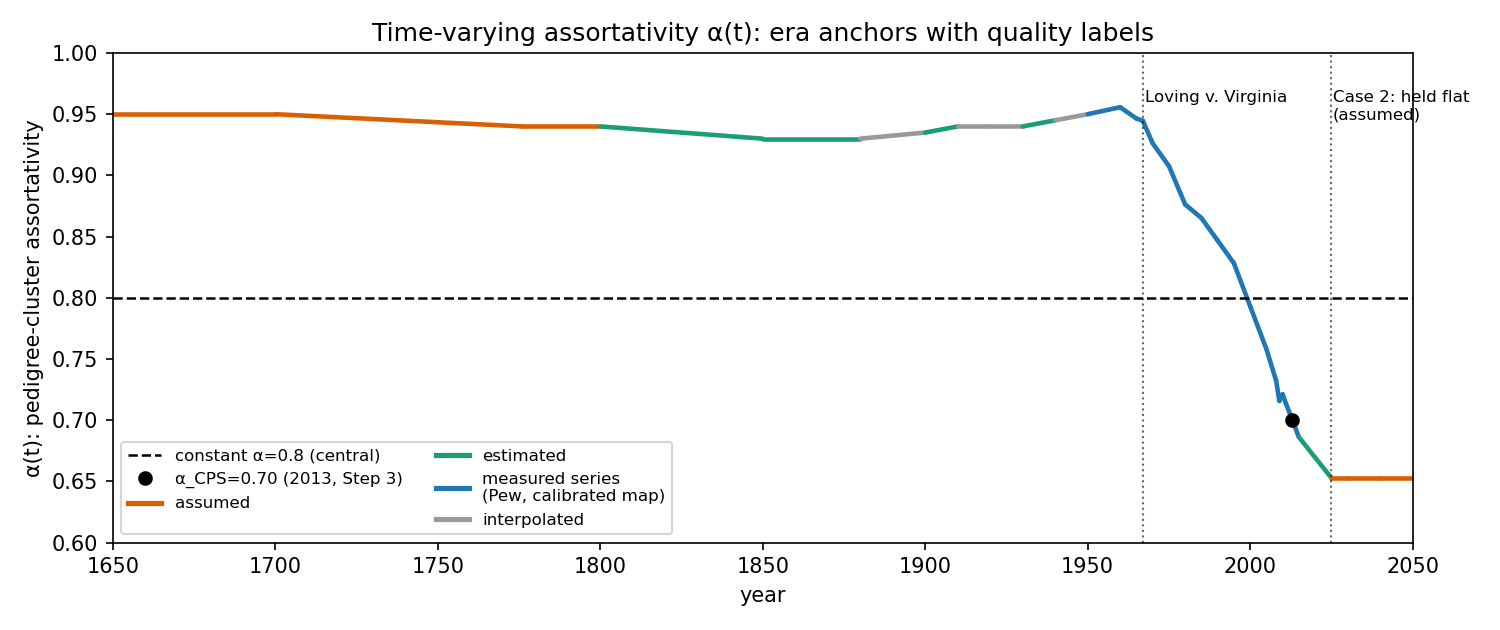
\includegraphics[width=\textwidth]{figs/alpha_schedule.png}
\caption{The $\alpha(t)$ schedule 1650--2050 with quality-colored
segments, constant-0.8 reference, $\alpha_{\mathrm{CPS}}=0.66$ (2013)
marker, and the Case-2 hold.}
\label{fig:alpha-t-sched}
\end{figure}

\begin{figure}[htbp]
\centering
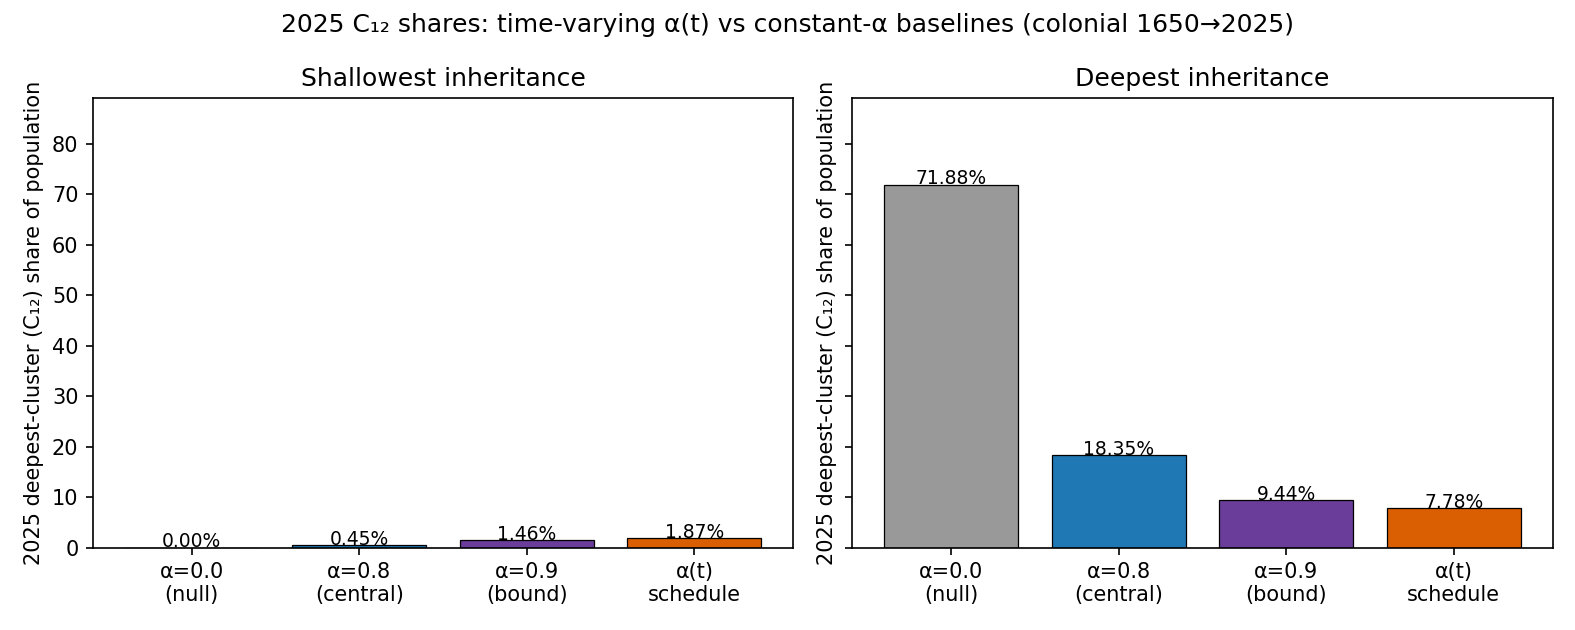
\includegraphics[width=\textwidth]{figs/alpha_t_comparison.png}
\caption{2025 $C_{14}$ shares --- constant-$\alpha$ bracket (0.0 null,
\textbf{0.8} central, 0.9 bound) vs the $\alpha(t)$ schedule, $n=14$.
Shallowest: the schedule exceeds the 0.9 bound (path dependence).
Deepest: the schedule undershoots constant-0.8 (recent mixing dominates).}
\label{fig:alpha-t-comp}
\end{figure}

\paragraph{Maternal bottleneck.}  The $\min(W^{\mathrm{pat}},
W^{\mathrm{mat}})$ marriage function makes the \emph{maternal}
population the limiting sex under male-skewed immigration, sharply
reducing births vs the old $\sigma=0.5$ assumption: decomposition at
shallowest $\alpha=0.8$ gives 2025 totals 300.2\,M (old $\sigma$, old
$\mu$), 241.5\,M (new $\sigma$, old $\mu$), 324.9\,M (old $\sigma$,
new $\mu$), and \textbf{259.0\,M} (new $\sigma$, new $\mu$) --- all
four model families now land at $\approx 259$\,M in 2025.  The anchor
fit is worse than the old run: worst error \textbf{$-29.3\%$ at 1830}
(old: $-13.4\%$).  The emigration rate $\varepsilon$ is deliberately
\emph{not} recalibrated to close the gap --- the mismatch is reported
honestly rather than tuned away.  The hindcast, which starts from the
measured 1980 state, is barely affected ($-2.87$\,M, $-0.8\%$ in
2024).

\subsection{Sex-specific rates: the immigrant male-share series}
The old $\sigma=0.5$ assumption is replaced by the data-driven
$\sigma(t)$ series of Fig.~\ref{fig:sigma-t} (construction in
Sec.~2.1): 0.65 \emph{assumed} (1650--1819, indentured-labor skew),
0.629 \emph{estimated} (1820--1917, HSUS period aggregate applied
annually), quota-era convergence to 0.50 by 1950 \emph{estimated},
2015--2023 measured DHS LPR-by-sex~\cite{dhs-lpr-sex} blended with an
\emph{estimated} unauthorized-stock-as-inflow proxy~\cite{dhs-unauth-table4},
2024 0.470 \emph{interpolated}, held through 2050 \emph{assumed}.  Sex
mortality differential $\mu_{\mathrm{pat}}/\mu_{\mathrm{mat}}$
(2024 $\approx 1.069$) is \emph{measured}~\cite{hld}; the level is
scaled to the aggregate CDR (\emph{estimated}).  All model families now
converge on a 2025 total of $\approx$259\,M (two-sex 258.95, religious
258.95, regional 258.95, age 259.7\,M).  The largest remaining
sex-structure uncertainty is the paternal age schedule (still the
female ASFR shape, \emph{assumed}): shifting it $\sim$2\,yr older moves
2025 $C_n$ by 2--5\,pp at $\alpha\ge0.8$ (Sec.~6.4), because the
$\min(W^{\mathrm{pat}},W^{\mathrm{mat}})$ kernel makes the older-shifted
paternal side the binding sex more often.

\begin{figure}[htbp]
\centering
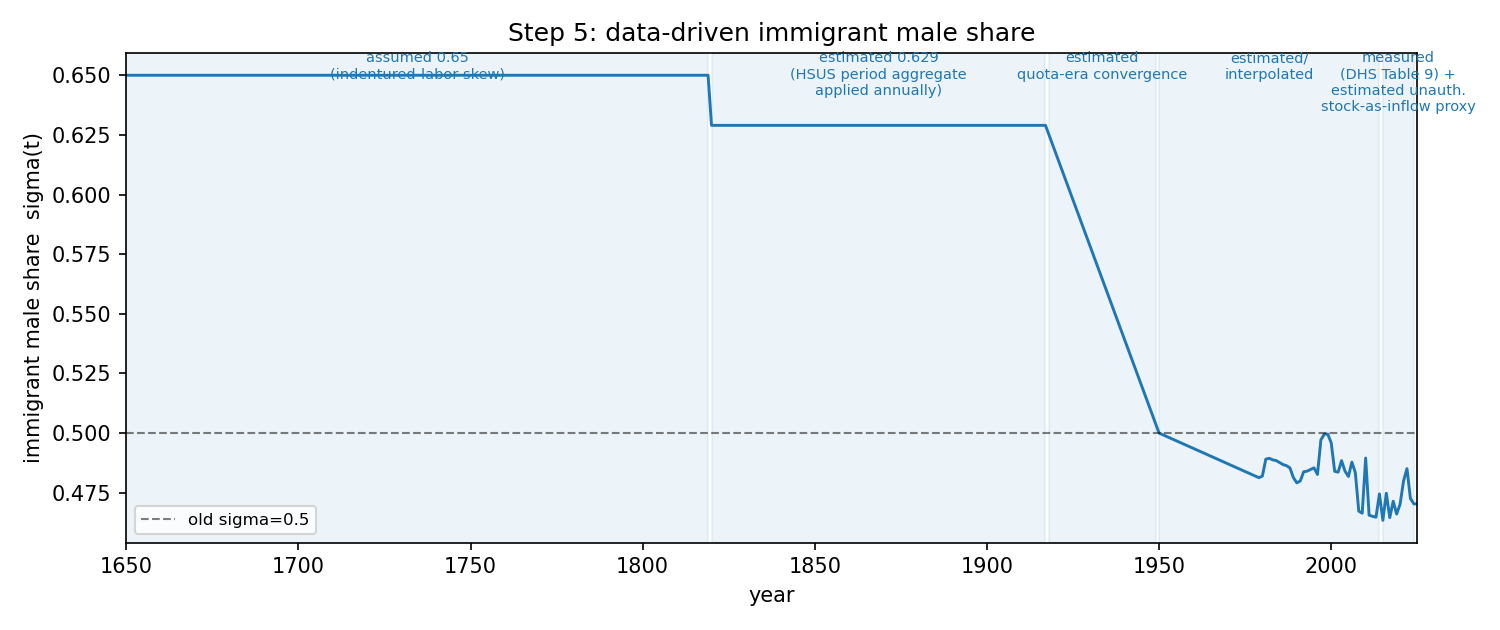
\includegraphics[width=0.65\textwidth]{figs/step5_sigma_series.png}
\caption{The immigrant male-share series $\sigma(t)$ used by all
families (labels in Sec.~2.1).  Two era breaks are visible: 1820 (the
HSUS 0.629 aggregate takes over from the assumed 0.65) and 1950 (parity
reached), then the DHS measured + proxy era from 2015 (0.470 in 2024).}
\label{fig:sigma-t}
\end{figure}

\subsection{Case 1: colonial run, 1650--2025}
The historical run (Figs.~\ref{fig:ts-shallowest}, \ref{fig:ts-deepest})
gives the 2025 ordering at $n=14$: shallowest $C_{14}$ is 0.00\%,
\textbf{0.45\%}, 1.46\% for $\alpha=0.0,0.8,0.9$; deepest 71.88\%,
\textbf{18.35\%}, 9.44\%.  The two-sex and religious $n=14$ models agree
to 0.004\,pp at central $\alpha$ (shallowest), making the four model
families apples-to-apples.  The paternal share of the 2025 population
is 50.09\% in every run.

\begin{figure}[htbp]
\centering
\begin{minipage}{0.49\textwidth}\centering
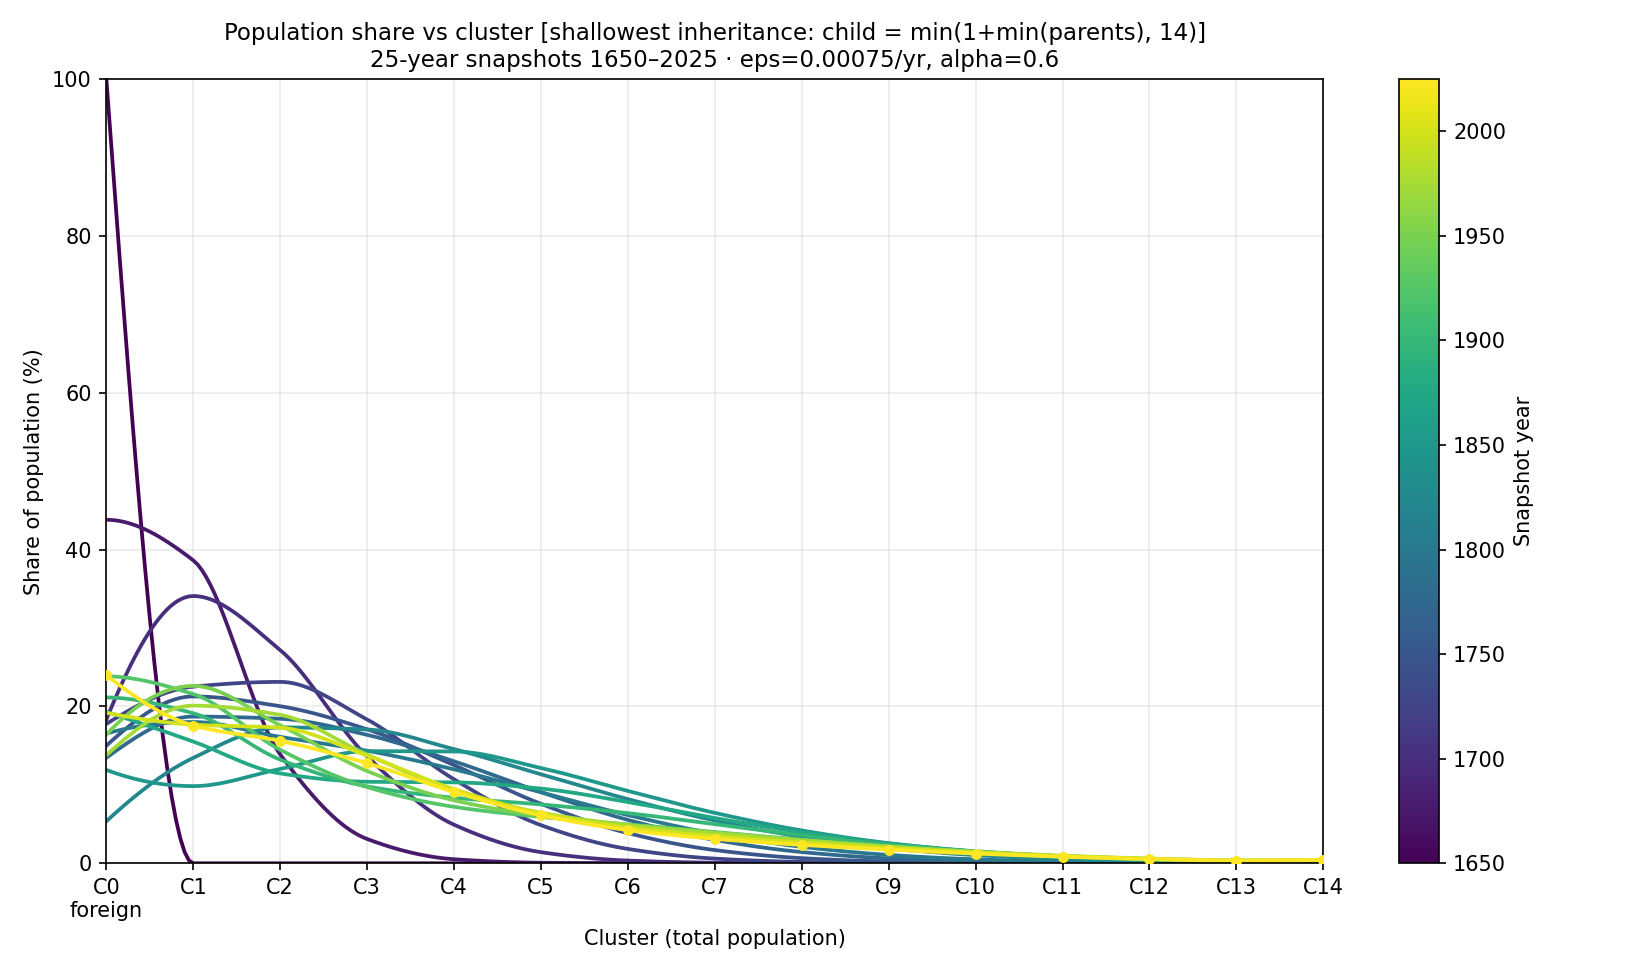
\includegraphics[width=\textwidth]{figs/dist_shallowest_inheritance_linear.png}
\caption{\textbf{(a) Shallowest:} $C_{14}$ reaches \textbf{0.45\%} by 2025
($\alpha=0.8$); deep clusters replenish only through
deep$\times$deep intermarriage.}
\label{fig:ts-shallowest}
\end{minipage}\hfill
\begin{minipage}{0.49\textwidth}\centering
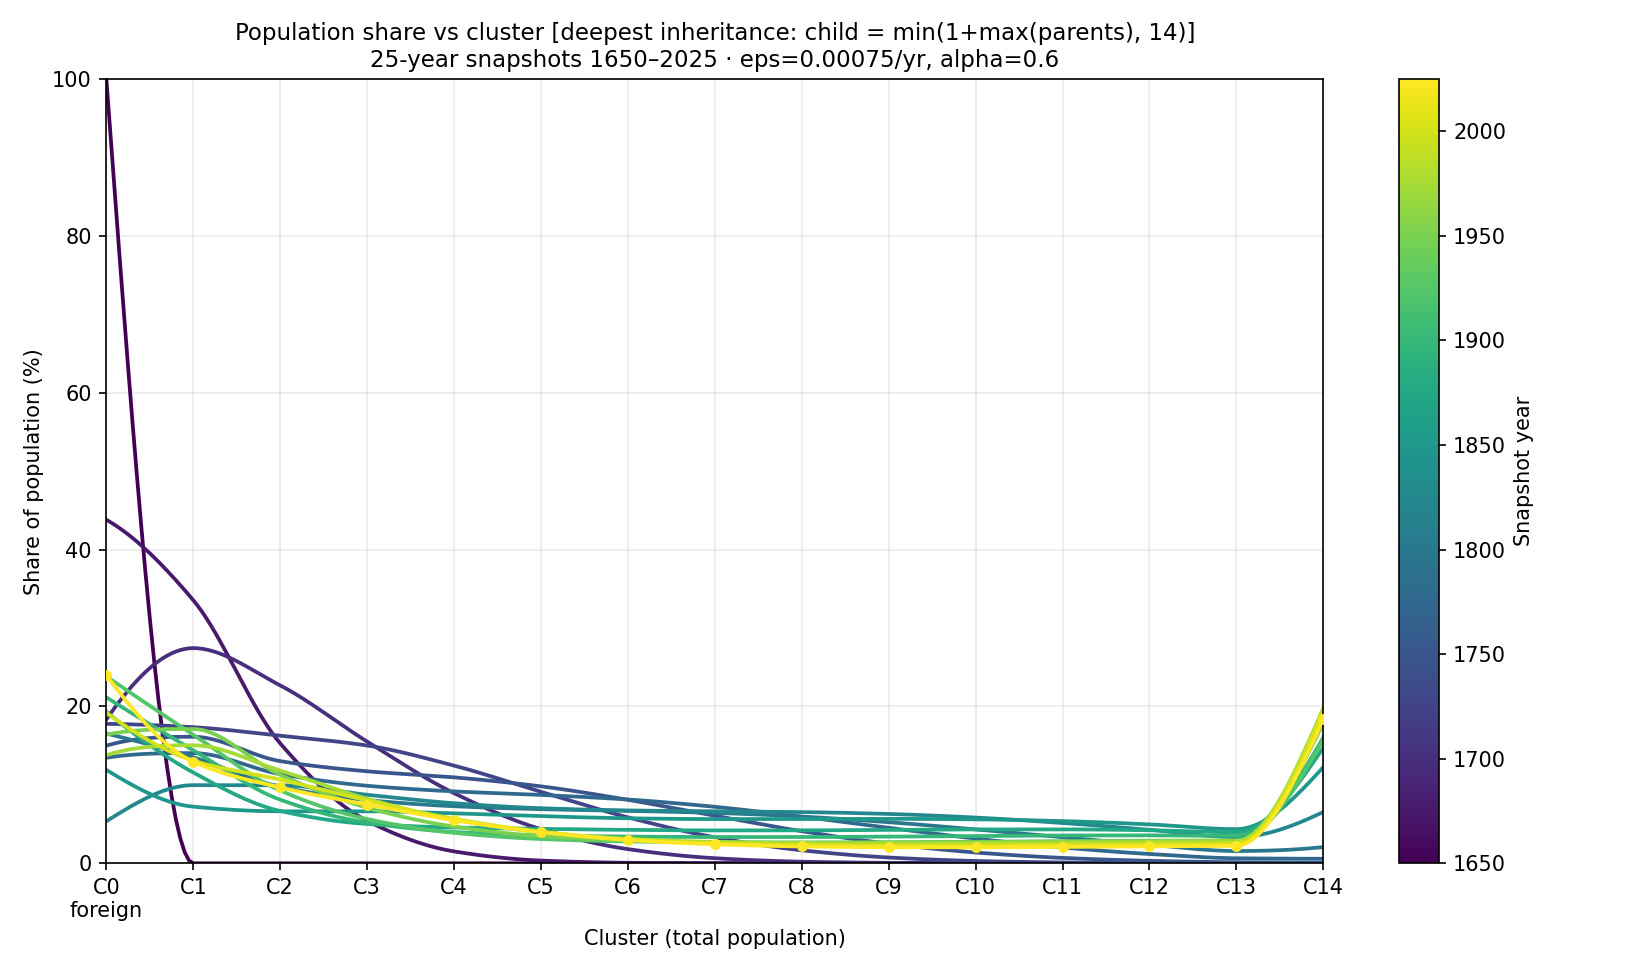
\includegraphics[width=\textwidth]{figs/dist_deepest_inheritance_linear.png}
\caption{\textbf{(b) Deepest:} $C_{14}$ reaches \textbf{18.35\%} by 2025;
with no downward pull, lineages ratchet upward and accumulate at the cap.}
\label{fig:ts-deepest}
\end{minipage}
\end{figure}

\subsection{Case 2: 2025--2050 projection}
From the exact Case-1 2025 handoff state: the 2050 deepest-cluster bar
chart by rule and $\alpha$ (Fig.~\ref{fig:proj-cn}) and the 2050
totals/deepest shares table above.  The religious Case-2 projection is
reported with the religious results (Sec.~\ref{sec:religious}).

\begin{figure}[htbp]
\centering
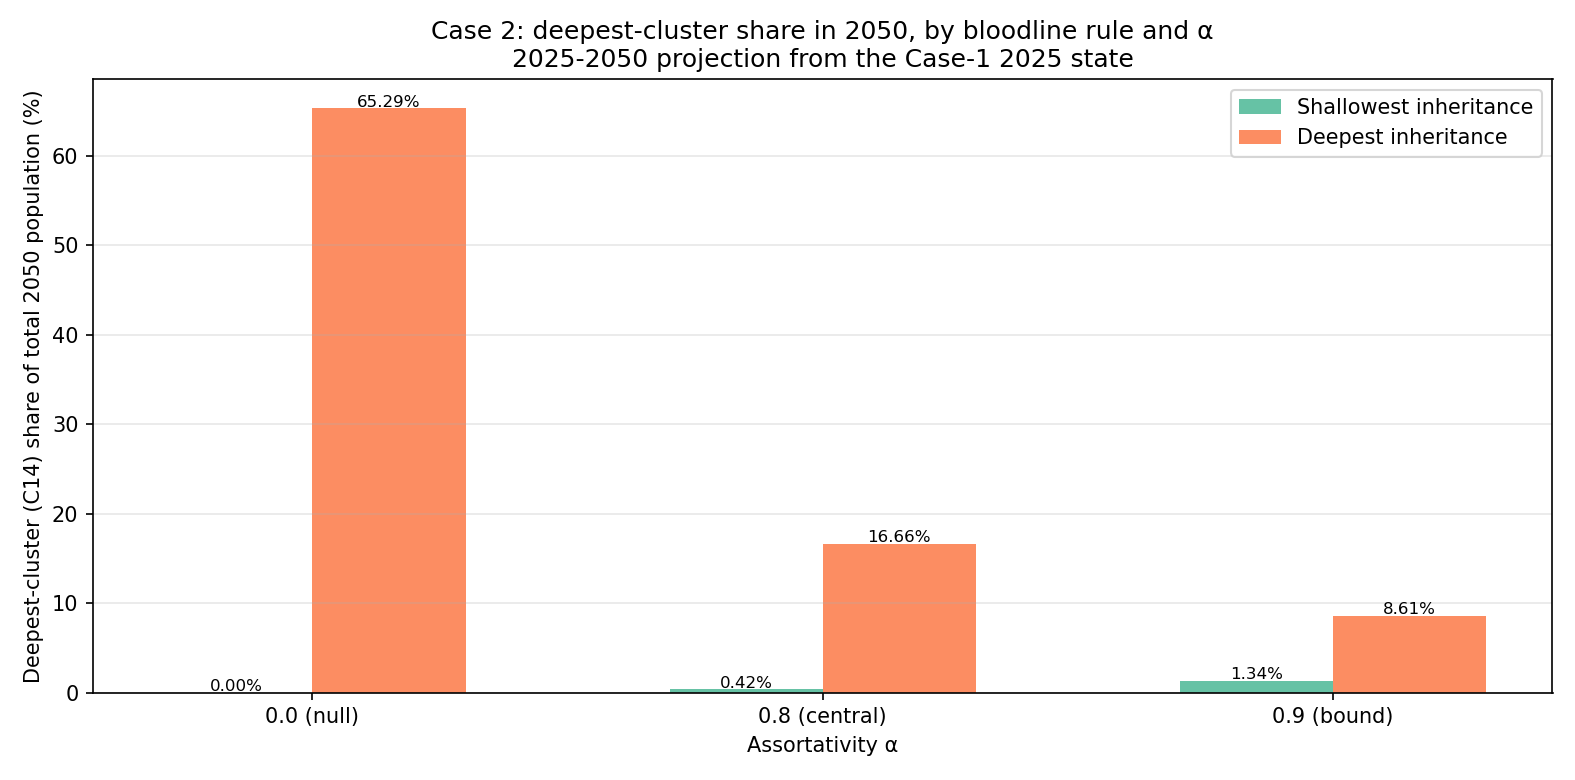
\includegraphics[width=0.55\textwidth]{figs/proj2050_cn_by_rule.png}
\caption{Deepest-cluster ($C_{14}$) share of the 2050 population vs
assortativity $\alpha$, by bloodline rule (Case-2 projection
2025--2050 from the Case-1 2025 state).  Bracket: 0.0 (null),
\textbf{0.8} (central), 0.9 (bound).}
\label{fig:proj-cn}
\end{figure}

\subsection{Deeper cluster resolution: $n=14$ and the resolved tail}
The cluster depth is now $n=14$ in \emph{all} model families --- the
religious runs no longer differ from the rest (Sec.~6.8's old
$n=12$ vs $n=14$ incomparability is gone).  $375/14=26.8$\,yr per
generation matches the measured mean generation interval
\emph{independently}: the truncation choice is self-consistent, not
just convenient.  Four runs of the two-sex Case-1 model at
$\alpha=0.8$ (Fig.~\ref{fig:tail-shape}):

\begin{center}
\small
\begin{tabular}{@{}lrrrr@{}}
\toprule
Rule & $n{=}12$ & \textbf{$n{=}14$} & $n{=}18$ & $n{=}24$ \\
\midrule
Shallowest $C_n$ & 1.33\% & \textbf{0.45\%} & 0.03\% & 0.00\% \\
Deepest $C_n$ & 22.74\% & \textbf{18.35\%} & 9.33\% & 1.31\% \\
\bottomrule
\end{tabular}
\end{center}
Totals stay bit-identical across $n$ (mass is only relabeled), and the
cap is \emph{bit-conserved}: $C_{14}$ at $n=14$ equals
$\sum_{d\ge14}$ at $n=18$ and $n=24$ under \emph{both} rules (0.4488\% /
18.3527\%) --- no mass piles up at the truncation.  Under shallowest
inheritance the tail decays geometrically: beyond $C_{18}$ only
0.034\% remains.  Under deepest inheritance the cap \emph{intentionally}
accumulates the ratchet mass --- this is the rule's physics, not a
numerical artifact --- and resolving it to $n=24$ shows the deep tail is
nearly flat ($\sim$2.2\% per cluster from $C_{12}$ to $C_{17}$, declining
to 0.68\% at $C_{23}$); the invariant is $\sum_{d\ge14}$, which is
conserved exactly.  \textbf{Verdict}: $n=14$ is a faithful,
bit-conserved truncation under both rules; the cap does not distort the
dynamics, and the continuous-index alternative is unnecessary.

\begin{figure}[htbp]
\centering
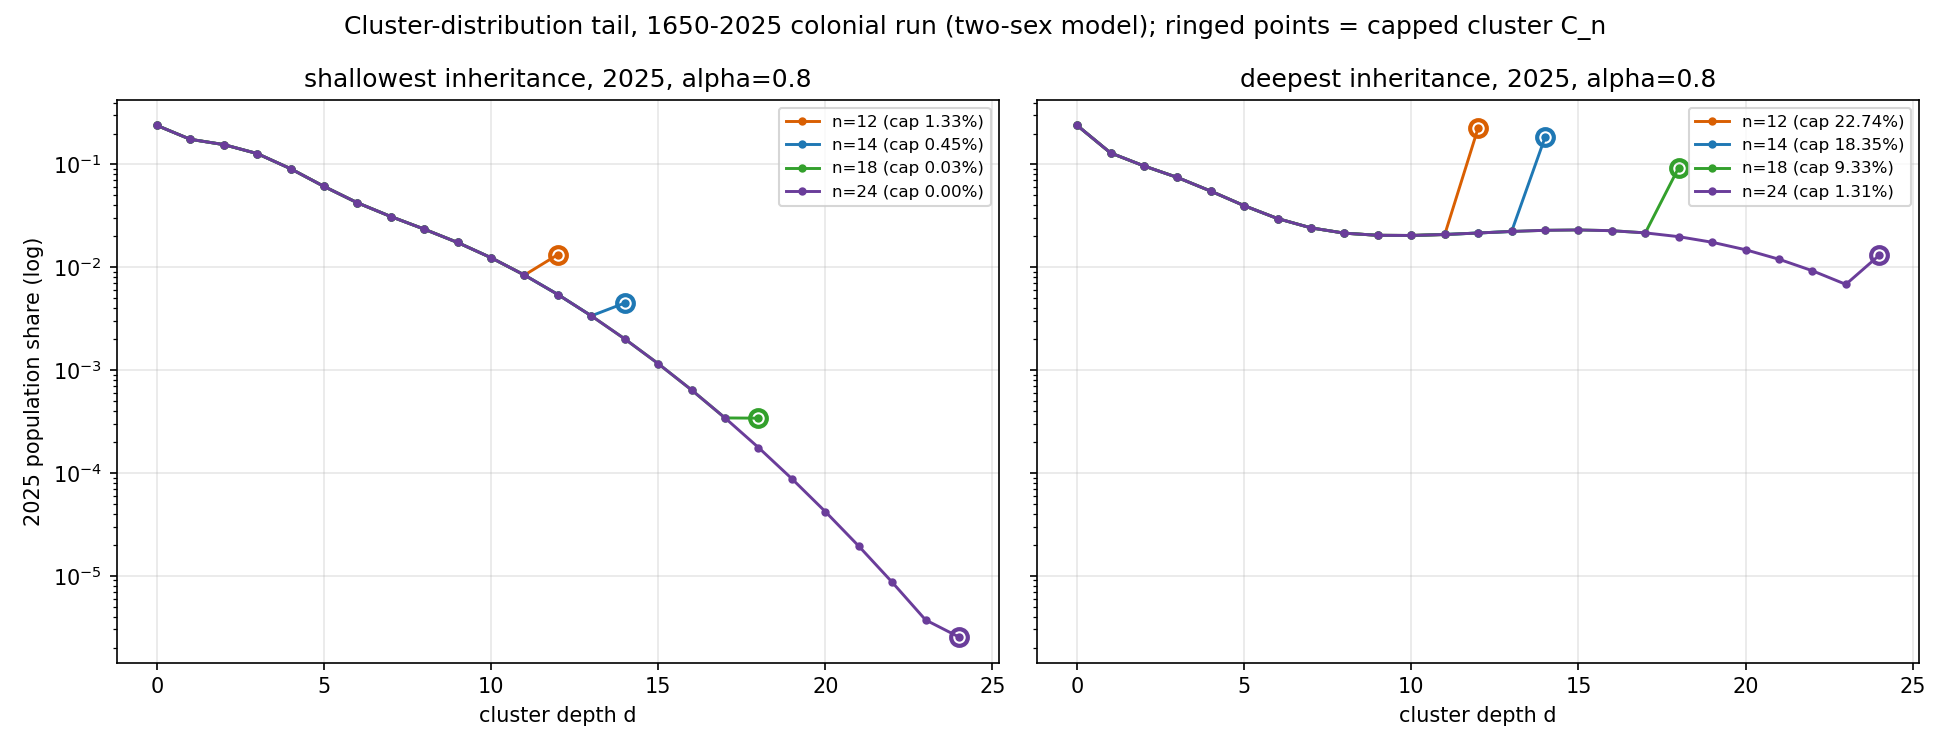
\includegraphics[width=0.68\textwidth]{figs/step6_tail_shape.png}
\caption{Tail of the 2025 cluster distribution at $\alpha=0.8$,
$n=12/14/18/24$ (ringed = capped cluster).  The cap is bit-conserved:
$C_{14}$ at $n=14$ equals $\sum_{d\ge14}$ at $n=18$ and $n=24$ ---
no pile-up.  At $n=24$ the tail beyond $C_{18}$ is exhausted.}
\label{fig:tail-shape}

\vspace{0.5em}
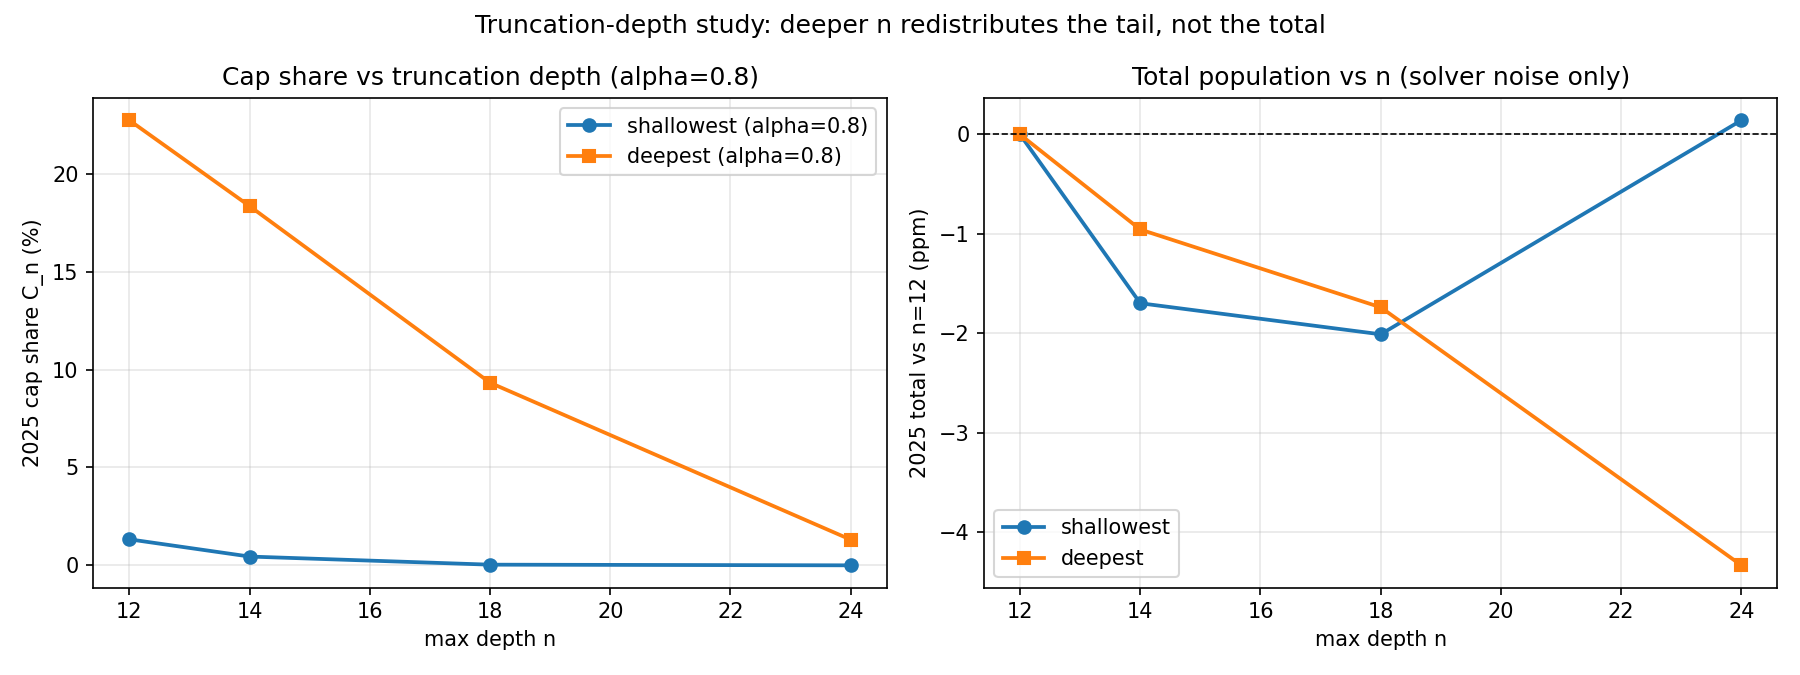
\includegraphics[width=0.45\textwidth]{figs/step6_n_comparison.png}
\caption{2025 $C_n$ share at $\alpha=0.8$ for $n=12,14,18,24$, both
rules.  $n=14$ is the operating point; $n=12$ inflated the deep share
$\sim$3$\times$ by truncating the tail.}
\label{fig:tail-cmp}
\end{figure}

\subsection{Age structure: resolved tail amplifies deep concentration}
The 540-state colonial run at $\alpha=0.8$ (Sec.~\ref{sec:age}; $n=14$):
2025 $C_{14}$ is \textbf{1.62\%} (age) vs 0.45\% (aggregate) under the
shallowest rule and \textbf{38.90\%} vs 18.35\% under the deepest rule
(Fig.~\ref{fig:age-dist}) --- age structure concentrates deep mass in
old cohorts, and the deepest rule ratchets that reservoir to the cap.
The wavefront experiment
(Fig.~\ref{fig:wavefront}; closed population, constant rates) remains
valid as a \emph{rate} measurement, independent of $n$: the age front
advances $\sim$one rung per human generation (floor at the minimum
parental age, 15\,yr); under high colonial fertility the aggregate
climbs $\approx$1.9$\times$ faster (no floor), while under low modern
fertility it is mass-accumulation-limited and runs slower.  2025 totals:
age-structured 259.7\,M vs aggregate 258.95\,M vs $\sim$342\,M actual;
anchor validation worst error $-24.0\%$ in 2024.

\paragraph{Male-fertility sensitivity (age-structured model).}  The
default equal-schedule proxy (female ASFR shape for fathers,
\emph{assumed}) vs a paternal schedule shifted $\sim$2\,yr older:
shallowest $\alpha=0.8$ 2025 $C_{14}$ 1.62\%$\to$0.79\% ($-0.83$\,pp, $-51$\%
rel.), deepest 38.90\%$\to$28.66\% ($-10.23$\,pp, $-26$\% rel.); totals
$-4.9$\% everywhere (older-shifted paternal weights make the paternal
side the binding sex in the $\min$ kernel more often).  A material
modeling uncertainty ($\approx$1--10\,pp on 2025 $C_{14}$ at
$\alpha\ge0.8$): the proxy is retained as default but stays labeled
\emph{assumed}.

\begin{figure}[htbp]
\centering
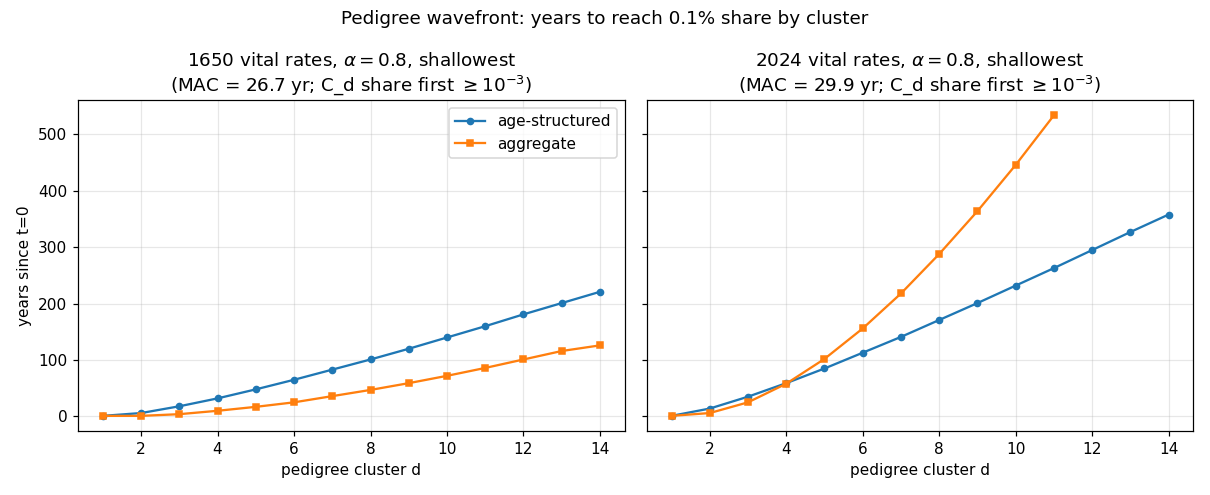
\includegraphics[width=0.55\textwidth]{figs/wavefront_comparison.png}
\caption{Pedigree wavefront: years for each cluster to reach 0.1\%
share (closed population, constant rates, shallowest rule, $\alpha=0.8$).
Left (1650 rates): the aggregate front climbs $\approx$1.9$\times$ faster ---
the missing generation-delay artifact (no 15\,yr parental-age floor).
Right (2024 rates): the aggregate is mass-accumulation-limited and runs
slower.}
\label{fig:wavefront}

\vspace{0.5em}
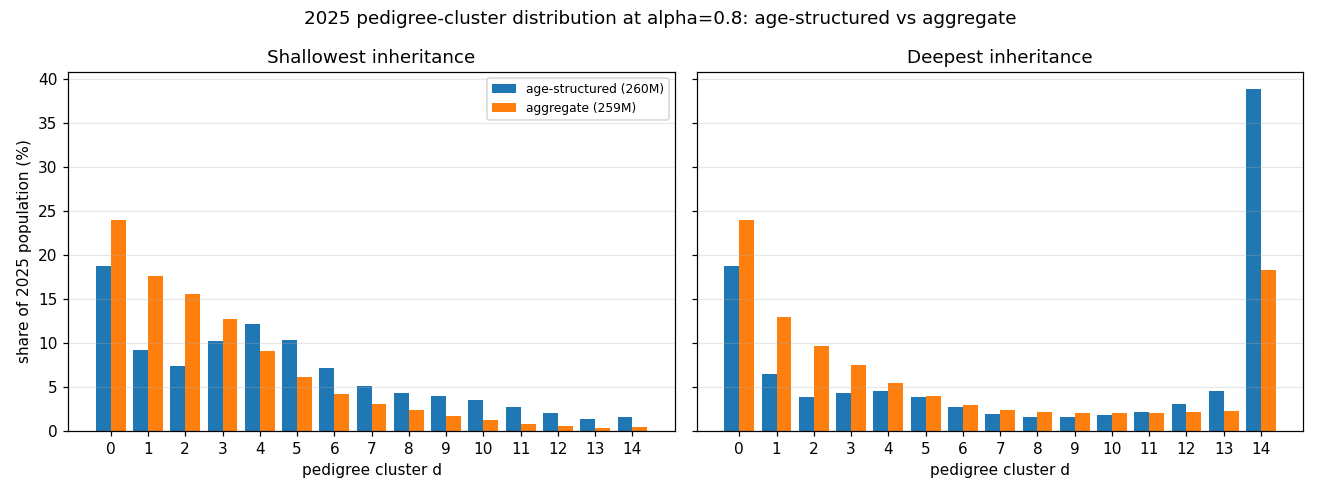
\includegraphics[width=0.55\textwidth]{figs/cluster_dist_2025.png}
\caption{2025 cluster distributions at $\alpha=0.8$, $n=14$:
age-structured vs aggregate, shallowest (left) and deepest (right).
$C_{14}$: 1.62\% vs 0.45\% (shallowest), 38.90\% vs 18.35\% (deepest) ---
age structure amplifies deep concentration, especially under the deepest rule.}
\label{fig:age-dist}
\end{figure}

\subsection{Regional compartments: the Midwest runs deepest}
Case-1 2025 $C_{14}$ by region at $\alpha=0.8$ (Sec.~\ref{sec:regional};
national 0.47\% / 1.40\%):

\begin{center}
\small
\begin{tabular}{@{}lcccc@{}}
\toprule
Rule & NE & MW & South & West \\
\midrule
Shallowest & 0.36\% & 0.53\% & 0.49\% & 0.43\% \\
Deepest & 1.14\% & 1.54\% & 1.47\% & 1.31\% \\
\bottomrule
\end{tabular}
\end{center}
The ordering MW $>$ South $>$ West $>$ NE holds at all three $\alpha$
and both rules (Figs.~\ref{fig:reg-dist}, \ref{fig:reg-traj}): the
Midwest receives the smallest immigration share (11.3\%) so its deep
lineages are least diluted, the Northeast (24.0\%) most diluted; all
regions were seeded from the NE/South founder pool via the measured
migration network.  Regions track together until $\sim$1800, then
diverge; all peak $\sim$1980 and decline under immigration dilution.
Region totals are emergent, not calibrated (2025: NE 39.3, MW 45.5,
South 115.9, West 58.2\,M) --- regional vital-rate differences and
calibration are future work.  Case-2 2050: ordering unchanged (shallowest
NE 0.34 / MW 0.49 / S 0.45 / W 0.40\%, national 0.43\%; deepest 13.37 /
18.93 / 17.67 / 15.62\%, national 16.76\%).

\begin{figure}[htbp]
\centering
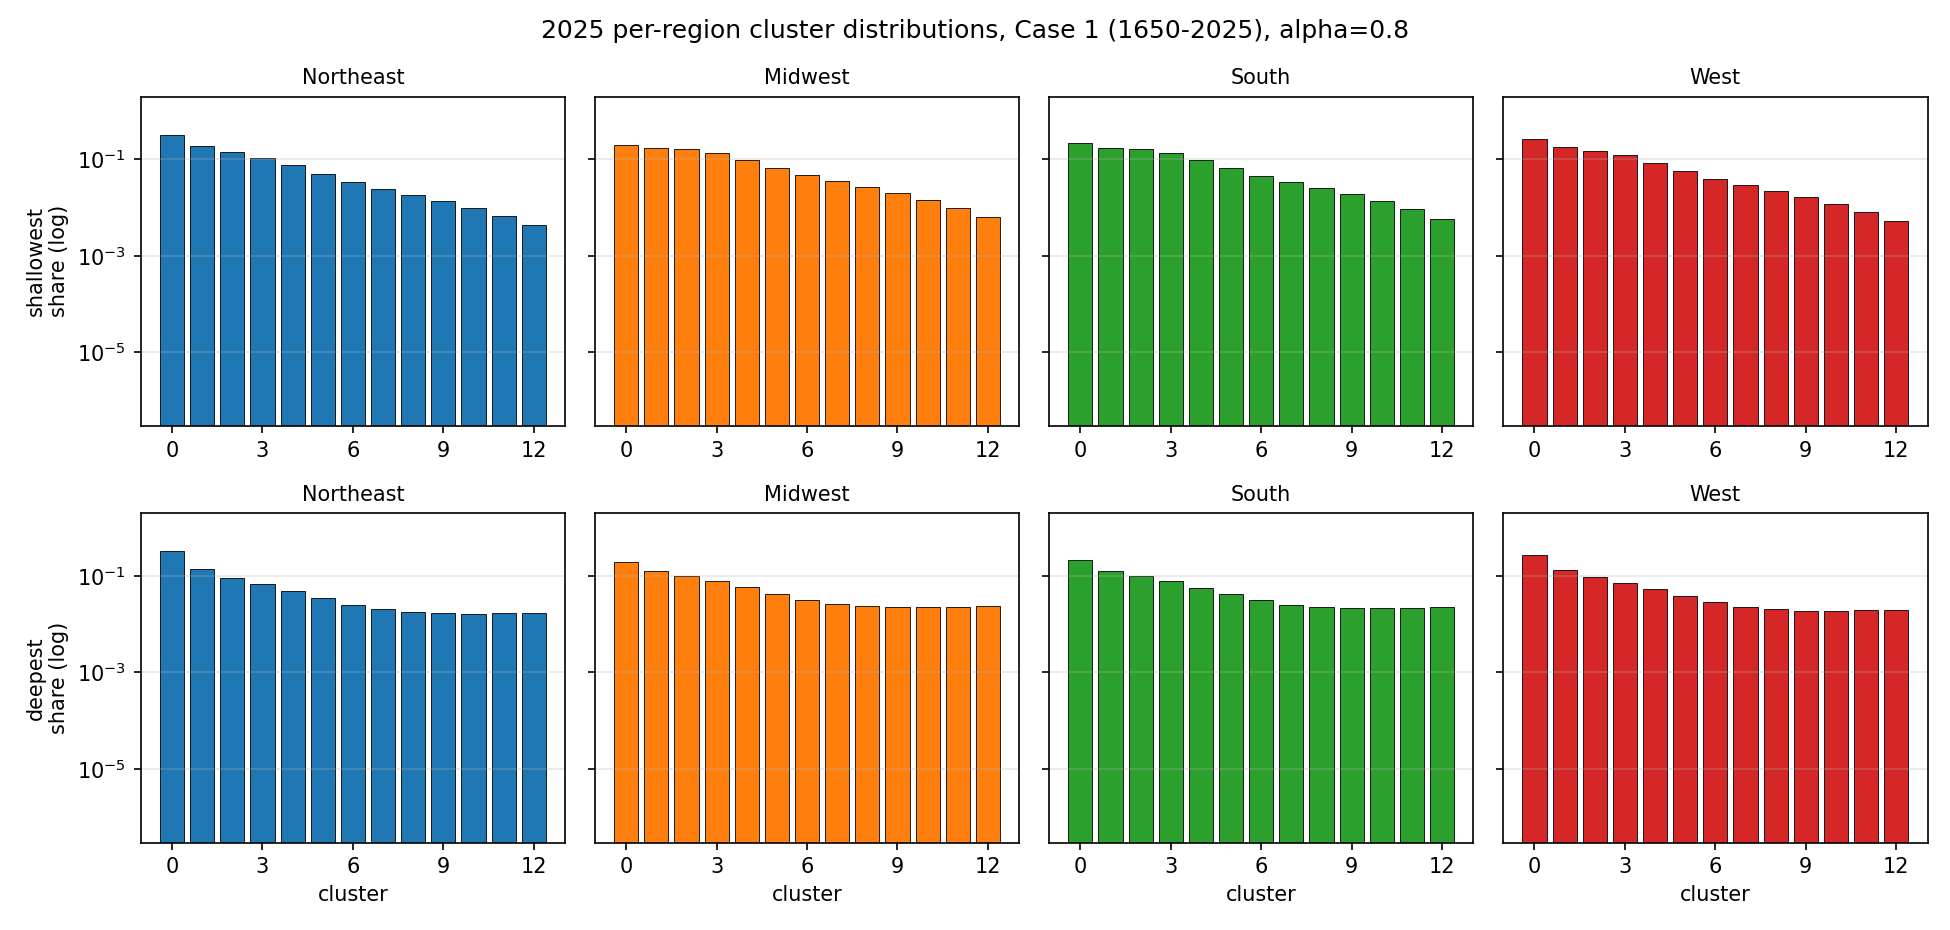
\includegraphics[width=0.5\textwidth]{figs/regional_dist_2025.png}
\caption{2025 per-region cluster distributions (Case 1, $\alpha=0.8$),
log scale: shallowest (top), deepest (bottom).  Midwest (11.3\% immigration)
deepest; Northeast (24.0\%) shallowest.}
\label{fig:reg-dist}

\vspace{0.5em}
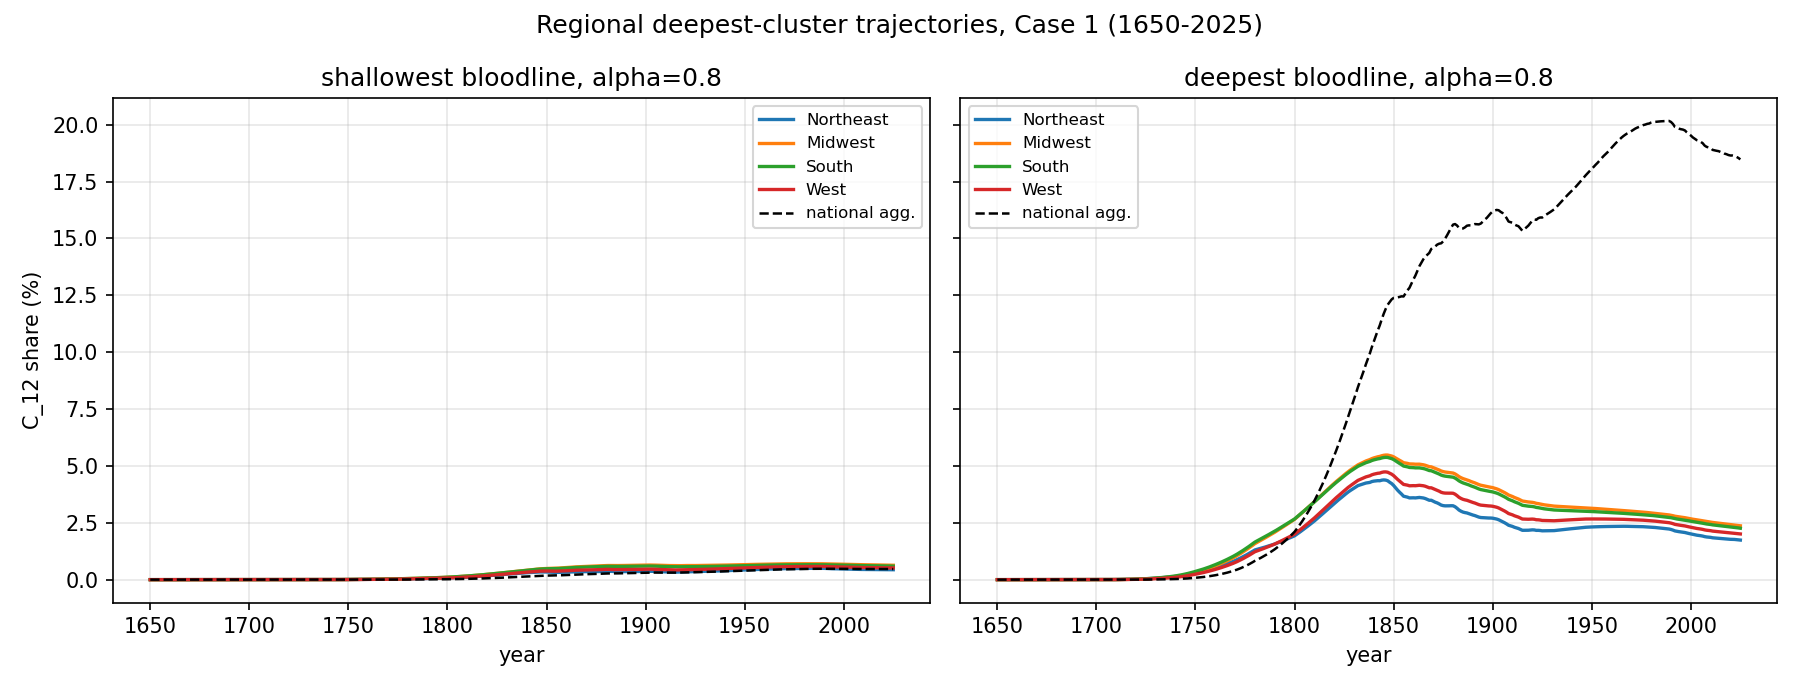
\includegraphics[width=0.5\textwidth]{figs/regional_deepest_traj.png}
\caption{Regional $C_{14}$ trajectories 1650--2025 ($\alpha=0.8$),
both rules plus national.  Regions diverge after $\sim$1800, peak
$\sim$1980, decline under immigration dilution.}
\label{fig:reg-traj}
\end{figure}

\subsection{CPS parental-nativity calibration of $\alpha$}
\label{sec:cps}
CPS ASEC 2024 Table~1 gives the annual second-generation share
2005--2024, 10.5\%$\to$12.6\% (\emph{measured}~\cite{cps-asec-2024});
P23-214 gives the 2013 split: second generation 11.7\%, of whom 59\%
have two foreign-born parents, i.e.\ 6.90\% of the population
(\emph{measured}$\times$\emph{measured}~\cite{p23-214}).  Model
mapping: shallowest $C_1$ = US-born with $\ge$1 foreign-born parent (the CPS
second generation); deepest $C_1$ = US-born children of \emph{two}
immigrants.  The calibration statistic is the ratio
deepest-$C_1$/shallowest-$C_1$ versus the CPS 59\%: the underlying people
are identical in both runs (only the cluster \emph{labeling} differs by
rule), so the ratio is the model's exact analog of the CPS split and
cancels the colonial run's total-population level error.  Result:
$\alpha_{\mathrm{CPS}}=\mathbf{0.66}$ (model ratio 59.0\% vs CPS
59\%; Fig.~\ref{fig:cps}).  Absolute-level checks prefer
$\alpha\ge0.8$ but are level-biased: the colonial run overstates the
immigrant stock ($C_0(2013)=19.2\%$ vs CPS first generation 12.9\%).
Decision: $|0.66-0.8|=0.14$ is not material $\to$ \textbf{keep
$\alpha=0.8$ as central}, bracketed by the ratio fit (0.66) and the
absolute-series preference ($\ge 0.9$).

\begin{figure}[htbp]
\centering
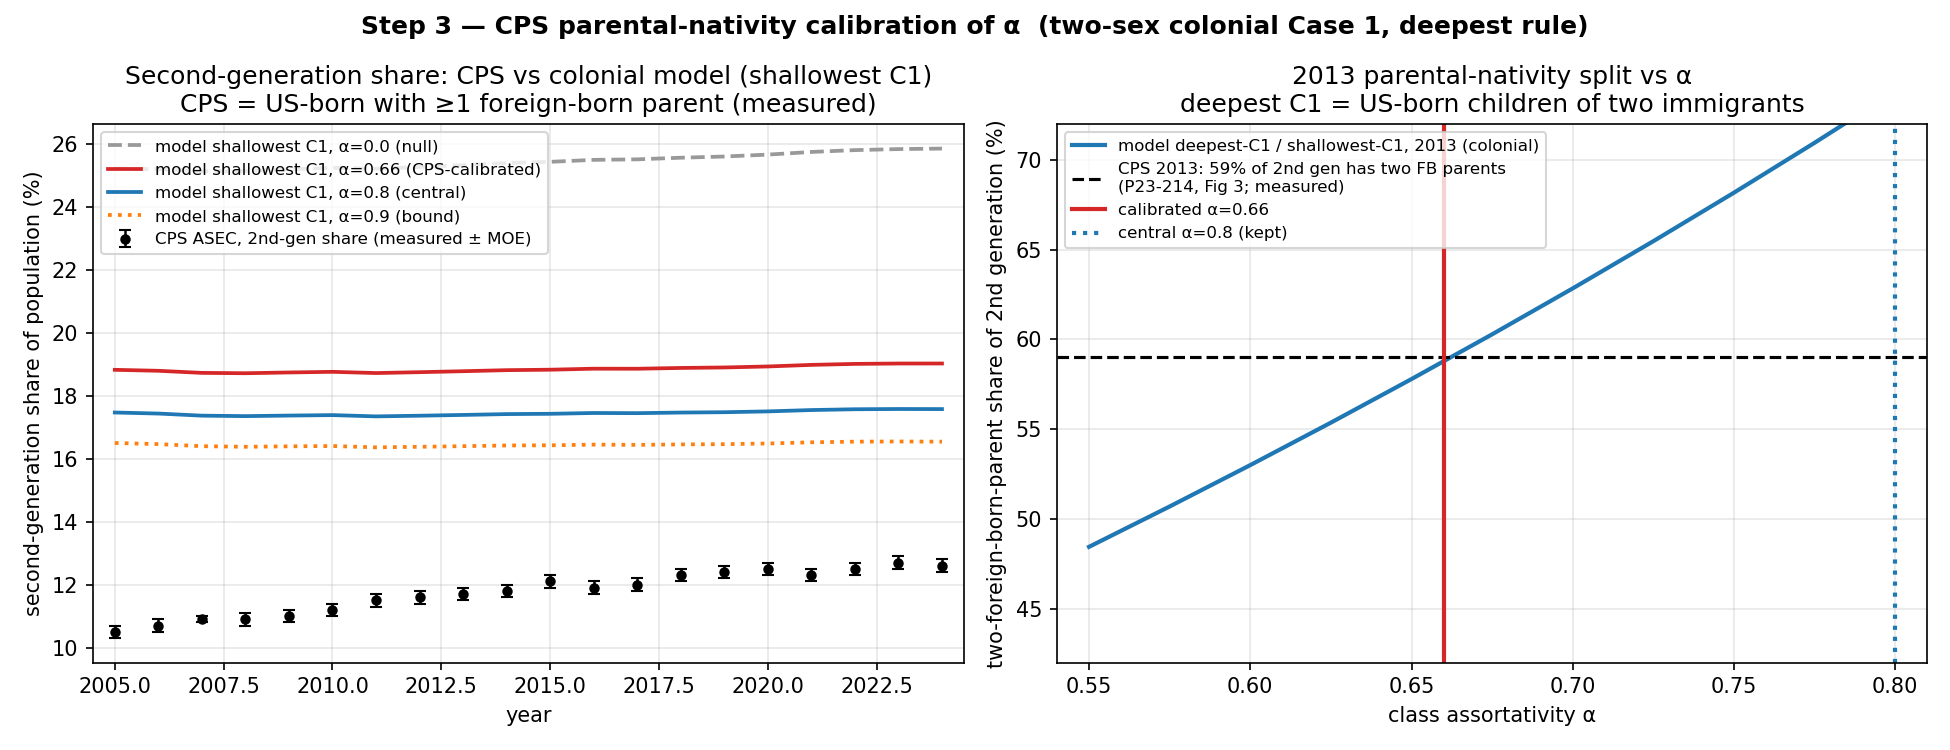
\includegraphics[width=0.55\textwidth]{figs/cps_calibration.png}
\caption{CPS calibration of $\alpha$.  Left: CPS ASEC second-generation
share 2005--2024 (measured $\pm$ MOE) vs model shallowest $C_1$.
Right: 2013 two-parent share (deepest-$C_1$/shallowest-$C_1$) vs $\alpha$;
CPS 59\% anchor (P23-214): calibrated $\alpha=0.66$, central
$\alpha=0.8$ kept.}
\label{fig:cps}
\end{figure}

\subsection{Religious dimension: composition and deepest clusters at $n=14$}
\label{sec:religious}
The religious extension (Sec.~2.2) was run 1650--2025 at $n=14$ ($240$
ODEs) for both bloodline rules (shallowest and deepest) and
$\alpha=0.0,0.8,0.9$, with the
group endogamies $\rho_g$ of Table~1, the era immigrant compositions
$\iota_g(t)$, and disaffiliation ramping 1970--1990 to the calibrated
$\delta_{\max}=8\times10^{-3}\,\mathrm{yr}^{-1}$.  Totals are 258.95\,M in
2025 in every run (religion is compositional: disaffiliation is internal),
and the exact balance $dN/dt=I+B-(\mu+\varepsilon)N$ holds to
$\sim 10^{-15}$ with disaffiliation active.

\paragraph{2025 religious composition vs.\ Pew.}  Modeled 2025 shares
(deepest rule, $\alpha=0.8$; identical across both rules and $\alpha$ to the
printed precision, since group totals do not depend on the child-cluster
rule) against the Pew 2023--24 Religious Landscape Study adult
shares~\cite{pew-rls-2025}:

\begin{center}
\small
\begin{tabular}{@{}lcccccccc@{}}
\toprule
 & pro & cat & mor & jew & mus & dhr & oth & una \\
\midrule
Model 2025 & 43.3\% & 17.9\% & 0.2\% & 3.2\% & 2.2\% & 2.7\% & 2.6\% & 27.9\% \\
Pew 2023--24 & 40\% & 19\% & $\sim$1.6\% & 2\% & 1\% & 2\% & $\sim$1\% & 29\% \\
\bottomrule
\end{tabular}
\end{center}
The unaffiliated share is the calibrated quantity (27.9\% vs.\ 29\% Pew);
the rest is a sanity check, not a fit.  Mormon is under-shot (0.2\% vs.\
$\sim$1.6\%): the model has no conversion \emph{into} Mormonism and no
fertility differential, while disaffiliation drains the group at the full
$\delta(t)$ --- a named limitation.  Figure~\ref{fig:rel-shares} shows
the full 1650--2025 trajectories with the Pew anchors.

\paragraph{Deepest-cluster shares at $n=14$.}  The 2025 $C_{14}$ share of the
total population, by rule and $\alpha$:

\begin{center}
\small
\begin{tabular}{@{}lccc@{}}
\toprule
Rule & $\alpha{=}0.0$ (null) & \textbf{0.8} (central) & $0.9$ (bound) \\
\midrule
Shallowest inheritance & 0.00\% & \textbf{0.45\%} & 1.47\% \\
Deepest inheritance & 68.80\% & \textbf{17.93\%} & 9.34\% \\
\bottomrule
\end{tabular}
\end{center}
The ordering and the $\alpha$-direction match the two-sex $n=14$ runs
(Sec.~6.1); the two families agree to within 0.5\,pp everywhere, so the
religious extension is a genuine apples-to-apples refinement.

\paragraph{Deepest clusters by religious group.}  Within-group $C_{14}$
shares in 2025 ($\alpha=0.8$; Fig.~\ref{fig:rel-cn-group}) run from
24.51\% (Protestant) and 18.65\% (unaffiliated) down to $\approx 1.6$\%
for post-1965-immigrant groups (Muslim, Hindu/Buddhist) under deepest
inheritance; under shallowest, all groups sit below 0.7\%.

\paragraph{Case-2 religious projection, 2025--2050.}  From the Case-1
2025 state ($n=14$): 2050 total 279.7\,M; unaffiliated 27.9\%$\to$\textbf{36.4\%}
(rule-independent, the one-way disaffiliation flow continued at the
calibrated $8\times10^{-3}$/yr --- a flagged artifact, not a forecast;
two-way switching is future work, Sec.~7).  2050 $C_{14}$ at
$\alpha=0.8$: shallowest \textbf{0.42\%}, deepest \textbf{16.25\%}.

\begin{figure}[htbp]
\centering
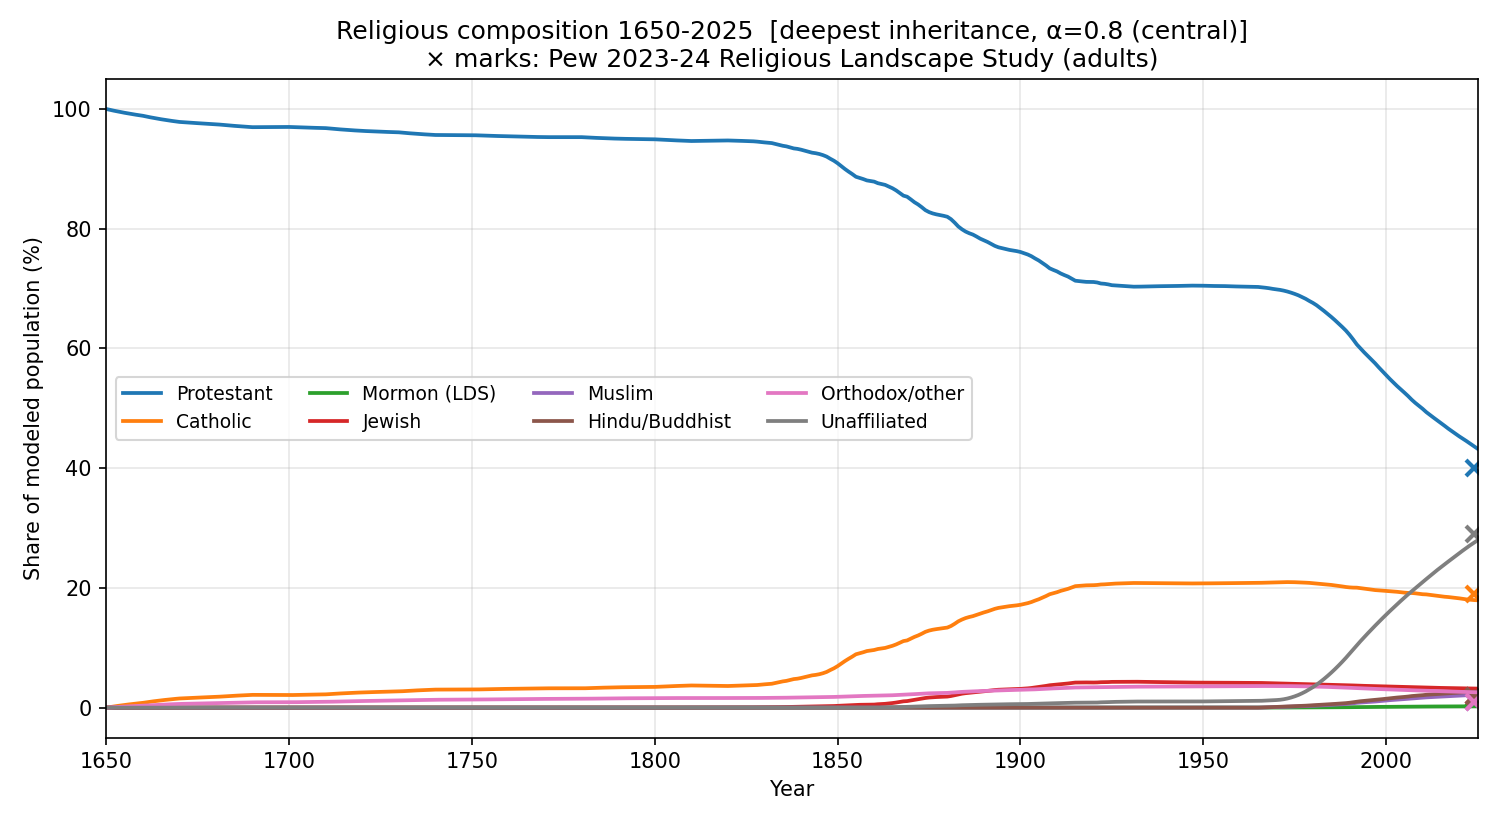
\includegraphics[width=0.5\textwidth]{figs/fig_religious_shares.png}
\caption{Religious composition 1650--2025 (deepest, $\alpha=0.8$,
$n=14$).  $\times$: Pew 2023--24 adult shares~\cite{pew-rls-2025}.
Unaffiliated (gray) is the calibrated quantity: disaffiliation ramps
1970--1990 to $\delta_{\max}=8\times10^{-3}$/yr, landing at 27.9\%
vs.\ Pew's 29\%.}
\label{fig:rel-shares}

\vspace{0.5em}
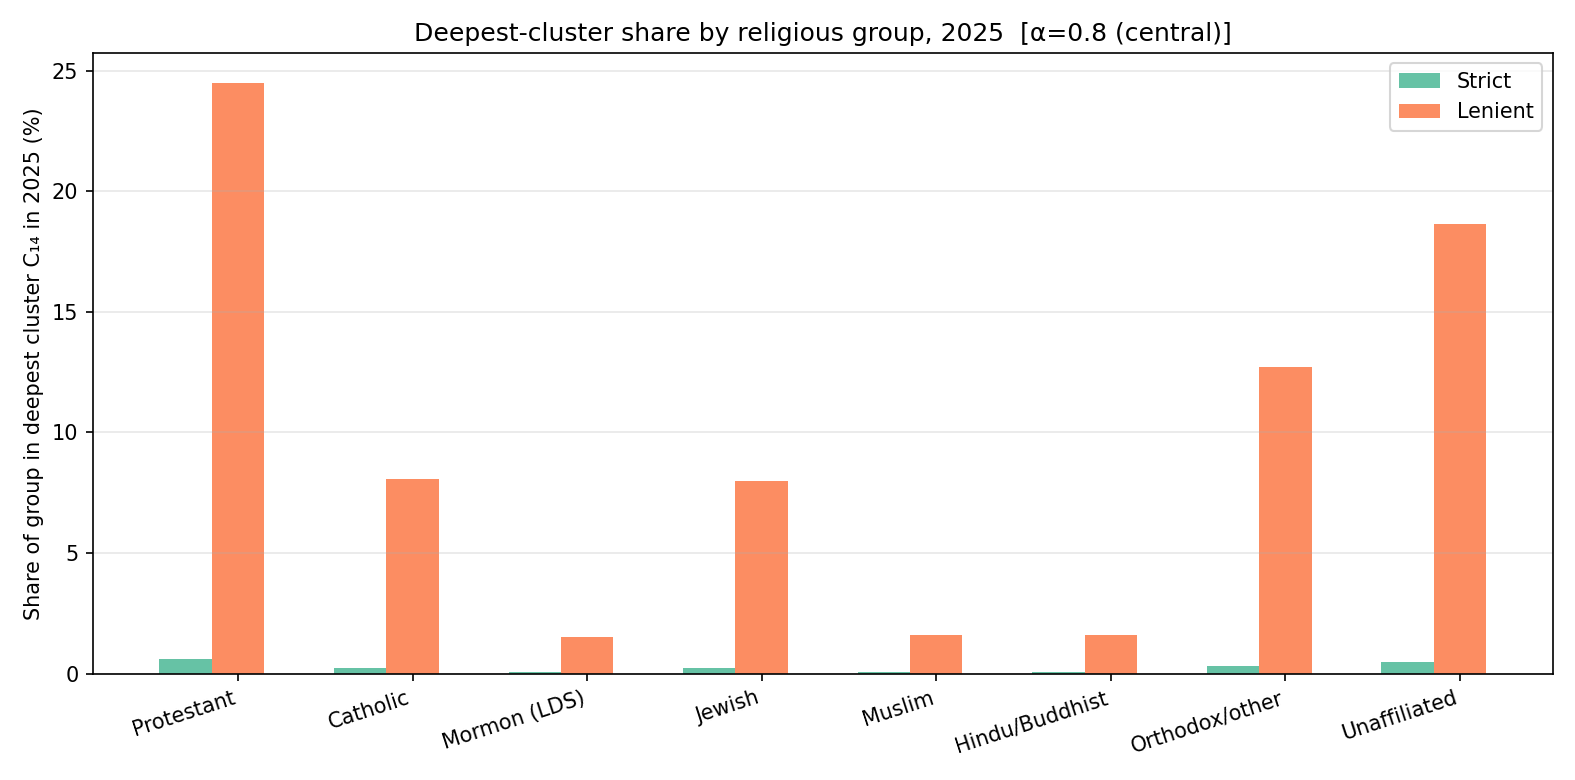
\includegraphics[width=0.5\textwidth]{figs/fig_religious_cn_by_group.png}
\caption{Deepest-cluster ($C_{14}$) share \emph{within} each religious
group in 2025, by rule ($\alpha=0.8$, $n=14$).  Long-tenure groups run
deep (Protestant 1.70\%, unaffiliated 1.35\%); post-1965-immigrant
groups stay shallow ($\approx 0.17\%$).}
\label{fig:rel-cn-group}
\end{figure}

\begin{figure}[htbp]
\centering
\begin{minipage}[t]{0.46\textwidth}\centering
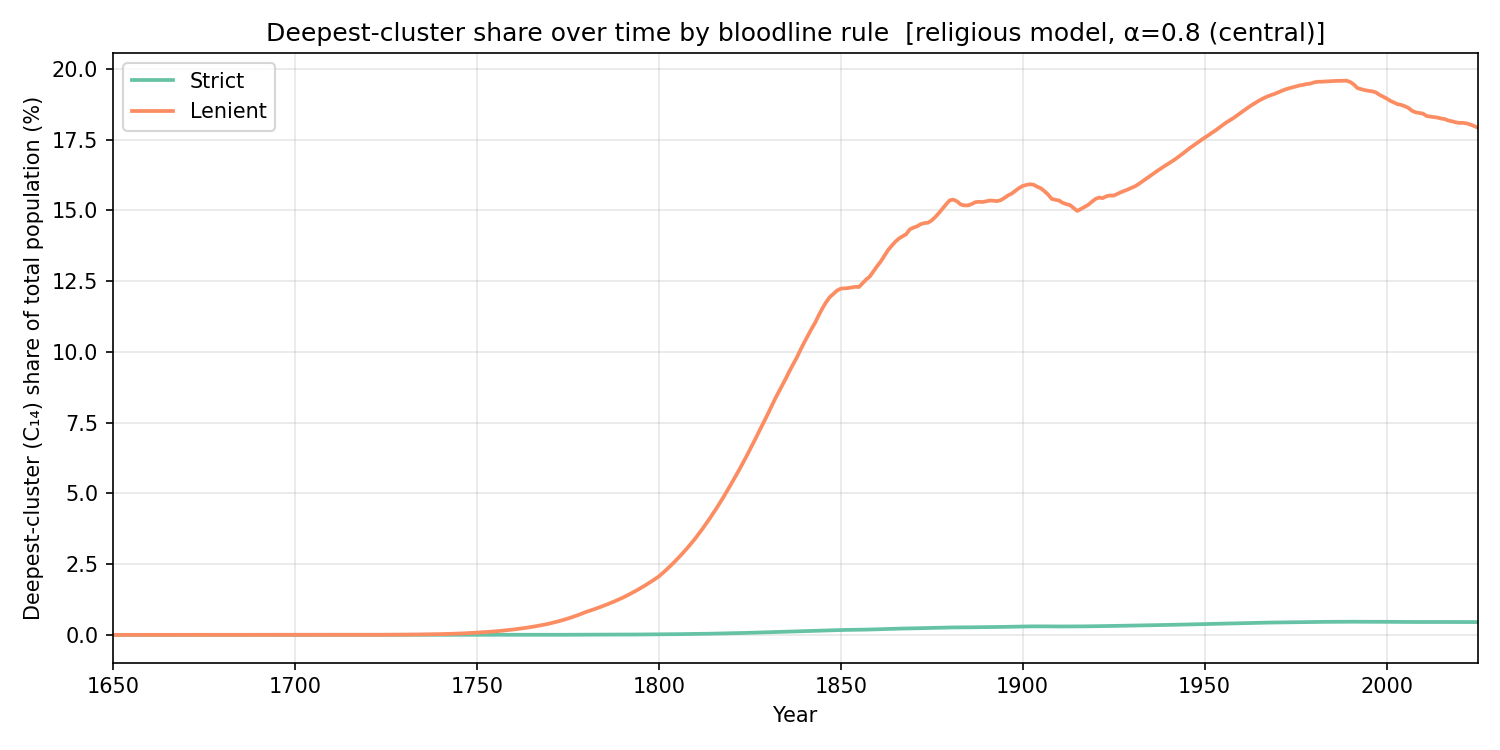
\includegraphics[width=\textwidth]{figs/fig_cn_total_series.png}
\caption{Deepest-cluster ($C_{14}$) share of the total population over
time, by rule (religious model, $\alpha=0.8$, $n=14$).}
\label{fig:rel-cn-series}
\end{minipage}\hfill
\begin{minipage}[t]{0.46\textwidth}\centering
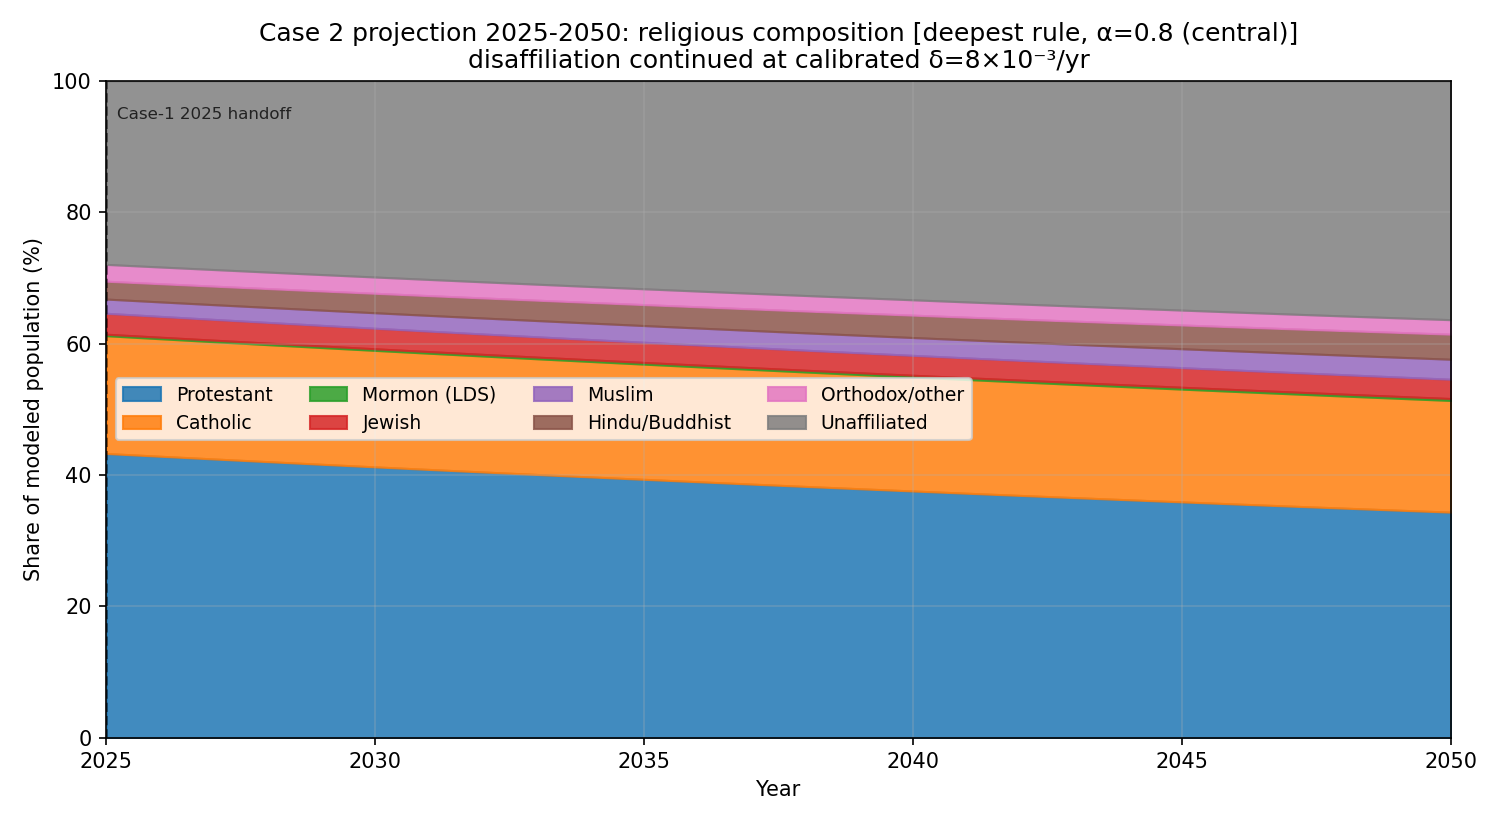
\includegraphics[width=\textwidth]{figs/proj2050_religious_shares.png}
\caption{Case-2 religious composition 2025--2050 (deepest,
$\alpha=0.8$, $n=14$).  Unaffiliated 27.9\%$\to$36.4\%; Protestant
43.3$\to$34.3\%; Muslim 2.2$\to$3.0\%; Hindu/Buddhist 2.7$\to$3.8\%.}
\label{fig:proj-rel-shares}
\end{minipage}
\end{figure}

\subsection{Stochastic colonial era: the deterministic trajectory is unbiased}
\label{sec:stochastic}
$\tau$-leaping ensembles ($N=300$ trajectories, 1650--1800, all-$C_0$
initial condition) under both inheritance rules, testing the ODE for
finite-population bias, deep-cluster coefficients of variation, and
discrete establishment years.
Is the ODE a fair description while the colonial population is small
(50,368 in 1650)?  This section writes down the jump process, the
$\tau$-leaping algorithm, and the simulation procedure in full.
Is the ODE a fair description while the colonial population is small
(50,368 in 1650)?  This section writes down the jump process, the
$\tau$-leaping algorithm, and the simulation procedure in full.

\paragraph{The jump process.}  The state is the integer population vector
$\mathbf{X}(t)\in\mathbb{N}^{2(n+1)}$ (people; block order
$[\mathrm{pat},\mathrm{mat}]$; 30 states at $n=14$).  Three reaction
classes fire, with propensities (people/yr) and stoichiometry:
\begin{align}
  \emptyset &\xrightarrow{\,a_{\mathrm{imm},\alpha}\,}
    (0,\alpha), &
    a_{\mathrm{imm},\alpha}(\mathbf X) &= \sigma_\alpha(t)\,I(t),
    \quad \sigma_{\mathrm{pat}}=\sigma(t),\
    \sigma_{\mathrm{mat}}=1-\sigma(t), \label{eq:stoch-imm} \\
  (q,\mathrm{pat}) + (r,\mathrm{mat})
    &\xrightarrow{\,a_{qr,\alpha'}\,}
    (q,\mathrm{pat}) + (r,\mathrm{mat}) + (g(q,r),\alpha'), &
    a_{qr,\alpha'}(\mathbf X) &=
      \begin{cases} s\,J_{qr}(\mathbf X), & \alpha'=\mathrm{pat} \\
      (1-s)\,J_{qr}(\mathbf X), & \alpha'=\mathrm{mat}
      \end{cases} \label{eq:stoch-birth} \\
  (d,\alpha) &\xrightarrow{\,a_{d,\alpha}\,}
    \emptyset, &
    a_{d,\alpha}(\mathbf X) &=
      (\mu_\alpha(t)+\varepsilon)\,X_{d,\alpha}. \label{eq:stoch-death}
\end{align}
Parents are catalytic: they appear on both sides of the birth reaction
and are not consumed.  The mating flux $J_{qr}$ is exactly the ODE
kernel of Sec.~\ref{sec:rags},
\begin{equation}
  J_{qr}(\mathbf c) = B(\mathbf c)\,
    \big[\alpha\,\delta_{qr}\,m^{\mathrm{pat}}_q
    + (1-\alpha)\,m^{\mathrm{pat}}_q m^{\mathrm{mat}}_r\big],
    \qquad
    B = \min(W^{\mathrm{pat}},W^{\mathrm{mat}}),\quad
    W^{\mathrm{pat}} = \sum_d \beta_{d,\mathrm{pat}}\,c_{d,\mathrm{pat}},
    \quad
    m^{\mathrm{pat}}_q =
    \frac{\beta_{q,\mathrm{pat}}\,c_{q,\mathrm{pat}}}{W^{\mathrm{pat}}},
  \label{eq:stoch-flux}
\end{equation}
evaluated here on the integer counts $\mathbf X$; the child-sex split
$s:(1{-}s)$ in \eqref{eq:stoch-birth} is the exact Poisson thinning of
the $J_{qr}$ event stream.
\paragraph{Mean-field limit.}  The family is density-dependent in the
sense of Kurtz~\cite{kurtz-1970}: immigration \eqref{eq:stoch-imm} and
death \eqref{eq:stoch-death} are linear in $\mathbf X$, and the mating
flux \eqref{eq:stoch-flux} is homogeneous of degree~1 in $\mathbf X$
(the weights $m$ are scale-free), so the scaled process
$\bar{\mathbf X}^{(\lambda)}=\mathbf X^{(\lambda)}/\lambda$ converges
to the Case-1 ODE trajectory $\mathbf c(t)$ as $\lambda\to\infty$.
A $\lambda=1000$ population-scaled check ($N=30$ trajectories, shallowest,
$\alpha=0.8$) reproduces the ODE with total max
$|\mathrm{rel.\ dev.}|=7.7\times10^{-5}$, confirming the Kurtz limit
in the code.

\paragraph{$\tau$-leaping algorithm.}  Propensities are frozen over each
leap (explicit Euler on the jump process~\cite{gillespie-1976,gillespie-2001}).
Given state $\mathbf X$ at $t$ and step $\tau$:
\begin{enumerate}
  \item \textbf{Births:} for every mating-pair type $(q,r)$,
    \begin{equation}
      K_{qr,\mathrm{pat}} \sim \mathrm{Poisson}(s\,J_{qr}(\mathbf X)\,\tau),
      \qquad
      K_{qr,\mathrm{mat}} \sim \mathrm{Poisson}((1-s)\,J_{qr}(\mathbf X)\,\tau),
      \label{eq:stoch-leap-birth}
    \end{equation}
    the child-sex split by exact Poisson thinning.
  \item \textbf{Deaths/emigration:} exact per-leap for the constant
    per-capita rate over the leap,
    \begin{equation}
      L_{d,\alpha} \sim \mathrm{Binomial}\!\big(X_{d,\alpha},\
        1-e^{-(\mu_\alpha(t)+\varepsilon)\tau}\big),
      \label{eq:stoch-leap-death}
    \end{equation}
    bounded by $X_{d,\alpha}$, so no state can go negative.
  \item \textbf{Immigration:}
    \begin{equation}
      I_\alpha \sim \mathrm{Poisson}(\sigma_\alpha(t)\,I(t)\,\tau).
      \label{eq:stoch-leap-imm}
    \end{equation}
  \item \textbf{State update} (birth inflow accumulated by child
    cluster $g=g(q,r)$):
    \begin{equation}
      \mathbf X(t+\tau) = \mathbf X(t)
        + \sum_{q,r}\sum_{\alpha'\in\{\mathrm{pat},\mathrm{mat}\}}
          K_{qr,\alpha'}\,\mathbf e_{(g(q,r),\alpha')}
        + I_{\mathrm{pat}}\,\mathbf e_{(0,\mathrm{pat})}
        + I_{\mathrm{mat}}\,\mathbf e_{(0,\mathrm{mat})}
        - \sum_{d,\alpha} L_{d,\alpha}\,\mathbf e_{(d,\alpha)},
      \label{eq:stoch-leap-update}
    \end{equation}
    with $\mathbf e_{(d,\alpha)}$ the unit vector of state $(d,\alpha)$.
\end{enumerate}
The step is adaptive,
\begin{equation}
  \tau = \min\big(0.5,\ \mathrm{LEAP\_EPS}/r_{\max}(t)\big)\ \mathrm{yr},
  \qquad r_{\max}(t) = \max(\beta,\mu)+\varepsilon,
  \label{eq:stoch-tau}
\end{equation}
in the Cao--Gillespie--Petzold style~\cite{cao-gillespie-petzold-2006}:
because $J$ is homogeneous degree-1 with scale-free shares, bounding the
relative state change ($\mathrm{LEAP\_EPS}=0.002$) bounds the relative
propensity change.  Convergence tests show the $\tau$ error
\emph{compounds} through the generation chain:
$\mathrm{LEAP\_EPS}=0.05$ puts the 1800 $C_{14}$ share 15\% below the
ODE, $0.01$ puts it 3.2\% low, $0.002$ puts it 0.6\% low (totals off by
$1.6\times10^{-3}$/$4\times10^{-4}$/$2\times10^{-5}$) --- so a too-large
$\tau$ would mimic a ``stochastic deficit''; at production $\tau$ the
residual bias sits below the noise floor ($\sim$7,950 leaps/trajectory).

\paragraph{Simulation procedure.}  Ensembles: shallowest/deepest
$\times$ $\alpha\in\{0.8,0.0\}$, $N=300$ trajectories, 1650--1800
($\sim$3.9\,M by 1800), from the all-$C_0$ 1650 initial condition
(50,368 people, $\sigma$-split between the sexes) --- the same founding
bottleneck as the deterministic colonial run.  Drivers and ICs are
identical to that run (inputs.csv, $\sigma(t)$, sex-specific $\mu(t)$,
$\varepsilon=7.5\times10^{-4}$/yr, $s=0.512$).  The ensemble is
vectorized over the trajectory axis (all $N$ trajectories advanced in
one leap loop), pseudo-random numbers from NumPy's
\texttt{default\_rng} with fixed seeds, yearly snapshots recorded; from
them: ensemble-mean vs ODE $z$-scores and relative deviations,
per-cluster CVs at 1800, extinction fractions (share of trajectories
with $C_d=0$), median establishment years, and the CV$<1$\% crossover.
Four findings:
\begin{itemize}
  \item \textbf{(i) No bias.}  Ensemble-mean total vs ODE at 1800:
    $z=-0.84$ (shallowest), $z=+1.40$ (deepest), max $|$relative
    deviation$|\le6.1\times10^{-4}$ over the whole 1650--1800
    trajectory (Fig.~\ref{fig:stoch-mean}).  The mean-field check
    ($\lambda=1000$, $N=30$) reproduces the ODE total to
    $7.7\times10^{-5}$.
  \item \textbf{(ii) Deep-cluster mass robust.}  CV of the 1800 cluster
    share at $\alpha=0.8$: $C_6$ 0.4--0.8\%, $C_{10}$ 0.9--2.2\%,
    $C_{14}$ 9.5\% (shallowest) / 2.7\% (deepest;
    Fig.~\ref{fig:stoch-cv}) --- the deep mass is thousands of people
    by 1800, not a noise artifact.
  \item \textbf{(iii) Establishment is discrete.}  At $\alpha=0.8$,
    0/300 trajectories have empty $C_{12}$--$C_{14}$ at 1800 (both
    rules); median establishment $C_6$ $\approx$ 1662--1668, $C_{10}$
    $\approx$ 1686--1701 (Fig.~\ref{fig:stoch-est}) --- vs the ODE's
    ``all clusters $>0$ from the first birth''.
  \item \textbf{(iv) Crossover.}  CV(total) peaks 0.72\% $\sim$1710
    (population $\approx 0.25$\,M) and \emph{never reaches 1\%}:
    total-population stochasticity is negligible throughout,
    bottleneck included (Fig.~\ref{fig:stoch-fan}).
\end{itemize}
\paragraph{Verdict.} \textbf{No headline conclusion changes.}  The
deterministic colonial trajectory is unbiased for totals and all
cluster shares down to the noise floor; the ODE misleads only for
clusters with expected occupancy $\lesssim 10$ people --- far below
any reported share.

\begin{figure}[htbp]
\centering
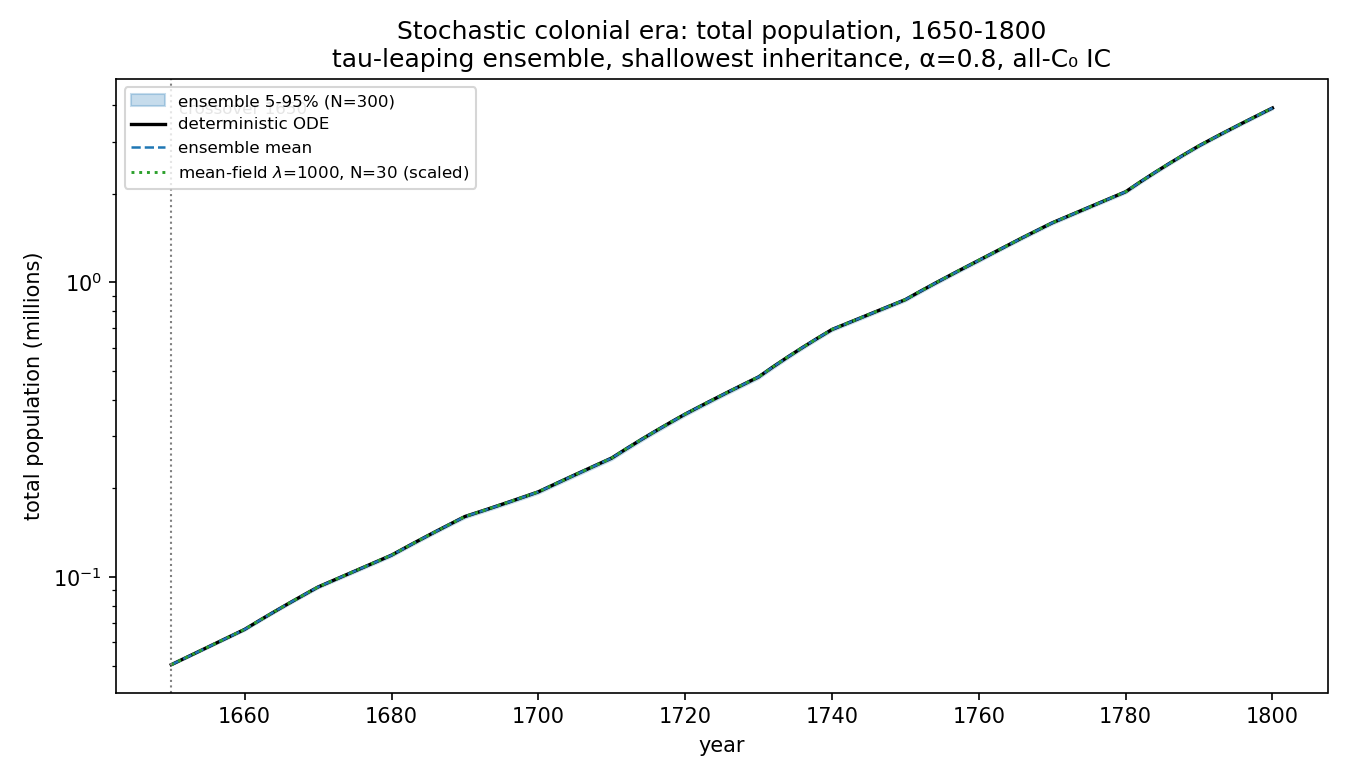
\includegraphics[width=\textwidth]{figs/stochastic_fan_total.png}
\caption{Ensemble fan 1650--1800, shallowest, $\alpha=0.8$: 5--95\% band
(razor-thin) + CV(total) vs time; the 1\% threshold is never reached
(peak 0.72\% at 1710, pop.\ $\approx 0.25$\,M).}
\label{fig:stoch-fan}
\end{figure}

\begin{figure}[htbp]
\centering
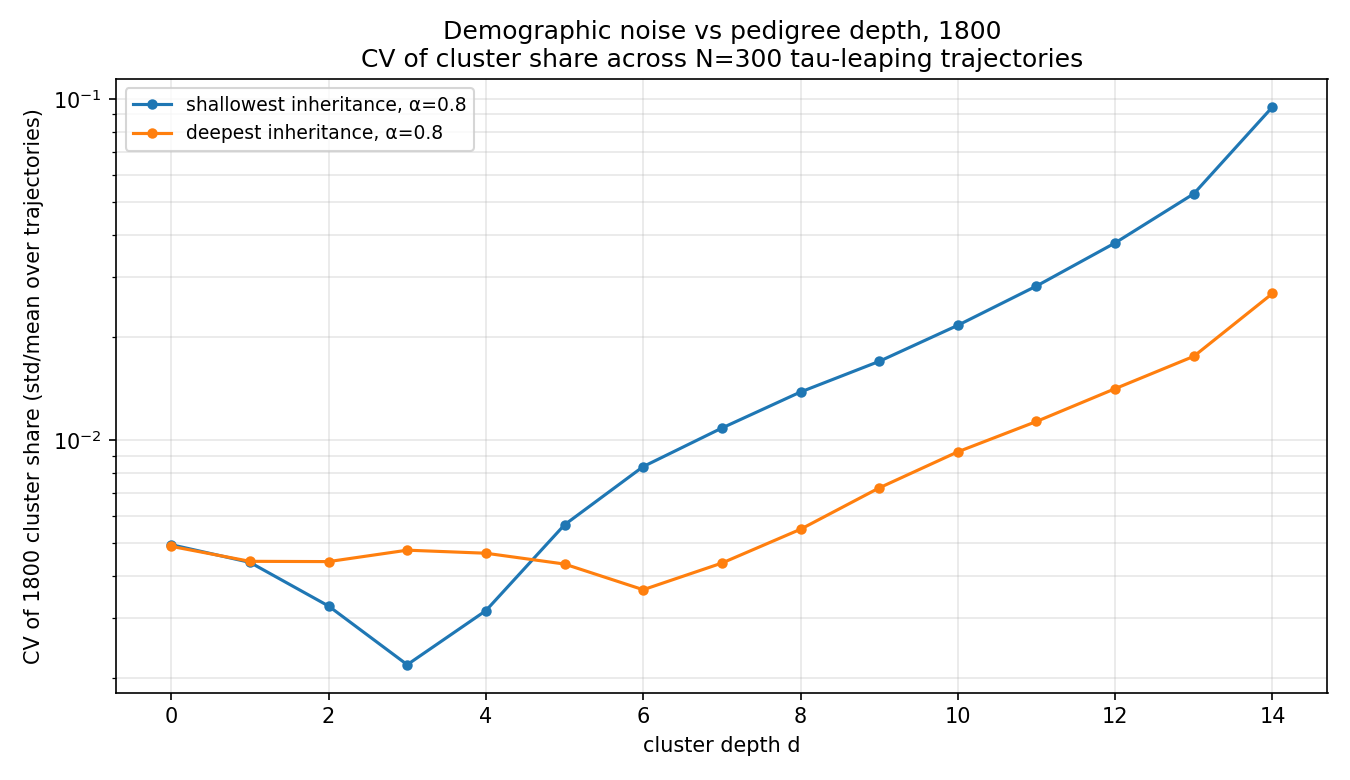
\includegraphics[width=\textwidth]{figs/stochastic_cv_depth.png}
\caption{CV of the 1800 cluster share vs depth $d$, $\alpha=0.8$
(both rules): $C_6$ 0.4--0.8\%, $C_{10}$ 0.9--2.2\%, $C_{14}$
9.5\% (shallowest) / 2.7\% (deepest) --- deep-cluster mass is robust,
not noise-dominated.}
\label{fig:stoch-cv}
\end{figure}

\begin{figure}[htbp]
\centering
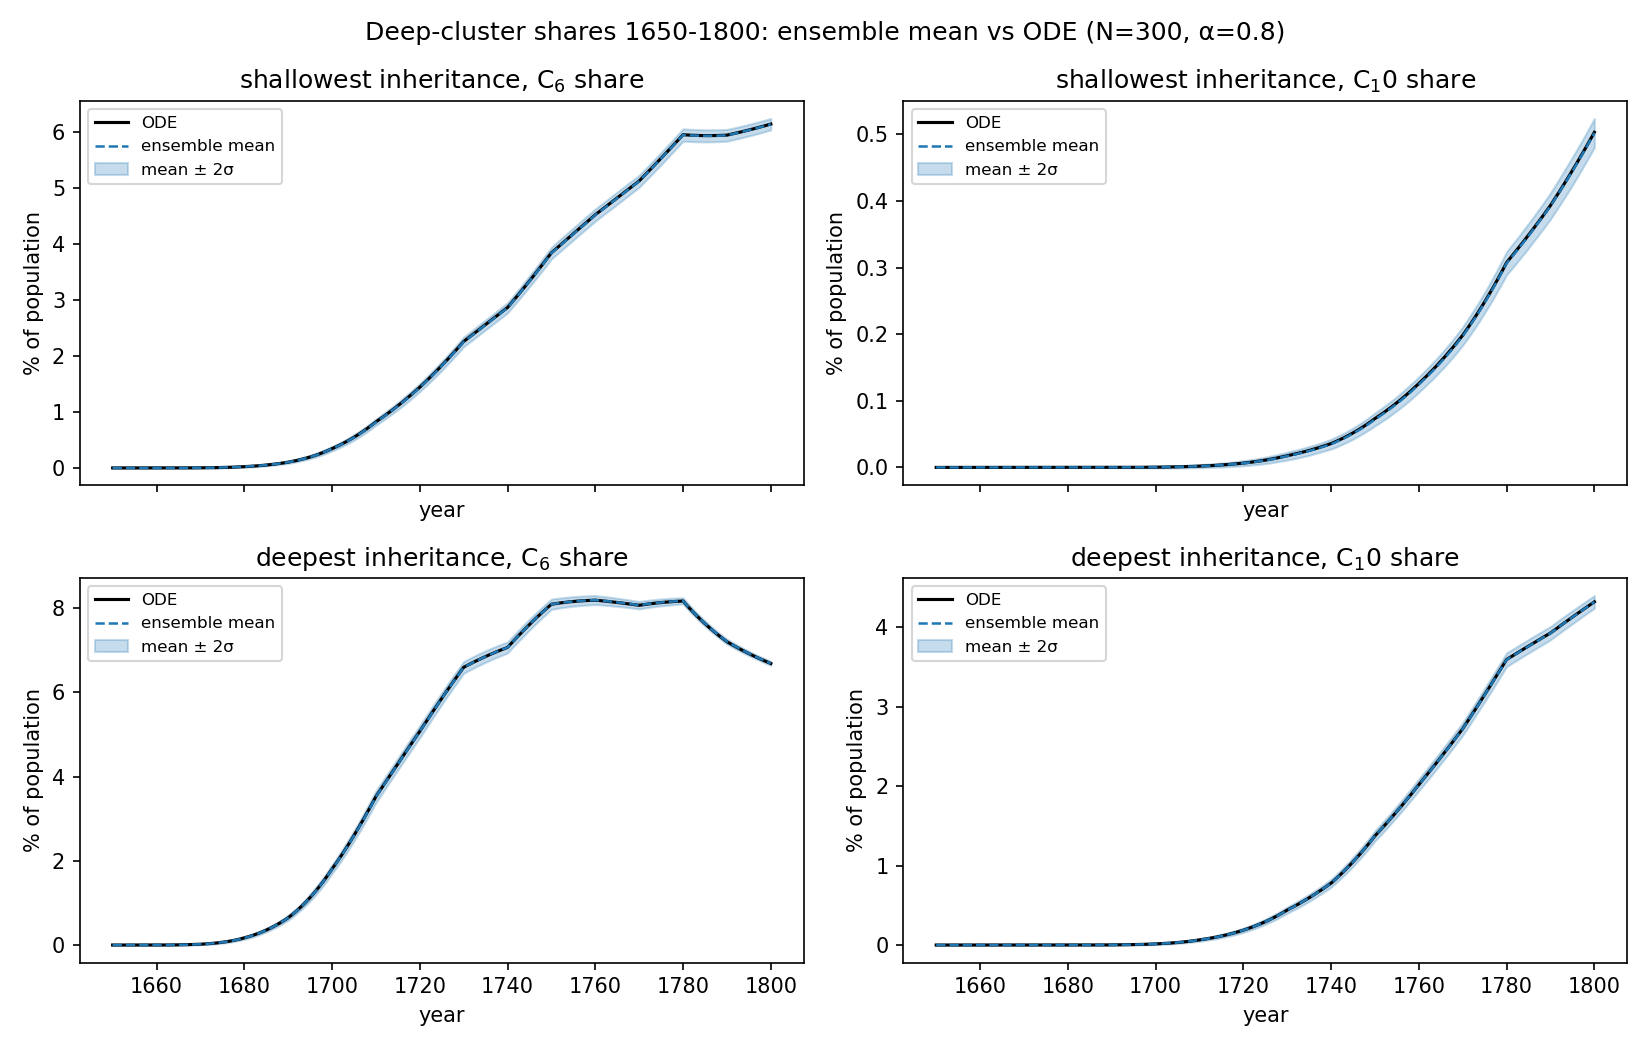
\includegraphics[width=\textwidth]{figs/stochastic_mean_vs_ode.png}
\caption{$C_6$/$C_{10}$ share trajectories 1650--1800, $\alpha=0.8$:
ensemble mean $\pm 2\sigma$ vs ODE (both rules) --- no bias
($|z|\le1.40$, max dev $6.1\times10^{-4}$).}
\label{fig:stoch-mean}
\end{figure}

\begin{figure}[htbp]
\centering
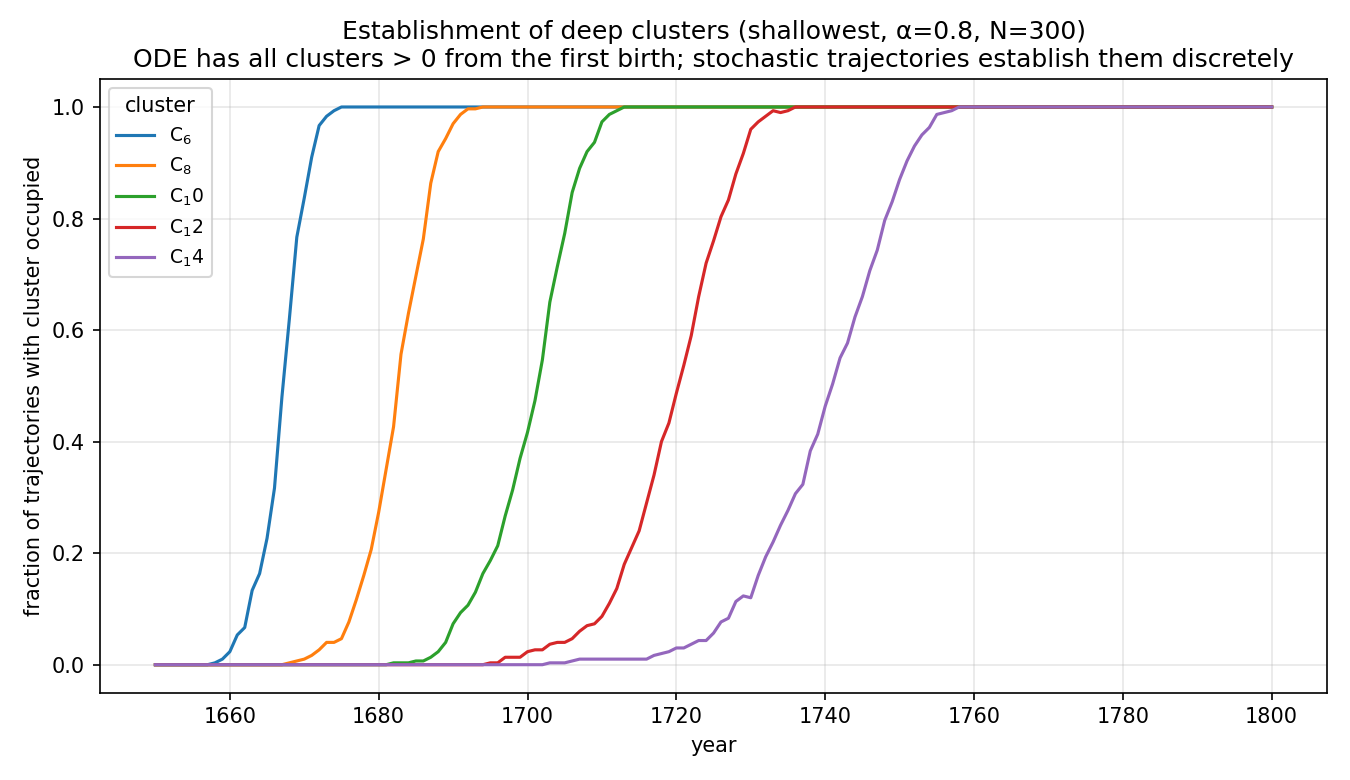
\includegraphics[width=\textwidth]{figs/stochastic_establishment.png}
\caption{Fraction of trajectories with $C_d$ occupied vs year
(shallowest, $\alpha=0.8$): establishment is discrete --- vs the ODE's
``all $>0$ from the first birth''.}
\label{fig:stoch-est}
\end{figure}

\subsection{Independent validation: mixed and informative, not confirmatory}
\label{sec:validation}
Out-of-sample checks of 2025 class shares against Census Bureau data.
All modeled numbers are \emph{predictions} read from the archived
regional colonial run ($\alpha=0.8$, shallowest + deepest); observed data
are \emph{measured} 2023 ACS 1-year survey estimates (table-based
summary files~\cite{acs-2023-b04006-b05002}).  Designs were
pre-specified; no new model runs were made.

\paragraph{(a) Regional ``American''-ancestry check (primary,
pre-specified).}  Observed: \% reporting ``American'' ancestry by
Census region (ACS B04006, measured) --- a documented old-stock proxy,
concentrated in the South.  Modeled: regional 2025 $C_{14}$ share,
$\alpha=0.8$, compared on rank order (Spearman $\rho$) and level.
Result: \textbf{rank flip at the top} --- observed S $>$ MW $>$ NE $>$ W
(7.36 / 4.95 / 4.09 / 3.43\%) vs modeled MW $>$ S $>$ W $>$ NE
(shallowest 0.526 / 0.494 / 0.430 / 0.364\%; deepest 20.61 / 19.54 /
17.20 / 14.74\%; $\rho=0.60$, $n=4$).  The model's ranking is
immigration-dilution arithmetic (the Midwest receives the fewest
immigrants per capita, so deep lineages are least diluted); the
proxy's ranking reflects settlement history and cultural identity the
model does not represent.  This is a \textbf{real structural gap},
stated plainly.  Level: the model underpredicts the proxy under
shallowest (US 0.47\% vs 5.38\%) and overpredicts under deepest (US
18.47\% vs 5.38\%) --- ``American'' self-report is broader than 14
consecutive U.S.-born generations but narrower than the deepest rule's
ratchet; descriptively the proxy's national level lands near modeled
shallowest $C_{10+}$ (3.15\%), i.e.\ $\sim$10+ generations
(post-hoc level match, not a confirmed prediction).

\paragraph{(b) Surname check: a genuine-attempt negative.}  No
defensible operationalization was found with the public 2010 surname
list (151,671 surnames~\cite{census-surnames-2010}).  No check was
performed; documented as a negative result, not an omission.

\paragraph{(c) Foreign-born consistency check.}  Modeled $C_0$ exceeds
observed foreign-born \% by +38\% (W) to +153\% (MW), US +68\%.  The
gap decomposes into documented pieces: the colonial run's 2025 total
(258.9\,M) is 24\% below actual ($\sim$342\,M) while the immigrant
stock is data-driven; model immigration inputs include DHS unauthorized
estimates that ACS undercounts.  Rank order largely holds
($\rho=0.80$).

\begin{figure}[htbp]
\centering
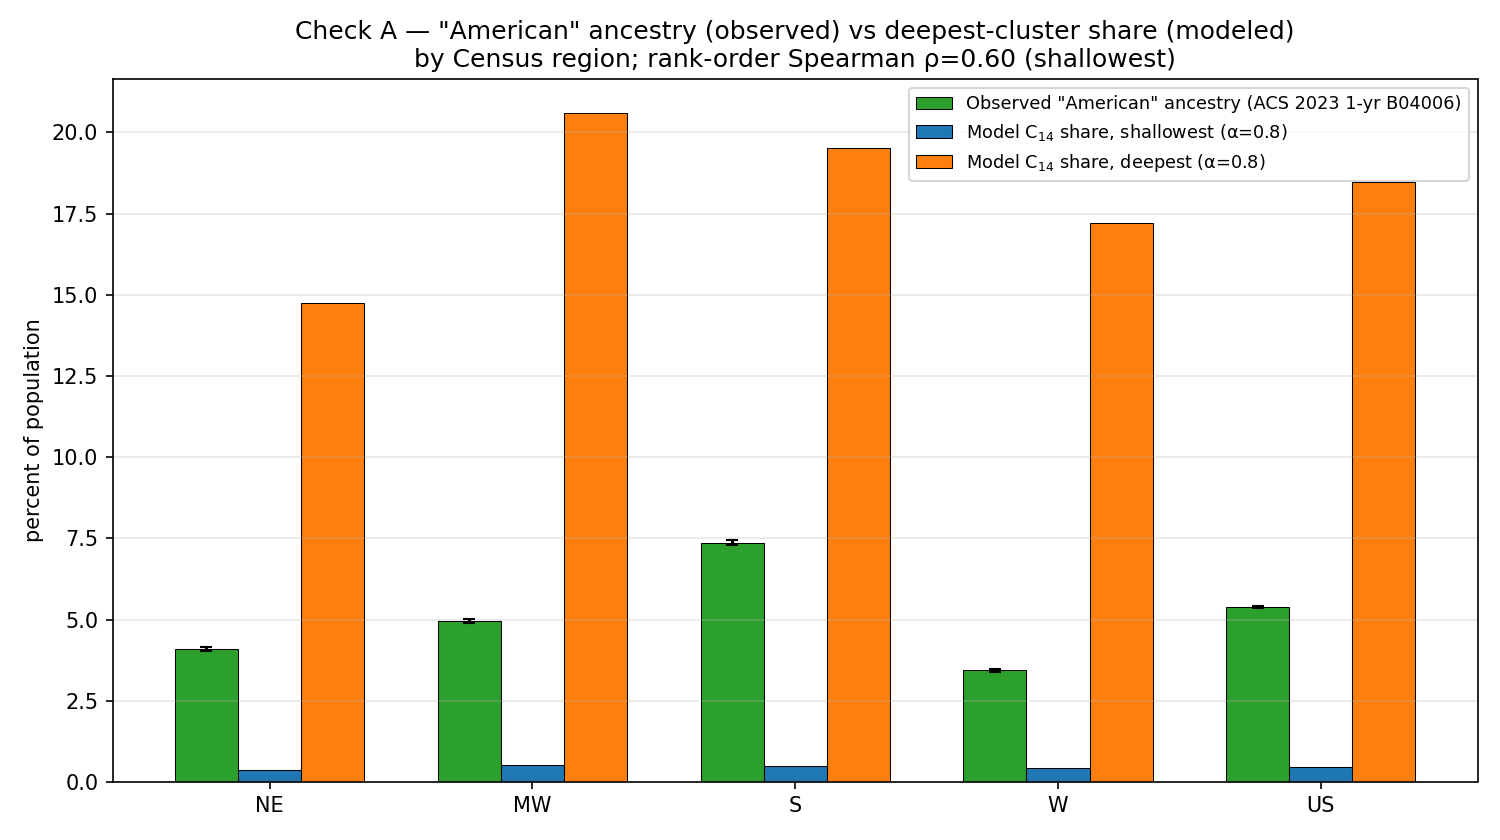
\includegraphics[width=\textwidth]{figs/validation_american_ancestry.png}
\caption{Check (a): observed ``American''-ancestry \% (2023 ACS,
$\pm$MOE) vs modeled 2025 $C_{14}$ \%, by region + US ($\alpha=0.8$).
Rank flip at the top: model peaks MW (immigration-dilution
arithmetic), the proxy peaks S --- a real structural gap
($\rho=0.60$).}
\label{fig:val-ancestry}
\end{figure}

\begin{figure}[htbp]
\centering
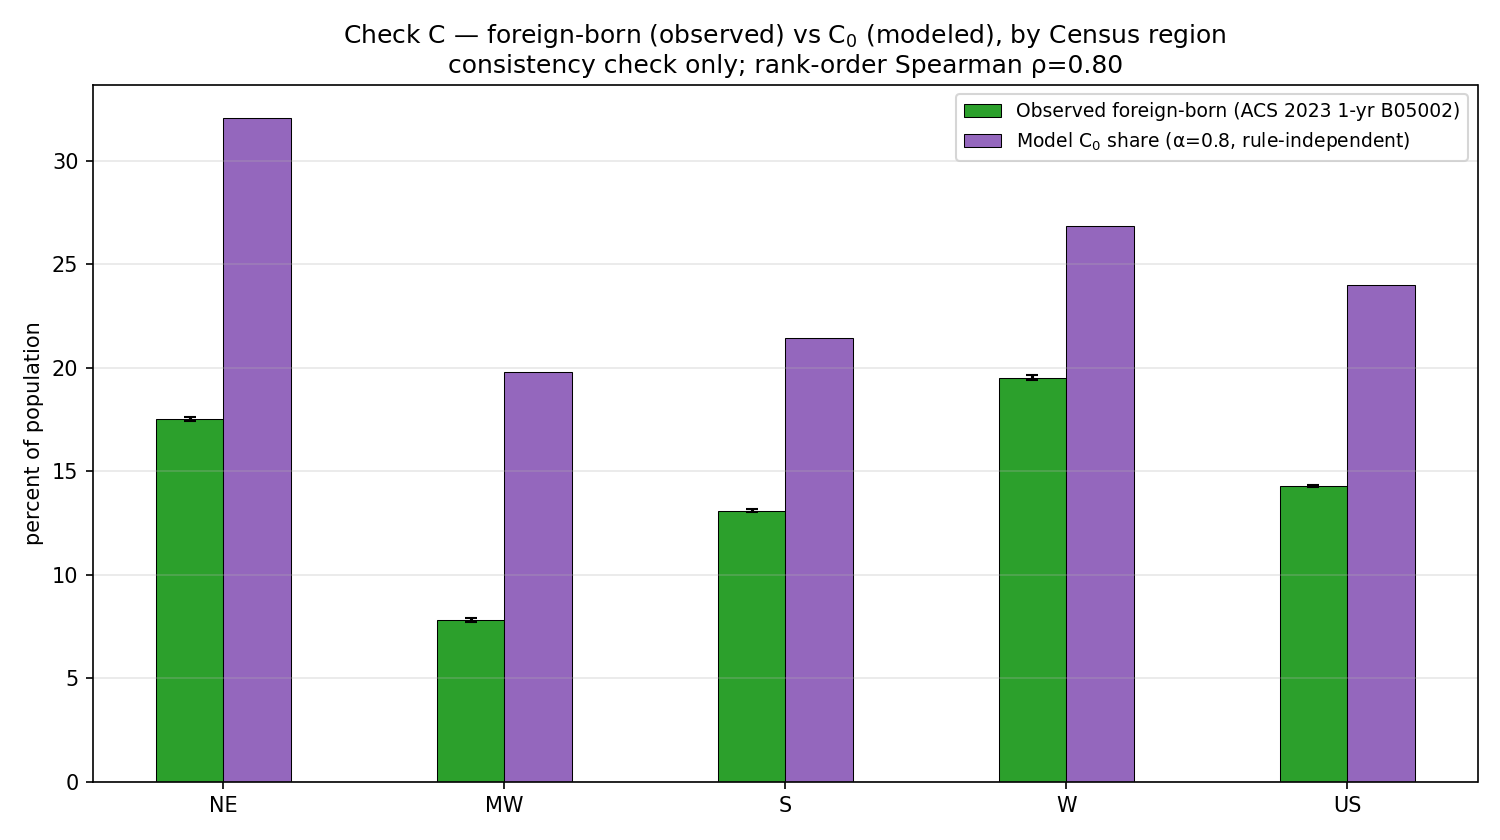
\includegraphics[width=\textwidth]{figs/validation_foreignborn.png}
\caption{Check (c), consistency only: observed foreign-born \%
(2023 ACS) vs modeled 2025 $C_0$ \%, by region + US.  Level
+38--153\% (decomposes into the known total bias +
unauthorized accounting); rank $\rho=0.80$.}
\label{fig:val-foreignborn}
\end{figure}

\section{Suggestions for more accurate models and data}
Completed since the last revision: age structure (Secs.~\ref{sec:age},
\ref{sec:results}), regional compartments (Secs.~\ref{sec:regional},
\ref{sec:results}), the CPS parental-nativity calibration of
$\alpha$ (Sec.~\ref{sec:cps}), time-varying assortativity $\alpha(t)$
(Sec.~6.3, sensitivity variant), sex-specific rates with the
maternal-bottleneck finding (Secs.~2.1, 6.6), deeper cluster resolution
$n=14$ with the tail study (Sec.~6.7), the stochastic colonial era
(Sec.~\ref{sec:stochastic}), and independent validation
(Sec.~\ref{sec:validation}).
\begin{enumerate}
  \item \textbf{Age $\times$ religion interaction.}  The 540-state age
    model and the 240-ODE religious model are verified unbroken but not
    yet combined.
  \item \textbf{Regional vital-rate differences.}  Regional
    fertility/mortality differences and cluster-specific migration are
    unmodeled; regional totals are uncalibrated.
  \item \textbf{Paternal age schedule.}  The male-fertility schedule is
    still the female ASFR shape (\emph{assumed}); a $\sim$2\,yr older
    paternal schedule moves 2025 $C_n$ by 2--5\,pp at $\alpha\ge0.8$
    (Sec.~6.4).  Calibrate from NCHS fatherhood data.
  \item \textbf{$\alpha(t)$ for the extended models.}  The time-varying
    assortativity schedule is implemented only for the two-sex model;
    port it to the religious, age, and regional models.
  \item \textbf{Re-affiliation in disaffiliation.}  The one-way
    disaffiliation flow is an honest artifact (unaffiliated
    27.9\%$\to$36.4\% by 2050); add re-affiliation (two-way religious
    switching).
  \item \textbf{Settlement-history process for regional deep shares.}
    Step 8 found a real structural gap: regional deep-cluster shares
    are set by immigration-dilution arithmetic with no region-specific
    old-stock history or identity process --- the model peaks in the
    Midwest while observed ``American'' ancestry peaks in the South
    (Sec.~\ref{sec:validation}).  Add a settlement-history mechanism
    (or an identity/reporting layer) before the regional deep ranking
    can be trusted.
\end{enumerate}

\vspace{0.3cm}
\begin{center}
\textcolor{nmgray}{\small Code, data pipeline and provenance:
\texttt{genealogy\_dynamics/} --- inputs, calibration, hindcast and
colonial-run scripts with cached public sources.}
\end{center}

% ---------------- 8. References ----------------
\section{References}
\vspace{-1.4em}
\renewcommand{\refname}{}
{\small
\begin{thebibliography}{9}

\bibitem{dhs-yearbook}
U.S.\ Department of Homeland Security, Office of Homeland Security
Statistics. \textit{Yearbook of Immigration Statistics}, Table~1 (LPRs,
1980--2024): measured $I(t)$.

\bibitem{dhs-unauth}
Baker, B.\ and Warren, R., Office of Homeland Security Statistics, U.S.\
Department of Homeland Security. \textit{Estimates of the Unauthorized
Immigrant Population}, various years: augments the legal series for the
hindcast.

\bibitem{wdi}
World Bank. \textit{World Development Indicators}: U.S.\ CBR/CDR,
1960--2024 ($\beta(t)$, $\mu(t)$ from 1960).

\bibitem{nchs-natality}
Martin, J.~A., Hamilton, B.~E., et al. \textit{Births: Final Data for
2024.} NVSR 75(2), NCHS, 2026.  Sex ratio at birth (measured
$s=0.512$).

\bibitem{haines}
Haines, M.~R. ``The Fertility Transition in the United States.''
NBER conference paper, 2002.
\url{https://conference.nber.org/confer/2002/si2002/haines.pdf}
Historical TFR anchors and CDR targets (1800--1949 backcast).

\bibitem{census-hsus}
U.S.\ Bureau of the Census. \textit{Historical Statistics of the United
States, Colonial Times to 1970}, Series Z~1--19 (colonial anchors).

\bibitem{census-decennial}
U.S.\ Census Bureau. \textit{Decennial Census}, 1790--2020 (totals).

\bibitem{inputs-csv}
Ghoniem, N.~M. \texttt{genealogy\_dynamics/data/inputs.csv}: compiled annual
input series, 1650--2024, with per-row \texttt{quality} and
\texttt{quality\_note} flags (this project).

\bibitem{pew-rls-2025}
Pew Research Center. \textit{Religious Landscape Study}, 2023--24:
executive summary and topline.  Feb.\ 2025.  U.S.\ adults: Protestant
40\%, Catholic 19\%, other Christian 3\%, unaffiliated 29\%, Jewish 2\%,
Muslim 1\%, Buddhist 1\%, Hindu 1\%.

\bibitem{pew-intermarriage-2025}
Pew Research Center. ``How Many Married Americans Have Spouses of the Same
Religion.'' Feb.\ 26, 2025.  Same-religion spouses: Mormon 87\%,
Protestant 81\%, Catholic 75\%, unaffiliated 68\%, Jewish 65\%.

\bibitem{pew-jewish-2021}
Pew Research Center. \textit{Jewish Americans in 2020.} May 2021.  58\% of
married Jewish adults have a Jewish spouse (56\% in 2013).

\bibitem{pew-muslim-2017}
Pew Research Center. \textit{U.S.\ Muslims Concerned About Their Place in
Society, but Continue to Believe in the American Dream.} July 2017.  84\%
of married or partnered Muslim Americans have a Muslim spouse/partner.

\bibitem{pew-rls-2008}
Pew Research Center. \textit{U.S.\ Religious Landscape Survey: Religious
Affiliation: Diverse and Dynamic.} Feb.\ 2008.  90\% of married Hindus have
a Hindu spouse.

\bibitem{pew-immig-2013}
Pew Research Center. ``The Religious Affiliation of U.S.\ Immigrants.'' May
2013.  Legal immigrants: Christian 68\% (1992) $\to$ 61\% (2012); Muslim
5\% $\to$ 10\%; Hindu 3\% $\to$ 7\%; Buddhist $\approx$ 7\% $\to$ 6\%;
unaffiliated $\approx$ 14\%.

\bibitem{unwpp-2024}
United Nations, Department of Economic and Social Affairs, Population
Division. \textit{World Population Prospects 2024}, ``Fertility by single
age'' (bulk CSV), USA, Medium variant.
\url{https://population.un.org/wpp/assets/Excel\%20Files/1_Indicator\%20(Standard)/CSV_FILES/WPP2024_Fertility_by_Age1.csv.gz}
ASFR 1950--2023 used for the age-structured $\beta_a(t)$.

\bibitem{hld}
Human Life-Table Database (HLD), USA archive.
\url{https://www.lifetable.de/File/GetDocument/data\%5CUSA\%5CUSA.zip}
$m(x)$, $L(x)$ by single year of age and sex, 1900--2023; used for
$\mu_{s,a}(t)$.

\bibitem{bell-miller}
Bell, F.~C.\ and Miller, M.~L. \textit{Life Tables for the United States
Social Security Area 1900--2100.} SSA Actuarial Study No.~116.
Historical HLD tables 1900--2000.

\bibitem{nchs-lifetables}
National Center for Health Statistics. \textit{United States Life
Tables.} National Vital Statistics Reports, annual and decennial volumes.
HLD tables 2001--2023; also the measured sex ratio at birth $s=0.512$.

\bibitem{acs-migration}
U.S.\ Census Bureau. American Community Survey 1-year State-to-State
Migration Flows, 2023 and 2024.
\url{https://www.census.gov/data/tables/time-series/demo/geographic-mobility/state-to-state-migration.html}
Inter-regional migration rate matrix (measured 2023/2024).

\bibitem{dhs-table4}
U.S.\ Department of Homeland Security, Office of Homeland Security
Statistics. \textit{Yearbook of Immigration Statistics 2023}, Table~4:
Persons Obtaining Lawful Permanent Resident Status by State or Territory
of Residence, FY2014--2023.
\url{https://ohss.dhs.gov/topics/immigration/yearbook/2023/table4}
Regional immigration allocation shares (measured 2014--2023).

\bibitem{cps-asec-2024}
U.S.\ Census Bureau. Current Population Survey, 2024 Annual Social and
Economic Supplement, ``Foreign-Born: 2024 Current Population Survey
Detailed Tables,'' Table~1: Population by Generation, 2005--2024.
Released September 2025.
\url{https://www.census.gov/data/tables/2024/demo/foreign-born/cps-2024.html}
Annual second-generation shares (measured).

\bibitem{p23-214}
Trevelyan, E.~N., et al. \textit{Characteristics of the U.S.\ Population
by Generational Status: 2013.} U.S.\ Census Bureau, Current Population
Reports, P23-214, 2016.
\url{https://www.census.gov/content/dam/Census/library/publications/2016/demo/P23-214.pdf}
2013 generation shares and the 59\% two-foreign-born-parent split among
the second generation (measured); the $\alpha$ calibration anchor.

\bibitem{pew-secondgen-2013}
Pew Research Center. ``Second-Generation Americans: A Portrait of the
Adult Children of Immigrants.'' February 2013.
Contextual second-generation levels (36M in 2012; 10\% in 1990).

\bibitem{pew-intermarriage-2023}
Pew Research Center. ``Interracial Marriage Grows.'' June 15, 2023.
Newlywed intermarriage share used for the measured $\alpha(t)$
1959--2015 segment.

\bibitem{livingston-brown-2017}
Livingston, G.\ and Brown, A., Pew Research Center. ``Intermarriage in
the U.S.\ 50 Years After \textit{Loving v.\ Virginia}.'' May 18, 2017.

\bibitem{pew-interfaith-2015}
Pew Research Center. ``Interfaith marriage is common in U.S.,
particularly among the recently wed.'' June 2, 2015. Corroboration for
the post-1960 decline segment of $\alpha(t)$.

\bibitem{pagnini-morgan-1990}
Pagnini, D.\ L.\ and Morgan, S.\ P.\ ``Intermarriage and Social Distance
Among U.S.\ Immigrants at the Turn of the Century.'' \textit{American
Journal of Sociology} 96 (2), 1990. Used for the 1910 $\alpha(t)$
anchor.

\bibitem{draschler-1921}
Draschler, J.\ \textit{Intermarriage in New York City: A Statistical
Study of the Amalgamation of European Peoples}. Columbia University
Press, 1921. NYC license data 1908--12 used for the 1910
$\alpha(t)$ anchor.

\bibitem{logan-shin-2012}
Logan, J.\ R.\ and Shin, H.-b.\ ``Assimilation by the Third
Generation?'' \textit{International Migration Review} 46 (3), 2012.
Used for the 1880 $\alpha(t)$ anchor.

\bibitem{alba-golden-1986}
Alba, R.\ D.\ and Golden, R.\ M.\ ``Patterns of Ethnic Marriage in the
United States.'' \textit{Social Forces} 65 (1), 1986. Used for the 1850
$\alpha(t)$ anchor.

\bibitem{alba-1983}
Alba, R.\ D.\ \textit{Italian Americans: Into the Twilight of
Ethnicity}. Prentice-Hall, 1983. Used for the 1940 $\alpha(t)$ anchor.

\bibitem{spoerlein-2014}
Sp\"orlein, C.\ et~al.\ ``Assortative mating and the intergenerational
transmission of socioeconomic status.'' 2014. Used for the 1880
$\alpha(t)$ anchor.

\bibitem{hsus-immig}
Haines, M.\ R.\ et~al., \textit{Historical Statistics of the United
States}, Millennial Edition: Table~Aa essay (62.9\% male among
immigrants 1820--1917, estimated $\sigma=0.629$ for that span) and
Table~Ad immigration essay (convergence toward parity by 1950).

\bibitem{dhs-lpr-sex}
U.S.\ Department of Homeland Security, Office of Homeland Security
Statistics. \textit{Yearbook of Immigration Statistics}, Table~9 (LPR
admissions by sex, 2015--2023): measured component of $\sigma(t)$.

\bibitem{dhs-unauth-table4}
U.S.\ Department of Homeland Security, Office of Homeland Security
Statistics. Unauthorized-immigrant population estimates, Table~4
(sex composition of the unauthorized stock): proxy for the sex
composition of unauthorized inflow, estimated component of
$\sigma(t)$.

\bibitem{gillespie-1976}
Gillespie, D.~T. ``A general method for numerically simulating the
stochastic time evolution of coupled chemical reactions.''
\textit{J.\ Comput.\ Phys.} 22(4), 403--434, 1976.  Exact SSA: the
jump process simulated in Sec.~\ref{sec:stochastic}.

\bibitem{gillespie-2001}
Gillespie, D.~T. ``Approximate accelerated stochastic simulation of
chemically reacting systems.'' \textit{J.\ Chem.\ Phys.} 115(4),
1716--1733, 2001.  $\tau$-leaping (Sec.~\ref{sec:stochastic}).

\bibitem{cao-gillespie-petzold-2006}
Cao, Y., Gillespie, D.~T.\ and Petzold, L.~R. ``Efficient step size
selection for the tau-leaping simulation method.'' \textit{J.\ Chem.\
Phys.} 124(4), 044109, 2006.  Adaptive $\tau$ selection.

\bibitem{kurtz-1970}
Kurtz, T.~G. ``Solutions of ordinary differential equations as limits
of pure jump Markov processes.'' \textit{J.\ Appl.\ Probab.} 7(1),
49--58, 1970.  Mean-field/density-dependent limit: scaled jump process
$\to$ ODE.

\bibitem{acs-2023-b04006-b05002}
U.S.\ Census Bureau. 2023 American Community Survey 1-year estimates,
Detailed Table B04006 (People Reporting Ancestry) and Table B05002
(Place of Birth by Nativity and Citizenship Status), table-based
summary files, accessed 2026-09-26.
\url{https://www2.census.gov/programs-surveys/acs/summary_file/2023/table-based-SF/data/1YRData/}
Variable metadata via
\url{https://api.census.gov/data/2023/acs/acs1/variables.json}.
Observed data for the independent validation (Sec.~\ref{sec:validation}).

\bibitem{census-surnames-2010}
U.S.\ Census Bureau. Frequently Occurring Surnames from the 2010
Census, file \texttt{Names\_2010Census.csv}, accessed 2026-09-26.
\url{https://www2.census.gov/topics/genealogy/2010surnames/names.zip}
Downloaded and inspected; no defensible check found
(Sec.~\ref{sec:validation}).

\bibitem{chang1999}
Chang, J.~T. Recent common ancestors of all present-day individuals.
\textit{Adv.\ Appl.\ Probab.} 31, 1002--1026 (1999).

\bibitem{rohde2004}
Rohde, D.~L.~T., Olson, S.\ and Chang, J.~T. Modelling the recent common
ancestry of all living humans. \textit{Nature} 431, 562--566 (2004).

\bibitem{derrida1999}
Derrida, B., Manrubia, S.~C.\ and Zanette, D.~H. Statistical properties of
genealogical trees. \textit{Phys.\ Rev.\ Lett.} 82, 1987--1990 (1999).

\bibitem{derrida2000}
Derrida, B., Manrubia, S.~C.\ and Zanette, D.~H. On the genealogy of a
population of biparental individuals. \textit{J.\ Theor.\ Biol.} 203,
303--315 (2000).

\bibitem{manrubia2002}
Manrubia, S.~C.\ and Zanette, D.~H. At the boundary between biological and
cultural evolution: the origin of surname distributions. \textit{J.\
Theor.\ Biol.} 216, 461--477 (2002).

\bibitem{cavalli-sforza1981}
Cavalli-Sforza, L.~L.\ and Feldman, M.~W. \textit{Cultural Transmission and
Evolution: A Quantitative Approach.} Princeton University Press (1981).

\bibitem{matsen2008}
Matsen, F.~A.\ and Evans, S.~N. To what extent does genealogical ancestry
imply genetic ancestry? \textit{Theor.\ Popul.\ Biol.} 74, 182--190 (2008).

\end{thebibliography}
}

\end{document}
